% Options for packages loaded elsewhere
\PassOptionsToPackage{unicode}{hyperref}
\PassOptionsToPackage{hyphens}{url}
%
\documentclass[
]{article}
\usepackage{amsmath,amssymb}
\usepackage{lmodern}
\usepackage{iftex}
\ifPDFTeX
  \usepackage[T1]{fontenc}
  \usepackage[utf8]{inputenc}
  \usepackage{textcomp} % provide euro and other symbols
\else % if luatex or xetex
  \usepackage{unicode-math}
  \defaultfontfeatures{Scale=MatchLowercase}
  \defaultfontfeatures[\rmfamily]{Ligatures=TeX,Scale=1}
\fi
% Use upquote if available, for straight quotes in verbatim environments
\IfFileExists{upquote.sty}{\usepackage{upquote}}{}
\IfFileExists{microtype.sty}{% use microtype if available
  \usepackage[]{microtype}
  \UseMicrotypeSet[protrusion]{basicmath} % disable protrusion for tt fonts
}{}
\makeatletter
\@ifundefined{KOMAClassName}{% if non-KOMA class
  \IfFileExists{parskip.sty}{%
    \usepackage{parskip}
  }{% else
    \setlength{\parindent}{0pt}
    \setlength{\parskip}{6pt plus 2pt minus 1pt}}
}{% if KOMA class
  \KOMAoptions{parskip=half}}
\makeatother
\usepackage{xcolor}
\usepackage[margin=1in]{geometry}
\usepackage{graphicx}
\makeatletter
\def\maxwidth{\ifdim\Gin@nat@width>\linewidth\linewidth\else\Gin@nat@width\fi}
\def\maxheight{\ifdim\Gin@nat@height>\textheight\textheight\else\Gin@nat@height\fi}
\makeatother
% Scale images if necessary, so that they will not overflow the page
% margins by default, and it is still possible to overwrite the defaults
% using explicit options in \includegraphics[width, height, ...]{}
\setkeys{Gin}{width=\maxwidth,height=\maxheight,keepaspectratio}
% Set default figure placement to htbp
\makeatletter
\def\fps@figure{htbp}
\makeatother
\setlength{\emergencystretch}{3em} % prevent overfull lines
\providecommand{\tightlist}{%
  \setlength{\itemsep}{0pt}\setlength{\parskip}{0pt}}
\setcounter{secnumdepth}{5}
\newlength{\cslhangindent}
\setlength{\cslhangindent}{1.5em}
\newlength{\csllabelwidth}
\setlength{\csllabelwidth}{3em}
\newlength{\cslentryspacingunit} % times entry-spacing
\setlength{\cslentryspacingunit}{\parskip}
\newenvironment{CSLReferences}[2] % #1 hanging-ident, #2 entry spacing
 {% don't indent paragraphs
  \setlength{\parindent}{0pt}
  % turn on hanging indent if param 1 is 1
  \ifodd #1
  \let\oldpar\par
  \def\par{\hangindent=\cslhangindent\oldpar}
  \fi
  % set entry spacing
  \setlength{\parskip}{#2\cslentryspacingunit}
 }%
 {}
\usepackage{calc}
\newcommand{\CSLBlock}[1]{#1\hfill\break}
\newcommand{\CSLLeftMargin}[1]{\parbox[t]{\csllabelwidth}{#1}}
\newcommand{\CSLRightInline}[1]{\parbox[t]{\linewidth - \csllabelwidth}{#1}\break}
\newcommand{\CSLIndent}[1]{\hspace{\cslhangindent}#1}
\usepackage{setspace}\doublespacing
\usepackage[fontsize=12pt]{scrextend}
\usepackage[left]{lineno}
\usepackage[labelformat=empty]{caption}
\usepackage{longtable}
\usepackage{booktabs}
\usepackage{booktabs}
\usepackage{longtable}
\usepackage{array}
\usepackage{multirow}
\usepackage{wrapfig}
\usepackage{float}
\usepackage{colortbl}
\usepackage{pdflscape}
\usepackage{tabu}
\usepackage{threeparttable}
\usepackage{threeparttablex}
\usepackage[normalem]{ulem}
\usepackage{makecell}
\usepackage{xcolor}
\ifLuaTeX
  \usepackage{selnolig}  % disable illegal ligatures
\fi
\IfFileExists{bookmark.sty}{\usepackage{bookmark}}{\usepackage{hyperref}}
\IfFileExists{xurl.sty}{\usepackage{xurl}}{} % add URL line breaks if available
\urlstyle{same} % disable monospaced font for URLs
\hypersetup{
  hidelinks,
  pdfcreator={LaTeX via pandoc}}

\author{}
\date{\vspace{-2.5em}}

\begin{document}

\hypertarget{title-page}{%
\section{Title Page}\label{title-page}}

\textbf{Bimodal inference in humans and mice}\\
\strut \\

\textbf{Authors}:

Veith Weilnhammer\(^{1,2}\), Heiner Stuke\(^{1,2}\), Kai
Standvoss\(^{1,3,5}\), Philipp Sterzer\(^{1,3,4,5}\)\\
\strut \\
\textbf{Affiliations}:

\(^{1}\) Department of Psychiatry, Charité-Universitätsmedizin Berlin,
corporate member of Freie Universität Berlin and Humboldt-Universität zu
Berlin, 10117 Berlin, Germany\\
\(^{2}\) Berlin Institute of Health, Charité-Universitätsmedizin Berlin
and Max Delbrück Center, 10178 Berlin, Germany\\
\(^{3}\) Bernstein Center for Computational Neuroscience,
Charité-Universitätsmedizin Berlin, 10117 Berlin, Germany\\
\(^{4}\) Berlin School of Mind and Brain, Humboldt-Universität zu
Berlin, 10099 Berlin, Germany\\
\(^{5}\) Einstein Center for Neurosciences Berlin, 10117 Berlin,
Germany\\
\strut \\

\textbf{Corresponding Author}:

Veith Weilnhammer, Department of Psychiatry, Charité Campus Mitte,
Charitéplatz 1, 10117 Berlin, phone: 0049 (0)30 450 517 317, email:
\href{mailto:veith.weilnhammer@gmail.com}{\nolinkurl{veith.weilnhammer@gmail.com}}\\

\newpage

\linenumbers

\hypertarget{abstract}{%
\section{Abstract}\label{abstract}}

Perception is known to cycle through periods of enhanced and reduced
sensitivity to external information. Here, we asked whether such
infra-slow fluctuations arise as a noise-related epiphenomenon of
limited processing capacity or, alternatively, represent a structured
mechanism of perceptual inference. Using two large-scale datasets, we
found that humans and mice waver between alternating intervals of
externally- and internally-oriented modes of sensory analysis. During
external mode, perception aligned more closely with the external sensory
information, whereas internal mode was characterized by enhanced biases
toward perceptual history. Computational modeling indicated that dynamic
changes in mode are enabled by two interlinked factors: (i), the
integration of subsequent inputs over time and, (ii), infra-slow
anti-phase oscillations in the perceptual impact of external sensory
information versus internal predictions that are provided by perceptual
history. Simulated data suggested that between-mode fluctuations may
benefit perception by generating unambiguous error signals that enable
robust learning and metacognition in volatile environments.

\hypertarget{one-sentence-summary}{%
\section{One sentence summary}\label{one-sentence-summary}}

Humans and mice fluctuate between external and internal modes of sensory
processing.

\hfill\break

\newpage

\hypertarget{introduction}{%
\section{Introduction}\label{introduction}}

The capacity to respond to changes in the environment is a defining
feature of life\textsuperscript{1--3}. Intriguingly, the ability of
living things to process their surroundings fluctuates considerably over
time\textsuperscript{4,5}. In humans and mice,
perception\textsuperscript{6--12}, cognition\textsuperscript{13} and
memory\textsuperscript{14} cycle through prolonged periods of enhanced
and reduced sensitivity to external information, suggesting that the
brain detaches from the world in recurring intervals that last from
milliseconds to seconds and even minutes\textsuperscript{4,5}. Yet
breaking from external information is risky, as swift responses to the
environment are often crucial to survival.

What could be the reason for these fluctuations in perceptual
performance\textsuperscript{11}? First, periodic fluctuations in the
ability to parse external information\textsuperscript{11,15,16} may
arise simply due to bandwidth limitations and noise. Second, it may be
advantageous to actively reduce the costs of neural processing by
seeking sensory information only in recurring
intervals\textsuperscript{5,17}, otherwise relying on random or
stereotypical responses to the external world. Third, spending time away
from the ongoing stream of sensory inputs may also reflect a functional
strategy that facilitates flexible behavior and
learning\textsuperscript{18}: Intermittently relying more strongly on
information acquired from past experiences may enable agents to build up
stable internal predictions about the environment despite an ongoing
stream of external sensory signals\textsuperscript{19}. By the same
token, recurring intervals of enhanced sensitivity to external
information may help to detect changes in both the state of the
environment and the amount of noise that is inherent in sensory
encoding\textsuperscript{19}.

In this work, we sought to elucidate whether periodicities in the
sensitivity to external information represent an epiphenomenon of
limited processing capacity or, alternatively, result from a structured
and adaptive mechanism of perceptual inference. To this end, we analyzed
two large-scale datasets on perceptual decision-making in
humans\textsuperscript{20} and mice\textsuperscript{21}. When less
sensitive to external stimulus information, humans and mice showed
stronger serial dependencies\textsuperscript{22--33}, which have been
conceptualized as internal predictions that reflect the auto-correlation
of natural environments\textsuperscript{34} and bias perceptual
decisions toward preceding choices\textsuperscript{30,31,35}.
Computational modeling indicated that ongoing changes in perceptual
performance may be driven by systematic fluctuations between externally-
and internally-oriented modes of sensory analysis. Model simulations
suggested that such bimodal inference may improve, (i), the ability to
robustly determine the statistical properties of volatile environments
and, (ii), the ability to calibrate internal beliefs about the degree of
noise inherent in the encoding of sensory information.

\hypertarget{results}{%
\section{Results}\label{results}}

\hypertarget{human-perception-fluctuates-between-epochs-of-enhanced-and-reduced-sensitivity-to-external-information}{%
\subsection{Human perception fluctuates between epochs of enhanced and
reduced sensitivity to external
information}\label{human-perception-fluctuates-between-epochs-of-enhanced-and-reduced-sensitivity-to-external-information}}

We began by selecting 66 studies from the Confidence
Database\textsuperscript{20} that investigated how human participants (N
= 4317) perform binary perceptual decisions (Figure 1A; see Methods
section for details on inclusion criteria). As a metric for perceptual
performance (i.e., the sensitivity to external sensory information), we
asked whether the participant's response and the presented stimulus
matched (\emph{stimulus-congruent} choices) or differed from each other
(\emph{stimulus-incongruent} choices; Figure 1B and C) in a total of
\(21.05\) million trials.

In a first step, we asked whether the ability to accurately perceive
sensory stimuli is constant over time or, alternatively, fluctuates in
periods of enhanced and reduced sensitivity to external information. We
found perception to be stimulus-congruent in 73.46\% ± 0.15\% of trials
(mean ± standard error of the mean; Figure 2A), which was highly
consistent across the selected studies (Supplemental Figure S1A). In
line with previous work\textsuperscript{8}, we found that the
probability of stimulus-congruence was not independent across successive
trials: At the group level, stimulus-congruent perceptual choices were
significantly autocorrelated for up to 15 trials. Autocorrelation
coefficients decayed exponentially over time (rate \(\gamma\) =
\(\ensuremath{-1.92\times 10^{-3}}\) ±
\(\ensuremath{4.5\times 10^{-4}}\),
T(\(\ensuremath{6.88\times 10^{4}}\)) = \(-4.27\), p =
\(\ensuremath{1.98\times 10^{-5}}\); Figure 2B). Importantly, the
autocorrelation of stimulus-congruent perception was not a trivial
consequence of the experimental design, but remained significant when
controlling for the trial-wise autocorrelation of task difficulty
(Supplemental Figure S2A) or the sequence of presented stimuli
(Supplemental Figure S2B).

In addition, stimulus-congruence was significantly autocorrelated not
only at the group-level, but also in individual participants, where the
autocorrelation of stimulus-congruent perception exceeded the respective
autocorrelation of randomly permuted data within an interval of 3.24 ±
\ensuremath{2.39\times 10^{-3}} trials (Figure 2C). In other words, if a
participant's experience was congruent (or incongruent) with the
external stimulus information at a given trial, her perception was more
likely to be stimulus-congruent (or incongruent) for approximately 3
trials into the future.

To further corroborate the autocorrelation of stimulus-congruence, we
used logistic regression models that predicted the stimulus-congruence
of perception at the index trial \(t = 0\) from the stimulus-congruence
at the preceding trials within a lag of 25 trials. We found that
regression weights were significantly greater than zero for up to 16
trials (Supplemental Figure S3).

These results confirm that the ability to process sensory signals is not
constant over time, but unfolds in multi-trial epochs of enhanced and
reduced sensitivity to external information\textsuperscript{8}. As a
consequence of this autocorrelation, the dynamic probability of
stimulus-congruent perception (i.e., computed in sliding windows of ± 5
trials; Figure 1C) fluctuated considerably within participants (average
minimum: 35.46\% ± 0.22\%, maximum: 98.27\% ± 0.07\%). In line with
previous findings\textsuperscript{9}, such fluctuations in the
sensitivity to external information had a power density that was
inversely proportional to the frequency in the infra-slow
spectrum\textsuperscript{11} (power \textasciitilde{} 1/\(f^\beta\),
\(\beta\) = \(-1.32\) ± \(\ensuremath{3.14\times 10^{-3}}\),
T(\(\ensuremath{1.84\times 10^{5}}\)) = \(-419.48\), p < \(\ensuremath{2.2\times 10^{-308}}\); Figure
2D). This feature, which is also known as \emph{1/f
noise}\textsuperscript{36,37}, represents a characteristic of ongoing
fluctuations in complex dynamic systems such as the
brain\textsuperscript{38} and the cognitive processes it
entertains\textsuperscript{9,10,13,39,40}.

\hypertarget{human-perception-fluctuates-between-external-and-internal-modes-of-sensory-processing}{%
\subsection{Human perception fluctuates between external and internal
modes of sensory
processing}\label{human-perception-fluctuates-between-external-and-internal-modes-of-sensory-processing}}

In a second step, we sought to explain why perception cycles through
periods of enhanced and reduced sensitivity to external
information\textsuperscript{4,5}. We reasoned that observers may
intermittently rely more strongly on internal information, i.e., on
predictions about the environment that are constructed from previous
experiences\textsuperscript{19,31}.

In perception, \emph{serial dependencies} represent one of the most
basic internal predictions that cause perceptual decisions to be
systematically biased toward preceding choices\textsuperscript{22--33}.
Such effects of perceptual history mirror the continuity of the external
world, in which the recent past often predicts the near
future\textsuperscript{30,31,34,35,41}. Therefore, as a metric for the
perceptual impact of internal information, we computed whether the
participant's response at a given trial matched or differed from her
response at the preceding trial (\emph{history-congruent} and
\emph{history-incongruent perception}, respectively; Figure 1B and C).

First, we ensured that perceptual history played a significant role in
perception despite the ongoing stream of external information. With a
global average of 52.7\% ± 0.12\% history-congruent trials, we found a
small but highly significant perceptual bias towards preceding
experiences (\(\beta\) = \(16.18\) ± \(1.07\),
T(\(\ensuremath{1.09\times 10^{3}}\)) = \(15.07\), p =
\(\ensuremath{10^{-46}}\); Figure 2A) that was largely consistent across
studies (Supplemental Figure 1B) and more pronounced in participants who
were less sensitive to external sensory information (Supplemental Figure
1C). Logistic regression confirmed the internal information provided by
perceptual history made a significant contribution to perception
(\(\beta\) = \(0.11\) ± \(\ensuremath{5.79\times 10^{-3}}\), z =
\(18.53\), p = \(\ensuremath{1.1\times 10^{-76}}\)) over and above the
ongoing stream of external sensory information (\(\beta\) = \(2.2\) ±
\(\ensuremath{5.87\times 10^{-3}}\), z = \(375.11\), p < \(\ensuremath{2.2\times 10^{-308}}\)) and
general response biases toward one of the two potential outcomes
(\(\beta\) = \(15.19\) ± \(0.08\), z = \(184.98\), p < \(\ensuremath{2.2\times 10^{-308}}\); see
Supplemental Figure S4A for model comparisons within individual
participants).

In addition, we confirmed that history-congruence was not a corollary of
the sequence of presented stimuli: History-congruent perceptual choices
were more frequent at trials when perception was stimulus-incongruent
(56.03\% ± 0.2\%) as opposed to stimulus-congruent (51.77\% ± 0.11\%,
\(\beta\) = \(-4.26\) ± \(0.21\), T(\(\ensuremath{8.57\times 10^{3}}\))
= \(-20.36\), p = \(\ensuremath{5.28\times 10^{-90}}\); Figure 2A, lower
panel). Despite being adaptive in auto-correlated real-world
environments\textsuperscript{19,34,35,42}, perceptual history thus
represented a source of error in the randomized experimental designs
studied here\textsuperscript{24,28,30,31,43}.

Second, we asked whether perception cycles through multi-trial epochs
during which perception is characterized by stronger or weaker biases
toward preceding experiences. Indeed, in close analogy to
stimulus-congruence, history-congruence was significantly autocorrelated
for up to 21 trials (Figure 2B). Following a peak at the first trial,
the respective autocorrelation coefficients decreased exponentially over
time (rate \(\gamma\) = \(\ensuremath{-6.11\times 10^{-3}}\) ±
\(\ensuremath{5.69\times 10^{-4}}\),
T(\(\ensuremath{6.75\times 10^{4}}\)) = \(-10.74\), p =
\(\ensuremath{7.18\times 10^{-27}}\)). History-congruence remained
significantly autocorrelated when controlling for task difficulty
(Supplemental Figure S2A) and the sequence of presented stimuli
(Supplemental Figure S2B). In individual participants, the
autocorrelation of history-congruence was elevated above randomly
permuted data for a lag of 4.87 ± \ensuremath{3.36\times 10^{-3}} trials
(Figure 2C), confirming that the autocorrelation of history-congruence
was not only a group-level phenomenon. The autocorrelation of
history-congruence was confirmed by logistic regression models that
successfully predicted the history-congruence of perception at an index
trial \(t = 0\) from the history-congruence at the preceding trials
within a lag of 17 trials (Supplemental Figure S3).

Third, we asked whether the impact of internal information fluctuates as
1/f noise (i.e., a noise characteristic classically associated with
fluctuations in the sensitivity to external
information\textsuperscript{9,10,13,39,40}). The dynamic probability of
history-congruent perception (i.e., computed in sliding windows of ± 5
trials; Figure 1C) varied considerably over time, ranging between a
minimum of 12.77\% ± 0.14\% and a maximum 92.23\% ± 0.14\%. In analogy
to stimulus-congruence, we found that history-congruence fluctuated as
1/f noise, with power densities that were inversely proportional to the
frequency in the infra-slow spectrum\textsuperscript{11} (power
\textasciitilde{} 1/\(f^\beta\), \(\beta\) = \(-1.34\) ±
\(\ensuremath{3.16\times 10^{-3}}\),
T(\(\ensuremath{1.84\times 10^{5}}\)) = \(-423.91\), p < \(\ensuremath{2.2\times 10^{-308}}\); Figure
2D).

Finally, we ensured that fluctuations in stimulus- and
history-congruence are linked to each other. When perceptual choices
were less biased toward external information, participants relied more
strongly on internal information acquired from perceptual history (and
vice versa, \(\beta\) = \(-0.1\) ± \(\ensuremath{8.59\times 10^{-4}}\),
T(\(\ensuremath{2.1\times 10^{6}}\)) = \(-110.96\), p < \(\ensuremath{2.2\times 10^{-308}}\)). Thus,
while sharing the characteristic of 1/f noise, fluctuations in stimulus-
and history-congruence were shifted against each other by approximately
half a cycle and showed a squared coherence of 6.49 ±
\ensuremath{2.07\times 10^{-3}}\% (Figure 2E and F; we report the
average phase and coherence for frequencies below 0.1 \(1/N_{trials}\);
see Methods for details).

In sum, our analyses indicate that perceptual decisions may result from
a competition between external sensory signals with internal predictions
provided by perceptual history. Crucially, we show that the impact of
these external and internal sources of information is not stable over
time, but fluctuates systematically, emitting overlapping
autocorrelation curves and antiphase 1/f noise profiles.

These links between stimulus- and history-congruence suggest that the
fluctuations in the impact of external and internal information may be
generated by a unifying mechanism that causes perception to alternate
between two opposing \emph{modes}\textsuperscript{18} (Figure 1D):
During \emph{external mode}, perception is more strongly driven by the
available external stimulus information. Conversely, during
\emph{internal mode}, participants rely more heavily on internal
predictions that are implicitly provided by preceding perceptual
experiences. Fluctuations in mode (i.e., the degree of bias toward
external versus internal information) may thus provide a novel
explanation for ongoing fluctuations in the sensitivity to external
information\textsuperscript{4,5,18}.

\hypertarget{internal-and-external-modes-of-processing-facilitate-response-behavior-and-enhance-confidence-in-human-perceptual-decision-making}{%
\subsection{Internal and external modes of processing facilitate
response behavior and enhance confidence in human perceptual
decision-making}\label{internal-and-external-modes-of-processing-facilitate-response-behavior-and-enhance-confidence-in-human-perceptual-decision-making}}

Alternatively, however, fluctuating biases toward externally- and
internally-oriented modes may not represent a perceptual phenomenon, but
result from cognitive processes that are situated up- or downstream of
perception. For instance, it may be argued that participants may be
prone to stereotypically repeat the preceding choice when not attending
to the experimental task. Thus, fluctuations in mode may arise due to
systematic changes in the level of tonic arousal\textsuperscript{44} or
on-task attention\textsuperscript{45,46}. Since arousal and attention
typically link closely with response times\textsuperscript{45,47} (RTs),
this alternative explanation entails that RTs increase monotonically as
one moves away from externally-biased and toward internally-biases modes
of sensory processing.

As expected, stimulus-congruent (as opposed to stimulus-incongruent)
choices were associated with faster responses (\(\beta\) = \(-0.14\) ±
\(\ensuremath{1.61\times 10^{-3}}\),
T(\(\ensuremath{1.99\times 10^{6}}\)) = \(-85.91\), p < \(\ensuremath{2.2\times 10^{-308}}\); Figure
2G). Intriguingly, whilst controlling for the effect of
stimulus-congruence, we found that history-congruent (as opposed to
history-incongruent) choices were also characterized by shorter RTs
(\(\beta\) = \(\ensuremath{-9.73\times 10^{-3}}\) ±
\(\ensuremath{1.38\times 10^{-3}}\),
T(\(\ensuremath{1.99\times 10^{6}}\)) = \(-7.06\), p =
\(\ensuremath{1.66\times 10^{-12}}\); Figure 2G).

When analyzing the speed of response against the mode of sensory
processing (Figure 2H), we found that RTs were shorter during
externally-oriented perception (\(\beta_1\) = \(-11.07\) ± \(0.55\),
T(\(\ensuremath{1.98\times 10^{6}}\)) = \(-20.14\), p =
\(\ensuremath{3.17\times 10^{-90}}\)). Crucially, as indicated by a
quadratic relationship between the mode of sensory processing and RTs
(\(\beta_2\) = \(-19.86\) ± \(0.52\),
T(\(\ensuremath{1.98\times 10^{6}}\)) = \(-38.43\), p =
\(\ensuremath{5\times 10^{-323}}\)), participants became faster at
indicating their perceptual decision when biases toward both internal
and external mode grew stronger. This argued against the view that the
dynamics of pre-perceptual variables such as arousal or attention
provide a plausible alternative explanation for the fluctuating
perceptual impact of internal and external information.

Second, it may be assumed that participants tend to repeat preceding
choices when they are not yet familiar with the experimental task,
leading to history-congruent choices that are caused by insufficient
training. In the Confidence database\textsuperscript{20}, training
effects were visible from RTs that were shortened by increasing exposure
to the task (\(\beta\) = \(\ensuremath{-7.53\times 10^{-5}}\) ±
\(\ensuremath{6.32\times 10^{-7}}\),
T(\(\ensuremath{1.81\times 10^{6}}\)) = \(-119.15\), p < \(\ensuremath{2.2\times 10^{-308}}\)).
Intriguingly, however, history-congruent choices became more frequent
with increased exposure to the task (\(\beta\) =
\(\ensuremath{3.6\times 10^{-5}}\) ±
\(\ensuremath{2.54\times 10^{-6}}\), z = \(14.19\), p =
\(\ensuremath{10^{-45}}\)), speaking against the proposition that
insufficient training induces seriality in response behavior.

As a third caveat, it could be argued that biases toward internal
information reflect a post-perceptual strategy that repeats preceding
choices when the subjective confidence in the perceptual decision is
low. According to this view, subjective confidence should increase
monotonically as biases toward external mode become stronger.

Stimulus-congruent (as opposed to stimulus-incongruent) choices were
associated with enhanced confidence (\(\beta\) = \(0.04\) ±
\(\ensuremath{1.18\times 10^{-3}}\),
T(\(\ensuremath{2.06\times 10^{6}}\)) = \(36.86\), p =
\(\ensuremath{2.93\times 10^{-297}}\); Figure 2I). Yet whilst
controlling for the effect of stimulus-congruence, we found that
history-congruence also increased confidence (\(\beta\) = \(0.48\) ±
\(\ensuremath{1.38\times 10^{-3}}\),
T(\(\ensuremath{2.06\times 10^{6}}\)) = \(351.89\), p < \(\ensuremath{2.2\times 10^{-308}}\); Figure
2I).

When depicted against the mode of sensory processing (Figure 2J),
subjective confidence was indeed enhanced when perception was more
externally-oriented (\(\beta_1\) = \(92.63\) ± \(1\),
T(\(\ensuremath{2.06\times 10^{6}}\)) = \(92.89\), p < \(\ensuremath{2.2\times 10^{-308}}\)).
Importantly, however, participants were more confident in their
perceptual decision for stronger biases toward both internal and
external mode (\(\beta_2\) = \(39.3\) ± \(0.94\),
T(\(\ensuremath{2.06\times 10^{6}}\)) = \(41.95\), p < \(\ensuremath{2.2\times 10^{-308}}\)). In
analogy to RTs, subjective confidence thus showed a quadratic
relationship to the mode of sensory processing (Figure 2J),
contradicting the notion that biases toward internal mode may reflect a
post-perceptual strategy employed in situations of low subjective
confidence.

The above results indicate that reporting behavior and metacognition do
not map linearly onto the mode of sensory processing, suggesting that
slow fluctuations in the respective impact of external and internal
information are most likely to affect perception at an early level of
sensory analysis\textsuperscript{48,49}. Such low-level processing may
integrate perceptual history with external inputs into a decision
variable\textsuperscript{50} that influences not only perceptual
choices, but also downstream functions such as speed of response and
subjective confidence. Consequently, our findings predict that human
participants lack full metacognitive insight into how strongly external
signals and internal predictions contribute to perceptual
decision-making. Stronger biases toward perceptual history thus lead to
two seemingly contradictory effects: more frequent errors (Supplemental
Figure 1C) and increasing subjective confidence (Figure 2I-J).

This observation generates an intriguing prediction regarding the
association of between-mode fluctuations and perceptual metacognition:
Metacognitive efficiency should be lower in individuals who spend more
time in internal mode, since their confidence reports are less
predictive of whether the corresponding perceptual decision is correct.
We computed each participant's M-ratio\textsuperscript{51} (meta-d'/d' =
0.85 ± 0.02) to probe this hypothesis independently of inter-individual
differences in perceptual performance. Indeed, we found that biases
toward internal information (i.e., as defined by the average probability
of history-congruence) were stronger in participants with lower
metacognitive efficiency (\(\beta\) =
\(\ensuremath{-2.98\times 10^{-3}}\) ±
\(\ensuremath{9.82\times 10^{-4}}\),
T(\(\ensuremath{4.14\times 10^{3}}\)) = \(-3.03\), p =
\(\ensuremath{2.43\times 10^{-3}}\)).

\hypertarget{fluctuations-between-internal-and-external-mode-modulate-perceptual-performance-beyond-the-effect-of-general-response-biases}{%
\subsection{Fluctuations between internal and external mode modulate
perceptual performance beyond the effect of general response
biases}\label{fluctuations-between-internal-and-external-mode-modulate-perceptual-performance-beyond-the-effect-of-general-response-biases}}

The above sections provide correlative evidence that recurring intervals
of stronger perceptual history temporally reduce the participants'
sensitivity to external information. Importantly, the history-dependent
biases that characterize internal mode processing must be differentiated
from general response biases. In binary perceptual decision-making,
general response biases are defined by a propensity to choose one of the
two outcomes more often than the alternative. Indeed, in the experiments
considered here, participants selected the more frequent of the two
possible outcomes in 58.71\% ± 0.22\% of trials.

Two caveats have to be considered to make sure that the effect of
history-congruence is distinct from the effect of general response
biases. First, history-congruent states become more likely for larger
response biases that cause a increasing imbalance in the likelihood of
the two outcomes (\(\beta\) = \(0.24\) ±
\(\ensuremath{6.93\times 10^{-4}}\),
T(\(\ensuremath{2.09\times 10^{6}}\)) = \(342.43\), p < \(\ensuremath{2.2\times 10^{-308}}\)). One may
thus ask whether the autocorrelation of history-congruence could be
entirely driven by general response biases. Yet the above analyses
account for general response biases by computing group-level
autocorrelations (see Figure 2C) relative to randomly permuted data
(i.e., by subtracting the autocorrelation of randomly permuted data from
the raw autocorrelation curve). This precludes that general response
biases contribute to the observed autocorrelation of history-congruence
(see Supplemental Figure S5 for a visualization of the correction
procedure for simulated data with general response biases ranging from
60 to 90\%).

Second, it may be argued that fluctuations in perceptual performance may
be solely driven by ongoing changes in the strength of general response
biases. To assess the links between dynamic fluctuations in
stimulus-congruence on the one hand and history-congruence as well as
general response bias on the other hand, we computed all variables as
dynamic probabilities in sliding windows of ± 5 trials (see Figure 1C).
Linear mixed effects modeling indicated that fluctuations in
history-congruent biases were larger in amplitude than the corresponding
fluctuations in general response biases (\(\beta_0\) = \(0.03\) ±
\(\ensuremath{7.34\times 10^{-3}}\), T(\(64.94\)) = \(4.46\), p =
\(\ensuremath{3.28\times 10^{-5}}\)). Crucially, ongoing fluctuations in
history-congruence had a significant effect on stimulus-congruence
(\(\beta_1\) = \(-0.05\) ± \(\ensuremath{5.63\times 10^{-4}}\),
T(\(\ensuremath{2.1\times 10^{6}}\)) = \(-84.21\), p < \(\ensuremath{2.2\times 10^{-308}}\)) beyond the
effect of ongoing changes in general response biases (\(\beta_2\) =
\(-0.06\) ± \(\ensuremath{5.82\times 10^{-4}}\),
T(\(\ensuremath{2.1\times 10^{6}}\)) = \(-103.51\), p < \(\ensuremath{2.2\times 10^{-308}}\)). In sum,
the above control analyses confirm that the observed influence of
preceding choices on perceptual decision-making cannot not be reduced to
general response biases.

\hypertarget{internal-mode-is-characterized-by-lower-thresholds-as-well-as-by-history-dependent-changes-in-biases-and-lapses}{%
\subsection{Internal mode is characterized by lower thresholds as well
as by history-dependent changes in biases and
lapses}\label{internal-mode-is-characterized-by-lower-thresholds-as-well-as-by-history-dependent-changes-in-biases-and-lapses}}

In a final control analysis, we asked whether history-independent
changes in biases and lapses may provide an alternative explanation of
internal mode processing. To this end, we estimated full and
history-conditioned psychometric curves to investigate how internal and
external mode relate to biases (i.e., the horizontal position of the
psychometric curve), lapses (i.e, the asymptotes of the psychometric
curve) and thresholds (i.e., 1/sensitivity, estimated from the slope of
the psychometric curve). We used a maximum likelihood procedure to
predict trial-wise choices \(y\) (\(y = 0\) and \(y = 1\) for outcomes A
and B respectively) from the choice probabilities \(y_p\). \(y_p\) was
computed from difficulty-weighted inputs \(s_w\) via a parametric error
function defined by the parameters \(\gamma\) (lower lapse), \(\delta\)
(upper lapse), \(\mu\) (bias) and \(t\) (threshold; see Methods for
details):

\begin{equation}
y_p = \gamma + (1 - \gamma - \delta) *  (erf(\frac{s_w + \mu}{t}) + 1) / 2
\end{equation}

Across the full dataset (i.e., irrespective of the preceding perceptual
choice \(y_{t-1}\)), biases \(\mu\) were distributed around zero (-0.05
± 0.03; \(\beta_0\) = \(\ensuremath{7.37\times 10^{-3}}\) ± \(0.09\),
T(\(36.8\)) = \(0.08\), p = \(0.94\); see Figure 3A and B, upper panel).
When conditioned on perceptual history, biases \(\mu\) varied according
to the preceding perceptual choice, with negative biases for
\(y_{t-1} = 0\) (-0.22 ± 0.04; \(\beta_0\) = \(0.56\) ± \(0.12\),
T(\(43.39\)) = \(4.6\), p = \(\ensuremath{3.64\times 10^{-5}}\)) and
positive biases for \(y_{t-1} = 1\) (0.29 ± 0.03; \(\beta_0\) = \(0.56\)
± \(0.12\), T(\(43.39\)) = \(4.6\), p =
\(\ensuremath{3.64\times 10^{-5}}\)). Absolute biases \(|\mu|\) were
larger in internal mode (1.84 ± 0.03) as compared to external mode (0.86
± 0.02; \(\beta_0\) = \(-0.62\) ± \(0.07\), T(\(45.62\)) = \(-8.38\), p
= \(\ensuremath{8.59\times 10^{-11}}\); controlling for differences in
lapses and thresholds).

Lower and upper lapses amounted to \(\gamma\) = 0.13 ±
\ensuremath{2.83\times 10^{-3}} and \(\delta\) = 0.1 ±
\ensuremath{2.45\times 10^{-3}} (see Figure 3A, C and D). Lapses were
larger in internal mode (\(\gamma\) = 0.17 ±
\ensuremath{3.52\times 10^{-3}}, \(\delta\) = 0.14 ±
\ensuremath{3.18\times 10^{-3}}) as compared to external mode
(\(\gamma\) = 0.1 ± \ensuremath{2.2\times 10^{-3}}, \(\delta\) = 0.08 ±
\ensuremath{2\times 10^{-3}}; \(\beta_0\) = \(-0.05\) ±
\(\ensuremath{5.73\times 10^{-3}}\), T(\(47.03\)) = \(-9.11\), p =
\(\ensuremath{5.94\times 10^{-12}}\); controlling for differences in
biases and thresholds).

Conditioning on the previous perceptual choice revealed that the
between-mode difference in lapse was not general, but depended on
perceptual history: For \(y_{t-1} = 0\), only higher lapses \(\delta\)
differed between internal and external mode (\(\beta_0\) = \(-0.1\) ±
\(\ensuremath{9.58\times 10^{-3}}\), T(\(36.87\)) = \(-10.16\), p =
\(\ensuremath{3.06\times 10^{-12}}\)), whereas lower lapses \(\gamma\)
did not (\(\beta_0\) = \(0.01\) ± \(\ensuremath{7.77\times 10^{-3}}\),
T(\(33.1\)) = \(1.61\), p = \(0.12\)). Vice versa, for \(y_{t-1} = 1\),
lower lapses \(\gamma\) differed between internal and external mode
(\(\beta_0\) = \(-0.11\) ± \(0.01\), T(\(40.11\)) = \(-9.59\), p =
\(\ensuremath{6.14\times 10^{-12}}\)), whereas higher lapses \(\delta\)
did not (\(\beta_0\) = \(0.01\) ± \(\ensuremath{7.74\times 10^{-3}}\),
T(\(33.66\)) = \(1.58\), p = \(0.12\)).

Thresholds \(t\) were estimated at 3 ± 0.06 (see Figure 3A and E).
Thresholds \(t\) were larger in internal mode (3.66 ± 0.09) as compared
to external mode (2.02 ± 0.03; \(\beta_0\) = \(-1.77\) ± \(0.25\),
T(\(50.45\)) = \(-7.14\), p = \(\ensuremath{3.48\times 10^{-9}}\);
controlling for differences in biases and lapses). In contrast to the
bias \(\mu\) and the lapse rates \(\gamma\) and \(\delta\), thresholds
\(t\) were not modulated by perceptual history (\(\beta_0\) = \(0.04\) ±
\(0.06\), T(\(\ensuremath{2.97\times 10^{3}}\)) = \(0.73\), p =
\(0.47\)).

In sum, the above analyses showed that internal and external mode differ
with respect to biases, lapses and thresholds. Internally-biased
processing was characterized by higher thresholds, indicating a reduced
sensitivity to sensory information, as well as by larger biases and
lapses. Importantly, between-mode differences in biases and lapses
strongly depended on perceptual history. This confirmed that internal
mode processing cannot be explained solely on the ground of a general
(i.e., history-independent) increase in lapses or bias.

\hypertarget{mice-waver-between-external-and-internal-modes-of-perceptual-decision-making}{%
\subsection{Mice waver between external and internal modes of perceptual
decision-making}\label{mice-waver-between-external-and-internal-modes-of-perceptual-decision-making}}

In a prominent functional explanation for serial
dependencies\textsuperscript{22--28,32,33,48}, perceptual history is
cast as an internal prediction that leverages the temporal
autocorrelation of natural environments for efficient
decision-making\textsuperscript{30,31,34,35,41}. We reasoned that, since
this autocorrelation is one of the most basic features of our sensory
world, fluctuating biases toward preceding perceptual choices should not
be a uniquely human phenomenon.

To test whether externally and internally oriented modes of processing
exist beyond the human mind, we analyzed data on perceptual
decision-making in mice that were extracted from the International Brain
Laboratory (IBL) dataset\textsuperscript{21}. Here, we restricted our
analyses to the \emph{basic} task\textsuperscript{21}, in which mice
responded to gratings of varying contrast that appeared either in the
left or right hemifield of with equal probability. We excluded sessions
in which mice did not respond correctly to stimuli presented at a
contrast above 50\% in more than 80\% of trials (see Methods), which
yielded a final sample of N = 165 adequately trained mice that went
through \(1.46\) million trials.

In line with humans, mice were biased toward perceptual history in
54.03\% ± 0.17\% of trials (T(164) = 23.65, p =
\(\ensuremath{9.98\times 10^{-55}}\); Figure 4A and Supplemental Figure
S1D). Perceptual history effects remained significant (\(\beta\) =
\(0.51\) ± \(\ensuremath{4.49\times 10^{-3}}\), z = \(112.84\), p =
\(0\)) when controlling for external sensory information (\(\beta\) =
\(2.96\) ± \(\ensuremath{4.58\times 10^{-3}}\), z = \(646.1\), p =
\(0\)) and general response biases toward one of the two potential
outcomes (\(\beta\) = \(-1.78\) ± \(0.02\), z = \(-80.64\), p < \(\ensuremath{2.2\times 10^{-308}}\);
see Supplemental Figure S4C-D for model comparisons and \(\beta\) values
computed within individual mice).

In the \emph{basic} task of the IBL dataset\textsuperscript{21}, stimuli
were presented at random in either the left or right hemifield. Stronger
biases toward perceptual history should therefore decrease perceptual
performance. Indeed, history-congruent choices were more frequent when
perception was stimulus-incongruent (61.59\% ± 0.07\%) as opposed to
stimulus-congruent (51.81\% ± 0.02\%, T(164) = 31.37, p =
\(\ensuremath{3.36\times 10^{-71}}\); T(164) = 31.37, p =
\(\ensuremath{3.36\times 10^{-71}}\); Figure 4A, lower panel),
confirming that perceptual history was a source of
error\textsuperscript{24,28,30,31,43} as opposed to a feature of the
experimental paradigm. Overall, perception was stimulus-congruent in
81.37\% ± 0.3\% of trials (Figure 4A).

At the group level, we found significant autocorrelations in both
stimulus-congruence (86 consecutive trials) and history-congruence (8
consecutive trials), which remained significant when taking into account
the respective autocorrelation of task difficulty and external
stimulation (Supplemental Figure 2C-D). In contrast to humans, mice
showed a negative autocorrelation coefficient of stimulus-congruence at
trial 2. This was due to a feature of the experimental design: Errors at
a contrast above 50\% were followed by a high-contrast stimulus at the
same location. Thus, stimulus-incongruent choices on easy trials were
more likely to be followed by stimulus-congruent perceptual choices that
were facilitated by high-contrast visual stimuli\textsuperscript{21}.

The autocorrelation of history-congruence closely overlapped with the
human data and decayed exponentially after a peak at the first trial
(rate \(\gamma\) = \(\ensuremath{-6.7\times 10^{-3}}\) ±
\(\ensuremath{5.94\times 10^{-4}}\),
T(\(\ensuremath{3.69\times 10^{4}}\)) = \(-11.27\), p =
\(\ensuremath{2.07\times 10^{-29}}\); Figure 4B). On the level of
individual mice, autocorrelation coefficients were elevated above
randomly permuted data within a lag of 4.59 ± 0.06 trials for
stimulus-congruence and 2.58 ± 0.01 trials for history-congruence
(Figure 4C).

To further corroborate a significant autocorrelation of stimulus- and
history-congruence in mice, we used logistic regression models that
predicted the stimulus-/history-congruence of perception at the index
trial \(t = 0\) from the stimulus/history-congruence at the preceding
trials within a lag of 25 trials. We found that regression weights were
significantly greater than zero for more than 25 trials for
stimulus-congruence. For history-congruence, regression weights
significantly greater than zero for 8 trials prior to the index trial
(Supplemental Figure S3). In analogy to humans, mice showed anti-phase
1/f fluctuations in the sensitivity to internal and external information
(Figure 4D-F).

Next, we asked how external and internal modes relate to the trial
duration (TD, a coarse measure of RT in mice that spans the interval
from stimulus onset to feedback\textsuperscript{21}). Stimulus-congruent
(as opposed to stimulus-incongruent) choices were associated with
shorter TDs (\(\delta\) = \(-262.48\) ± \(17.1\), T(164) = -15.35, p =
\(\ensuremath{1.55\times 10^{-33}}\)), while history-congruent choices
were characterized by longer TDs (\(\delta\) = \(30.47\) ± \(5.57\),
T(164) = 5.47, p = \(\ensuremath{1.66\times 10^{-7}}\); Figure 4G).

Across the full spectrum of the available data, TDs showed a linear
relationship with the mode of sensory processing, with shorter TDs
during external mode (\(\beta_1\) = \(\ensuremath{-4.16\times 10^{4}}\)
± \(\ensuremath{1.29\times 10^{3}}\),
T(\(\ensuremath{1.35\times 10^{6}}\)) = \(-32.31\), p =
\(\ensuremath{6.03\times 10^{-229}}\), Figure 4H). However, an
explorative post-hoc analysis limited to TDs that differed from the
median TD by no more than 1.5 x MAD (median absolute
distance\textsuperscript{52}) indicated that, when mice engaged with the
task more swiftly, TDs did indeed show a quadratic relationship with the
mode of sensory processing (\(\beta_2\) =
\(\ensuremath{-1.97\times 10^{3}}\) ± \(843.74\),
T(\(\ensuremath{1.19\times 10^{6}}\)) = \(-2.34\), p = \(0.02\), Figure
4I).

As in humans, it is an important caveat to consider whether the observed
serial dependencies in murine perception reflect a phenomenon of
perceptual inference, or, alternatively, an unspecific strategy that
occurs at the level of reporting behavior. We reasoned that, if mice
indeed tended to repeat previous choices as a general response pattern,
history effects should decrease during training of the perceptual task.
We therefore analyzed how stimulus- and history-congruent perceptual
choices evolved across sessions in mice that, by the end of training,
achieved proficiency (i.e., stimulus-congruence \(\geq\) 80\%) in the
\emph{basic} task of the IBL dataset\textsuperscript{21}.

As expected, we found that stimulus-congruent perceptual choices became
more frequent (\(\beta\) = \(0.34\) ±
\(\ensuremath{7.13\times 10^{-3}}\),
T(\(\ensuremath{8.51\times 10^{3}}\)) = \(47.66\), p < \(\ensuremath{2.2\times 10^{-308}}\);
Supplemental Figure S6) and TDs were progressively shortened (\(\beta\)
= \(-22.14\) ± \(17.06\), T(\(\ensuremath{1.14\times 10^{3}}\)) =
\(-1.3\), p < \(\ensuremath{2.2\times 10^{-308}}\)) across sessions. Crucially, the frequency of
history-congruent perceptual choices also increased during training
(\(\beta\) = \(0.13\) ± \(\ensuremath{4.67\times 10^{-3}}\),
T(\(\ensuremath{8.4\times 10^{3}}\)) = \(27.04\), p =
\(\ensuremath{1.96\times 10^{-154}}\); Supplemental Figure S6).

As in humans, longer within-session task exposure was associated with an
increase in history-congruence (\(\beta\) =
\(\ensuremath{3.6\times 10^{-5}}\) ±
\(\ensuremath{2.54\times 10^{-6}}\), z = \(14.19\), p =
\(\ensuremath{10^{-45}}\)) and a decrease in TDs (\(\beta\) = \(-0.1\) ±
\(\ensuremath{3.96\times 10^{-3}}\),
T(\(\ensuremath{1.34\times 10^{6}}\)) = \(-24.99\), p =
\(\ensuremath{9.45\times 10^{-138}}\)). In sum, these findings strongly
argue against the proposition that mice show biases toward perceptual
history due to an unspecific response strategy.

As in humans, fluctuations in the strength of history-congruent biases
were, (i), larger in amplitude than the corresponding fluctuations in
general response biases (\(\beta_0\) =
\(\ensuremath{-5.26\times 10^{-3}}\) ±
\(\ensuremath{4.67\times 10^{-4}}\),
T(\(\ensuremath{2.12\times 10^{3}}\)) = \(-11.28\), p =
\(\ensuremath{1.02\times 10^{-28}}\)) and, (ii), had a significant
effect on stimulus-congruence (\(\beta_1\) = \(-0.12\) ±
\(\ensuremath{7.17\times 10^{-4}}\),
T(\(\ensuremath{1.34\times 10^{6}}\)) = \(-168.39\), p < \(\ensuremath{2.2\times 10^{-308}}\)) beyond
the effect of ongoing changes in general response biases (\(\beta_2\) =
\(-0.03\) ± \(\ensuremath{6.94\times 10^{-4}}\),
T(\(\ensuremath{1.34\times 10^{6}}\)) = \(-48.14\), p < \(\ensuremath{2.2\times 10^{-308}}\)). This
confirmed that, in both humans and mice, perceptual performance is
modulated by systematic fluctuations between externally- and
internally-oriented modes of sensory processing.

Finally, we fitted full and history-conditioned psychometric curves to
the data from the IBL database. When estimated based on the full dataset
(i.e., irrespective of the preceding perceptual choice \(y_{t-1}\)),
biases \(\mu\) were distributed around zero
(\ensuremath{3.87\times 10^{-3}} ± \ensuremath{9.81\times 10^{-3}};
T(164) = 0.39, p = \(0.69\); Figure 5A and B, upper panel). When
conditioned on the preceding perceptual choice, biases were negative for
\(y_{t-1} = 0\) (-0.02 ± \ensuremath{8.7\times 10^{-3}}; T(164) = -1.99,
p = \(0.05\); Figure 5A and B, middle panel) and positive for
\(y_{t-1} = 1\) (0.02 ± \ensuremath{9.63\times 10^{-3}}; T(164) = 1.91,
p = \(0.06\); Figure 5A and B, lower panel). As in humans, mice showed
larger biases during internal mode (0.14 ±
\ensuremath{7.96\times 10^{-3}}) as compared to external mode (0.07 ±
\ensuremath{8.7\times 10^{-3}}; \(\beta_0\) = \(-0.18\) ± \(0.03\), T =
\(-6.38\), p = \(\ensuremath{1.77\times 10^{-9}}\); controlling for
differences in lapses and thresholds).

Lower and upper lapses amounted to \(\gamma\) = 0.1 ±
\ensuremath{4.35\times 10^{-3}} and \(\delta\) = 0.11 ±
\ensuremath{4.65\times 10^{-3}} (see Figure 5A, C and D). Lapse rates
were higher in internal mode (\(\gamma\) = 0.15 ±
\ensuremath{5.14\times 10^{-3}}, \(\delta\) = 0.16 ±
\ensuremath{5.79\times 10^{-3}}) as compared to external mode
(\(\gamma\) = 0.06 ± \ensuremath{3.11\times 10^{-3}}, \(\delta\) = 0.07
± \ensuremath{3.34\times 10^{-3}}; \(\beta_0\) = \(-0.11\) ±
\(\ensuremath{4.39\times 10^{-3}}\), T = \(-24.8\), p =
\(\ensuremath{4.91\times 10^{-57}}\); controlling for differences in
biases and thresholds).

For \(y_{t-1} = 0\), the difference between internal and external mode
was more pronounced for higher lapses \(\delta\) (T(164) = 21.44, p =
\(\ensuremath{1.93\times 10^{-49}}\)). Conversely, for \(y_{t-1} = 1\),
the difference between internal and external mode was more pronounced
for lower lapses \(\gamma\) (T(164) = -18.24, p =
\(\ensuremath{2.68\times 10^{-41}}\)). In contrast to the human data,
higher lapses \(\delta\) and lower lapses \(\gamma\) were significantly
elevated during internal mode irrespective of the preceding perceptual
choice (higher lapses \(\delta\) for \(y_{t-1} = 1\): T(164) = -2.65, p
= \(\ensuremath{8.91\times 10^{-3}}\); higher lapses \(\delta\) for
\(y_{t-1} = 0\): T(164) = -28.29, p =
\(\ensuremath{5.62\times 10^{-65}}\); lower lapses \(\gamma\) for
\(y_{t-1} = 1\): T(164) = -32.44, p =
\(\ensuremath{2.92\times 10^{-73}}\); lower lapses \(\gamma\) for
\(y_{t-1} = 0\): T(164) = -2.5, p = \(0.01\)).

In mice, thresholds \(t\) amounted to 0.15 ±
\ensuremath{6.52\times 10^{-3}} (see Figure 5A and E) and were higher in
internal mode (0.27 ± 0.01) as compared to external mode (0.09 ±
\ensuremath{4.44\times 10^{-3}}; \(\beta_0\) = \(-0.28\) ± \(0.04\), T =
\(-7.26\), p = \(\ensuremath{1.53\times 10^{-11}}\); controlling for
differences in biases and lapses). Thresholds \(t\) were not modulated
by perceptual history (T(164) = 0.94, p = \(0.35\)).

In sum, the above analyses of the psychometric function in mice
corroborated our findings in humans. Higher thresholds indicated a
reduced sensitivity to external information during internal mode.
Additionally, internally-biased processing was characterized
history-dependent modulation of biases and lapses.

\hypertarget{fluctuations-in-mode-result-from-coordinated-changes-in-the-impact-of-external-and-internal-information-on-perception}{%
\subsection{Fluctuations in mode result from coordinated changes in the
impact of external and internal information on
perception}\label{fluctuations-in-mode-result-from-coordinated-changes-in-the-impact-of-external-and-internal-information-on-perception}}

The empirical data presented above indicate that, for both humans and
mice, perception fluctuates between internal an external modes, i.e.,
multi-trial epochs that are characterized by enhanced sensitivity toward
either internal or external information. Since natural environments
typically show high temporal redundancy\textsuperscript{34}, previous
experiences are often good predictors of new
stimuli\textsuperscript{30,31,35,41}. Serial dependencies may therefore
induce autocorrelations in perception by serving as an internal
prediction (or \emph{memory} processes\textsuperscript{9,13}) about the
environment that actively integrates noisy sensory information over
time\textsuperscript{53}.

Previous work has shown that such internal predictions are built by
dynamically updating the estimated probability of being in a particular
perceptual state from the sequence of preceding
experiences\textsuperscript{35,48,54}. The integration of sequential
inputs may lead to accumulating effects of perceptual history that
progressively override incoming sensory information, enabling internal
mode processing\textsuperscript{19}. However, since such a process would
lead to internal biases that may eventually become impossible to
overcome\textsuperscript{55}, we assumed that changes in mode may
additionally be driven by ongoing wave-like
fluctuations\textsuperscript{9,13} in the perceptual impact of external
and internal information that occur \emph{irrespective} of the sequence
of previous experiences and temporarily de-couple the decision variable
from implicit internal representations of the
environment\textsuperscript{19}.

Following Bayes' theorem, we reasoned that binary perceptual decisions
depend on the posterior log ratio \(L\) of the two alternative states of
the environment that participants learn about via noisy sensory
information\textsuperscript{54}. We computed the posterior by combining
the sensory evidence available at time-point \(t\) (i.e., the log
likelihood ratio \(LLR\)) with the prior probability \(\psi\):

\begin{equation}
L_t = LLR_t * \omega_{LLR} + \psi_t(L_{t-1}, H) * \omega_{\psi}
\end{equation}

We derived the prior probability \(\psi\) at timepoint \(t\) from the
posterior probability of perceptual outcomes at timepoint \(L_{t-1}\).
Since a switch between the two states can occur at any time, the effect
of perceptual history varies according to both the sequence of preceding
experiences and the estimated stability of the external environment
(i.e., the \emph{hazard rate} \(H\)\textsuperscript{54}):

\begin{equation}
\psi_t(L_{t-1}, H)  = L_{t-1} + log(\frac{1-H}{H} + exp(-L_{t-1})) - log(\frac{1-H}{H} + exp(L_{t-1}))
\end{equation}

The \(LLR\) was computed from inputs \(s_t\) by applying a sigmoid
function defined by parameter \(\alpha\) that controls the sensitivity
of perception to the available sensory information (see Methods for
detailed equations on humans and mice):

\begin{equation}
u_t = \frac{1}{1 + exp(-\alpha * s_t)}
\end{equation}

\begin{equation}
LLR_t = log(\frac{u_t}{1-u_t})
\end{equation}

To allow for \emph{bimodal inference}, i..e, alternating periods of
internally- and externally-biased modes of perceptual processing that
occur irrespective of the sequence of preceding experiences, we assumed
that the relative influences of likelihood and prior show coherent
anti-phase fluctuations governed by \(\omega_{LLR}\) and
\(\omega_{\psi}\) that are determined by amplitude \(a\), frequency
\(f\) and phase \(p\):

\begin{equation}
\omega_{LLR} = a_{LLR} * sin(f * t + p) + 1
\end{equation}

\begin{equation}
\omega_{\psi} = a_{\psi} * sin(f * t + p + \pi) + 1
\end{equation}

Finally, a sigmoid transform of the posterior \(L_t\) yields the
probability of observing the perceptual decision \(y_t\) at a
temperature determined by \(\zeta^{-1}\):

\begin{equation}
P(y_t = 1) = 1 - P(y_t = 0) = \frac{1}{1 + exp(-\zeta * L_t)}
\end{equation}

Fitting the bimodal inference model outlined above to behavioral data
(see Methods for details) characterizes each subject by a sensitivity
parameter \(\alpha\) that captures how strongly perception is driven by
the available sensory information, and a hazard rate parameter \(H\)
that controls how heavily perception is biased by perceptual history. As
a sanity check for model fit, we tested whether the frequency of
stimulus- and history-congruent trials in the Confidence
database\textsuperscript{20} and IBL database\textsuperscript{21}
correlate with the estimated parameters \(\alpha\) and \(H\),
respectively. As expected, the estimated sensitivity toward stimulus
information \(\alpha\) was positively correlated with the frequency of
stimulus-congruent perceptual choices (humans: \(\beta\) = \(8.4\) ±
\(0.26\), T(\(\ensuremath{4.31\times 10^{3}}\)) = \(32.87\), p =
\(\ensuremath{1.3\times 10^{-211}}\); mice: \(\beta\) = \(1.93\) ±
\(0.12\), T(\(\ensuremath{2.07\times 10^{3}}\)) = \(16.21\), p =
\(\ensuremath{9.37\times 10^{-56}}\)). Likewise, \(H\) was negatively
correlated with the frequency of history-congruent perceptual choices
(humans: \(\beta\) = \(-11.84\) ± \(0.5\),
T(\(\ensuremath{4.29\times 10^{3}}\)) = \(-23.5\), p =
\(\ensuremath{5.16\times 10^{-115}}\); mice: \(\beta\) = \(-6.18\) ±
\(0.66\), T(\(\ensuremath{2.08\times 10^{3}}\)) = \(-9.37\), p =
\(\ensuremath{1.85\times 10^{-20}}\)).

Our behavioral analyses have shown that humans and mice showed
significant effects of perceptual history that impaired performance in
randomized psychophysical experiments\textsuperscript{24,28,30,31,43}
(Figure 2A and 3A). We therefore expected that humans and mice
underestimated the true hazard rate \(\hat{H}\) of the experimental
environments (Confidence database\textsuperscript{20}:
\(\hat{H}_{Humans}\) = 0.5 ± \ensuremath{1.58\times 10^{-5}}); IBL
database\textsuperscript{21}: \(\hat{H}_{Mice}\) = 0.49 ±
\ensuremath{6.47\times 10^{-5}}). Indeed, when fitting the bimodal
inference model outlined above to the trial-wise perceptual choices (see
Methods), we found that the estimated (i.e., subjective) hazard rate
\(H\) was lower than \(\hat{H}\) for both humans (H = 0.45 ±
\ensuremath{4.8\times 10^{-5}}, \(\beta\) = \(-6.87\) ± \(0.94\),
T(\(61.87\)) = \(-7.33\), p = \(\ensuremath{5.76\times 10^{-10}}\)) and
mice (H = 0.46 ± \ensuremath{2.97\times 10^{-4}}, \(\beta\) = \(-2.91\)
± \(0.34\), T(\(112.57\)) = \(-8.51\), p =
\(\ensuremath{8.65\times 10^{-14}}\)).

Simulations from the bimodal inference model (based on the posterior
model parameters obtained in humans; see Methods for details) closely
matched the empirical results outlined above: Simulated perceptual
decisions resulted from a competition of perceptual history with
incoming sensory signals (Figure 6A). Stimulus- and history-congruence
were significantly auto-correlated (Figure 6B-C), fluctuating in
anti-phase as 1/f noise (Figure 6D-F). Simulated posterior
certainty\textsuperscript{28,30,50} (i.e., the absolute of the posterior
log ratio \(|L_t|\)) showed a quadratic relationship to the mode of
sensory processing (Figure 6H), mirroring the relation of RTs and
confidence reports to external and internal biases in perception (Figure
2G-H and Figure 4G-H). Crucially, the overlap between empirical and
simulated data broke down when we removed the anti-phase oscillations
(\(\omega_{LLR}\) and/or \(\omega_{\psi}\)) or the accumulation of
evidence over time (i.e., setting \(H\) to 0.5) from the bimodal
inference model (see Supplemental Figure S7-10).

To further probe the validity of the bimodal inference model, we tested
whether posterior model quantities could explain aspects of the
behavioral data that the model was not fitted to. First, we predicted
that the posterior decision variable \(L_t\) not only encodes perceptual
choices (i.e., the variable used for model estimation), but should also
predict the speed of response and subjective
confidence\textsuperscript{30,50}. Indeed, the estimated trial-wise
posterior decision certainty \(|L_t|\) correlated negatively with RTs in
humans (\(\beta\) = \(\ensuremath{-4.36\times 10^{-3}}\) ±
\(\ensuremath{4.64\times 10^{-4}}\),
T(\(\ensuremath{1.98\times 10^{6}}\)) = \(-9.41\), p =
\(\ensuremath{5.19\times 10^{-21}}\)) and TDs mice (\(\beta\) =
\(-35.45\) ± \(0.86\), T(\(\ensuremath{1.28\times 10^{6}}\)) =
\(-41.13\), p < \(\ensuremath{2.2\times 10^{-308}}\)). Likewise, subjective confidence was positively
correlated with the estimated posterior decision certainty in humans
(\(\beta\) = \(\ensuremath{7.63\times 10^{-3}}\) ±
\(\ensuremath{8.32\times 10^{-4}}\),
T(\(\ensuremath{2.06\times 10^{6}}\)) = \(9.18\), p =
\(\ensuremath{4.48\times 10^{-20}}\)).

Second, the dynamic accumulation of information inherent to our model
entails that biases toward perceptual history are stronger when the
posterior decision certainty at the preceding trial is
high\textsuperscript{30,31,54}. Due to the link between posterior
decision certainty and confidence, we reasoned that confident perceptual
choices should be more likely to induce history-congruent perception at
the subsequent trial\textsuperscript{30,31}. Indeed, logistic regression
indicated that history-congruence was predicted by the posterior
decision certainty \(|L_{t-1}|\) (humans: \(\beta\) =
\(\ensuremath{8.22\times 10^{-3}}\) ±
\(\ensuremath{1.94\times 10^{-3}}\), z = \(4.25\), p =
\(\ensuremath{2.17\times 10^{-5}}\); mice: \(\beta\) =
\(\ensuremath{-3.72\times 10^{-3}}\) ±
\(\ensuremath{1.83\times 10^{-3}}\), z = \(-2.03\), p = \(0.04\)) and
subjective confidence (humans: \(\beta\) = \(0.04\) ±
\(\ensuremath{1.62\times 10^{-3}}\), z = \(27.21\), p =
\(\ensuremath{4.56\times 10^{-163}}\)) at the preceding trial.

In sum, computational modeling thus suggested that between-mode
fluctuations are best explained by two interlinked processes (Figure
1E): (i), the dynamic accumulation of information across successive
trials (i.e., following the estimated hazard rate \(H\)) and, (ii),
ongoing anti-phase oscillations in the impact of external and internal
information (i.e., as determined by \(\omega_{\psi}\) and
\(\omega_{LLR}\)).

\hypertarget{bimodal-inference-improves-learning-and-perceptual-metacognition-in-the-absence-of-feedback}{%
\subsection{Bimodal inference improves learning and perceptual
metacognition in the absence of
feedback}\label{bimodal-inference-improves-learning-and-perceptual-metacognition-in-the-absence-of-feedback}}

Is there a computational benefit to be gained from temporarily
down-regulating biases toward preceding choices (Figure 2-3 B and C),
instead of combining them with external sensory information at a
constant weight (Supplemental Figure S7)? In their adaptive function for
perceptual decision-making, internal predictions critically depend on
error-driven learning to remain aligned with the current state of the
world\textsuperscript{56}. Yet when the same network processes external
and internal information in parallel, inferences may become circular and
maladaptive\textsuperscript{57}: Ongoing decision-related activity may
be distorted by noise in external sensory signals that are fed forward
from the periphery or, alternatively, by aberrant internal predictions
about the environment that are fed back form higher cortical
levels\textsuperscript{18,57}.

Purely parallel processing therefore creates at least two challenges for
perception: First, due to the sequential integration of inputs over
time, internal predictions may progressively override sensory
information\textsuperscript{55}, leading to false inferences about the
presented stimuli\textsuperscript{19}. As a consequence, purely parallel
processing may also lead to false inferences about the statistical
regularities of volatile environments, where the underlying hazard rate
\(\hat{H} = P(s_t \neq s_{t-1})\) (i.e., the probability of a change in
the state of the environment between two trials) may change over time.
In the absence of feedback, agents have to update the estimate about
\(\hat{H}\) solely on the grounds of their experience, which is
determined by the posterior log ratio \(L_t\). Yet \(L_t\) depends not
only on external information from the environment (the log likelihood
ratio \(LLR_t\)), but also on internal predictions, i.e., the log prior
ratio \(L_{t-1}\) and the assumed hazard rate \(H_t\). This circularity
may impair the ability to learn about changes in \(H\) that occur in
volatile environments (Figure 7A).

Second, purely parallel processing may also reduce the capacity to
calibrate metacognitive beliefs about ongoing changes in the precision
at which sensory signals are encoded. In the absence of feedback, agents
depend on internal confidence signals\textsuperscript{58} (i.e., the
absolute of the posterior log ratio \(|L_t|\)) to update beliefs \(M_t\)
about the precision of sensory encoding \(\hat{M} = 1 - |s_t-u_t|\).
While \(\hat{M}\) depends only on the likelihood \(LLR_t\), the estimate
\(M_t\) is informed by the posterior \(L_t\), which, in turn, is
additionally modulated by the prior \(L_{t-1}\) and \(H_t\). Relying on
internal predictions may thus distort metacognitive beliefs about the
precision of sensory encoding (Figure 7B). This problem becomes
particularly relevant when agents do not have full insight into the
strength at which external and internal sources of information
contribute to perceptual inference (i.e., when confidence is high during
both internally- and externally-biased processing; Figure 2I-J; Figure
6G-H).

Here, we propose that bimodal inference may provide potential solutions
to these problems of circular inference. By intermittently decoupling
the decision variable \(L_t\) from internal predictions, between-mode
fluctuations may create unambiguous error signals that adaptively update
estimates about the hazard rate \(\hat{H}\) and the precision of sensory
encoding \(\hat{M}\).

To illustrate this hypothesis, we simulated data for a total of \(1000\)
participants who performed binary perceptual decisions for a total of
\(20\) blocks of \(100\) trials each. Each block differed with respect
to the true hazard rate \(\hat{H}\) (either 0.1, 0.3, 0.5, 0.7 or 0.9)
and the sensitivity parameter \(\alpha\) (either 2, 3, 4, 5 or 6,
determining \(\hat{M}\) via the absolute of the log likelihood ratio
\(|LLR_t|\), Figure 7A-B, upper panel). Importantly, the synthetic
participants did not receive feedback on whether their perceptual
decisions were correct.

We initialized each participant at a random value of \(H'_t\) (ranging
from \(-0.25\) to \(0\)) and \(M'_t\) (ranging from \(0.25\) to \(2\)),
which were transformed into the unit interval to yield trial-wise
estimates for \(H_t\) and \(M_t\):

\begin{equation}
H_t = \frac{1}{1+exp(-(H'_t))}
\end{equation}

\begin{equation}
M_t = \frac{1}{1+exp(-(M'_t))}
\end{equation}

For each block, we generated stimuli \(s_t\) using the true hazard rate
\(\hat{H}\). Detected inputs \(u_t\) were computed according to the
block-wise sensitivity parameter \(\alpha\). Perceptual decisions
\(y_t\) were generated using the bimodal inference model with
(\(a_{\psi}\) = \(a_{LLR}\) = 1, \(\zeta\) = 1 and \(f\) between 0.05
and 0.15) and a unimodal control model (\(a_{\psi}\) = \(a_{LLR}\) = 0,
\(\zeta\) = 1).

Leaning about \(H\) was driven by the error-term \(\epsilon_H\) (Figure
7A, lower panel), reflecting the difference between \(H_t\) and presence
of a perceived change in the environment \(|y_t - y_{t-1}|\):

\begin{equation}
\epsilon_H = |y_t - y_{t-1}| - H_t
\end{equation}

Trial-wise updates to \(H\) were provided by a Resorla-Wagner-rule with
learning rate \(\beta_H\) (ranging from 0.05 to 0.25). Since \(y_t\) is
more likely to accurately reflect the state of the environment during
external mode, updates to \(H\) were additionally modulated by
\(\omega_{LLR}\):

\begin{equation}
H'_t = H'_{t-1} + \beta_H *\omega_{LLR} * \epsilon_H
\end{equation}

Learning about \(\hat{M}\) was driven by error-term \(\epsilon_M\)
(Figure 7B, lower panel), reflecting the difference between \(M_t\) and
the posterior decision-certainty \((1-|y_t - P(y_t = 1)|)\):

\begin{equation}
\epsilon_M = (1-|y_t - P(y_t = 1)|) - M_t
\end{equation}

In analogy to \(H\), we modeled trial-wise updates to \(M\) using a
Rescorla-Wagner-rule with learning rate \(\beta_M\) (ranging from 0.05
to 0.25). Since \(y_t\) reflects the log likelihood ratio \(LLR_t\) (and
therefore the precision of sensory encoding) more closely during
external mode, updates to \(P\) were additionally modulated by
\(\omega_{LLR}\):

\begin{equation}
M'_t = M'_{t-1} + \beta_M *\omega_{LLR} * \epsilon_M
\end{equation}

For each participant, we simulated data using both the bimodal inference
model described above and a unimodal control model, in which the
between-mode fluctuations were removed by setting the amplitude
parameter \(a\) to zero (\(a_{\psi}\) = \(a_{LLR}\) = 0). We compared
the bimodal model of perceptual inference to the unimodal control model
in terms of three dependent variables: the probability of
stimulus-congruent perceptual choices, the error in the estimate about
\(H\) (i.e., \(|H - \hat{H}|\)) and the error in the estimate about
\(M\) (i.e., \(|M - \hat{M}|\), with \(\hat{M} = 1- (|s_t-u_t|)\)).

We found that the bimodal inference model achieved lower
stimulus-congruence in comparison to the unimodal control model
(\(\beta_1\) = \(-6.71\) ± \(0.03\),
T(\(\ensuremath{8.42\times 10^{3}}\)) = \(-234.31\), p < \(\ensuremath{2.2\times 10^{-308}}\), Figure
7C). At the same time, the bimodal inference model yielded lower errors
in the estimated hazard rate \(H\) (\(\beta_1\) =
\(\ensuremath{-2.94\times 10^{-3}}\) ±
\(\ensuremath{2.89\times 10^{-4}}\),
T(\(\ensuremath{4.96\times 10^{3}}\)) = \(-10.18\), p =
\(\ensuremath{4.11\times 10^{-24}}\)) and probability of
stimulus-congruent choices \(P\) (\(\beta_1\) = \(-0.03\) ±
\(\ensuremath{1.86\times 10^{-4}}\),
T(\(\ensuremath{6.07\times 10^{3}}\)) = \(-137.75\), p < \(\ensuremath{2.2\times 10^{-308}}\), Figure
7E). This suggests that between-mode fluctuations may play an adaptive
role for learning and perceptual metacognition by supporting robust
inferences about the statistical regularities of volatile environments
and ongoing changes in the precision of sensory encoding.

Finally, we asked whether differences between the bimodal inference
model the unimodal control model depend on the presence of external
feedback. We predicted that the benefits of the bimodal inference model
over the unimodal control model should be lost when feedback is
provided: With feedback, the error terms that induce updates in \(H\)
and \(P\) can be informed by the true state of the environment \(s_t\)
instead of posterior stimulus probabilities that are distorted by
circular inferences:

\begin{equation}
\epsilon_H = |s_t - s_{t-1}| - H_t
\end{equation}

\begin{equation}
\epsilon_M = (1- (|y_t - s_t|)) - M_t
\end{equation}

We repeated the above simulation for each participant while providing
feedback on a subset of trials (10\%, 20\%, 30\%, 40\%, 50\%, 60\%,
70\%, 80\%, 90\% and 100\%). With increasing availability of external
feedback, the bimodal inference model lost its advantage over the
unimodal control model in terms of, (i), the estimated hazard rate \(H\)
(\(\beta_2\) = \(\ensuremath{1.43\times 10^{-3}}\) ±
\(\ensuremath{3.71\times 10^{-5}}\), T(\(\ensuremath{10\times 10^{3}}\))
= \(38.58\), p = \(\ensuremath{9.44\times 10^{-304}}\)) and, (ii), the
estimated probability of stimulus-congruent choices \(M\) (\(\beta_2\) =
\(\ensuremath{3.91\times 10^{-3}}\) ±
\(\ensuremath{2.51\times 10^{-5}}\), T(\(\ensuremath{10\times 10^{3}}\))
= \(156.18\), p < \(\ensuremath{2.2\times 10^{-308}}\), Figure 7F). This indicates that the benefits of
bimodal inference are limited to situations in which external feedback
is sparse.

\newpage

\hypertarget{discussion}{%
\section{Discussion}\label{discussion}}

This work investigates the behavioral and computational characteristics
of ongoing fluctuations in perceptual decision-making using two
large-scale datasets in humans\textsuperscript{20} and
mice\textsuperscript{21}. We found that humans and mice cycle through
recurring intervals of reduced sensitivity to external sensory
information, during which they relied more strongly on perceptual
history, i.e., an internal prediction that is provided by the sequence
of preceding choices. Computational modeling indicated that these
infra-slow periodicities are governed by two interlinked factors: (i),
the dynamic integration of sensory inputs over time and, (ii),
anti-phase oscillations in the strength at which perception is driven by
internal versus external sources of information. These cross-species
results suggest that ongoing fluctuations in perceptual decision-making
arise not merely as a noise-related epiphenomenon of limited processing
capacity, but result from a structured and adaptive mechanism that
fluctuates between internally- and externally-oriented modes of sensory
analysis.

\hypertarget{serial-dependencies-represent-a-pervasive-and-adaptive-aspect-of-perceptual-decision-making-in-humans-and-mice}{%
\subsection{Serial dependencies represent a pervasive and adaptive
aspect of perceptual decision-making in humans and
mice}\label{serial-dependencies-represent-a-pervasive-and-adaptive-aspect-of-perceptual-decision-making-in-humans-and-mice}}

A growing body of literature has highlighted that perception is
modulated by preceding choices\textsuperscript{22--28,30,32,33}. Our
work provides converging cross-species evidence supporting the notion
that such serial dependencies are a pervasive and general phenomenon of
perceptual decision-making (Figures 2 and 4, Supplemental Figures 1 and
3). While introducing errors in randomized psychophysical
designs\textsuperscript{24,28,30,31,43} (Figures 2 and 4A), we found
that perceptual history facilitates post-perceptual processes such as
speed of response\textsuperscript{42} (Figure 2G) and subjective
confidence in humans (Figure 2I).

At the level of individual traits, increased biases toward preceding
choices were associated with reduced sensitivity to external information
(Supplemental Figure 1C-D) and lower metacognitive efficiency. When
investigating how serial dependencies evolve over time, we observed
dynamic changes in strength of perceptual history (Figures 2 and 4B)
that created wavering biases toward internally- and externally-biased
modes of sensory processing. Between-mode fluctuations may thus provide
a new explanation for ongoing changes in perceptual
performance\textsuperscript{6--11}.

In computational terms, serial dependencies may leverage the temporal
autocorrelation of natural environments\textsuperscript{31,48} to
increase the efficiency of decision-making\textsuperscript{35,43}. Such
temporal smoothing\textsuperscript{48} of sensory inputs may be achieved
by updating dynamic predictions about the world based on the sequence of
noisy perceptual experiences\textsuperscript{22,31}, using algorithms
such as Kalman filtering\textsuperscript{35}, Hierarchical Gaussian
filtering\textsuperscript{59} or sequential
Bayes\textsuperscript{25,42,54}. At the level of neural mechanisms, the
integration of internal with external information may be realized by
combining feedback from higher levels in the cortical hierarchy with
incoming sensory signals that are fed forward from lower
levels\textsuperscript{60}.

Yet relying too strongly on serial dependencies may come at a cost: When
accumulating over time, internal predictions may eventually override
external information, leading to circular and false inferences about the
state of the environment. In this work, we used model simulations to
show that, akin to the wake-sleep-algorithm in machine
learning\textsuperscript{61}, bimodal inference may help to determine
whether errors result from external input or from internally-stored
predictions (Figure 7): During internal mode, sensory processing is more
strongly constrained by predictive processes that auto-encode the
agent's environment. Conversely, during external mode, the network is
driven predominantly by sensory inputs\textsuperscript{18}. Between-mode
fluctuations may thus generate an unambiguous error signal that aligns
internal predictions with the current state of the environment in
iterative test-update-cycles\textsuperscript{61}. On a broader scale,
between-mode fluctuations may thus regulate the balance between
feedforward versus feedback contributions to perception and thereby play
a adaptive role in metacognition and reality
monitoring\textsuperscript{62}.

\hypertarget{arousal-attentional-lapses-general-response-biases-insufficient-training-and-metacognitive-strategies-as-alternative-explanations-for-between-mode-fluctuations}{%
\subsection{Arousal, attentional lapses, general response biases,
insufficient training and metacognitive strategies as alternative
explanations for between-mode
fluctuations}\label{arousal-attentional-lapses-general-response-biases-insufficient-training-and-metacognitive-strategies-as-alternative-explanations-for-between-mode-fluctuations}}

These functional explanations for external and internal modes share the
idea that, in order to form stable internal predictions about the
statistical properties of the world (e.g., tracking the hazard rate of
the environment) or metacognitive beliefs about processes occurring
within the agent (e.g., monitoring ongoing changes in the reliability of
feedback and feedforward processing), perception needs to temporarily
disengage from internal predictions. By the same token, they presuppose
that fluctuations in mode occur at the level of perceptual
processing\textsuperscript{26,30,48,49}, and are not a passive
phenomenon that is primarily driven by factors situated up- or
downstream of sensory analysis.

First, it may be argued that agents stereotypically repeat preceding
choices when less alert. Our analyses address this alternative driver of
serial dependencies by building on the association between RTs and
arousal\textsuperscript{45,47}. We found that RTs do not map linearly
onto the mode of sensory processing, but become shorter for stronger
biases toward both externally- and internally-oriented mode (Figure
2G-H; Figure 4I). These observations argue against the view that biases
toward internal mode can be explained solely on the ground of ongoing
changes in tonic arousal or fatigue\textsuperscript{44}.

However, internal modes of sensory processing may also be attributed to
attentional lapses\textsuperscript{63}, which are caused by
mind-wandering or mind-blanking and show a more complex relation to
RTs\textsuperscript{63}: While episodes of mind-blanking are
characterized by an absence of subjective mental activity, more frequent
misses, a relative increase in slow waves over posterior EEG electrodes
and increased RTs, episodes of mind-wandering come along which rich
inner experiences, more frequent false alarms, a relative increase of
slow-wave amplitudes over frontal electrodes and decreased
RTs\textsuperscript{63}.

Yet in contrast to gradual between-mode fluctuations, engaging in
mind-wandering as opposed to on-task attention seems to be an
all-or-nothing phenomenon\textsuperscript{63}. In addition,
internally-biased processing did not increase either false alarms or
misses, but induced choice errors through an enhanced impact of
perceptual history (Figure 2 and 4A) that unfolded in alternating
\emph{streaks}\textsuperscript{9,13} of elevated stimulus- and
history-congruence. Finally, the increase in lapse rates during internal
mode was not general, but history-dependent (Figures 3 and 5). While
these observations clearly distinguishes between-mode fluctuations from
unspecific effects of lapses on decision-making, it remains an
intriguing question for future research how mind-wandering and -blanking
can be differentiated from internally-oriented modes of sensory
processing in terms of their phenomenology, behavioral characteristics,
neural signatures and noise profiles\textsuperscript{10,63}.

Second, it may be proposed that humans and mice apply a metacognitive
response strategy that repeats preceding choices when less confident
about their responses or when insufficiently trained on the task. In
humans, however, confidence increased for stronger biases toward both
external and internal mode (Figure 2I-J). For humans and mice,
history-effects grew stronger with increasing exposure to (and expertise
in) the task (Supplemental Figure S6). In addition, the existence of
external and internal modes in murine perceptual decision-making (Figure
4) implies that between-mode fluctuations do not depend exclusively on
the rich cognitive functions associated with human prefrontal
cortex\textsuperscript{64}.

Third, our computational modeling results provide further evidence
against both of the above caveats: Simulations based on estimated model
parameters closely matched the empirical data (Figure 6), reproduced
aspects of behavior it was not fitted to (such as trial-wise confidence
reports and RTs/TD for human and mice, respectively), and predicted that
history-congruent choices occur more frequently after high-confidence
trials\textsuperscript{30,31}. These findings suggest that perceptual
choices and post-perceptual processes such as response behavior or
metacognition are jointly driven by a dynamic decision
variable\textsuperscript{50} that encodes
uncertainty\textsuperscript{31} and is affected by ongoing changes in
the integration of external versus internal information.

Of note, a recent computational study\textsuperscript{65} has used a
Hidden Markov Model (HMM) to investigate perceptual decision-making in
the IBL database\textsuperscript{21}. In analogy to our findings, the
authors observed that mice switch between temporally extended
\emph{strategies} that last for more than 100 trials: During
\emph{engaged} states, perception was highly sensitive to external
sensory information. During \emph{disengaged} states, in turn, choice
behavior was prone to errors due to enhanced biases toward one of the
two perceptual outcomes\textsuperscript{65}. Despite the conceptual
differences to our approach (discrete states in a HMM that correspond to
switches between distinct decision-making strategies\textsuperscript{65}
vs.~gradual changes in mode that emerge from sequential Bayesian
inference and ongoing fluctuations in the impact of external relative to
internal information), it is tempting to speculate that
engaged/disengaged states and between-mode fluctuations might tap into
the same underlying phenomenon.

\hypertarget{fluctuations-in-mode-as-a-driver-of-1f-dynamics-in-perception}{%
\subsection{Fluctuations in mode as a driver of 1/f dynamics in
perception}\label{fluctuations-in-mode-as-a-driver-of-1f-dynamics-in-perception}}

In light of the above, our results support the idea that, instead of
unspecific effects of arousal, attention, training or metacognitive
response strategies, perceptual choices are shaped by dynamic processes
that occur at the level of sensory analysis\textsuperscript{26,30,49}:
(i), the integration of incoming signals over time and, (ii), ongoing
fluctuations in the impact of external versus internal sources of
decision-related information. It is particularly interesting that these
two model components reproduce the established 1/f
characteristic\textsuperscript{36,37} of fluctuating performance in
perception (see Figure 2-4D and previous work\textsuperscript{9,10,13}),
since this feature has been attributed to both a memory
process\textsuperscript{13} (corresponding to model component (i):
internal predictions that are dynamically updated in response to new
inputs) and wave-like variations in perceptual
resources\textsuperscript{9} (corresponding to model component (ii):
ongoing fluctuations in the impact of internal and external
information).

1/f noise is an ubiquitous attribute of dynamic complex systems that
integrate sequences of contingent sub-processes\textsuperscript{36} and
exhibit self-organized criticality\textsuperscript{37}. As most
real-world processes are \emph{critical}, i.e.~not completely uniform
(or subcritical) nor completely random (or
supercritical)\textsuperscript{37,66}, the brain may have evolved to
operate at a critical point as well\textsuperscript{38}: Subcritical
brains would be impervious to new inputs, whereas supercritical brains
would be driven by noise. The 1/f observed in this study thus provides
an intriguing connection between the notion that the brain's
self-organized criticality is crucial for balancing network stability
with information transmission\textsuperscript{38} and the adaptive
functions of between-mode fluctuations\textsuperscript{18}, which we
propose to support the build-up of robust internal predictions despite
an ongoing stream of noisy sensory inputs.

\hypertarget{dopamine-dependent-changes-in-e-i-balance-as-a-neural-mechanism-of-between-mode-fluctuations}{%
\subsection{Dopamine-dependent changes in E-I-balance as a neural
mechanism of between-mode
fluctuations}\label{dopamine-dependent-changes-in-e-i-balance-as-a-neural-mechanism-of-between-mode-fluctuations}}

The link to self-organized criticality suggests that balanced cortical
excitation and inhibition\textsuperscript{67} (E-I), which may enable
efficient coding\textsuperscript{67} by maintaining neural networks in
critical states\textsuperscript{68}, could provide a potential neural
mechanism of between-mode fluctuations. Previous work has proposed that
the balance between glutamatergic excitation and GABA-ergic inhibition
is regulated by activity-dependent feedback through NMDA
receptors\textsuperscript{69}. Such NMDA-mediated feedback has been
related to the integration of external inputs over
time\textsuperscript{67} (model component (i), Figure 1E), thereby
generating serial dependencies in
decision-making\textsuperscript{70--73}. Intriguingly, slow
neuromodulation by dopamine enhances NMDA-dependent
signaling\textsuperscript{70,74,75} and fluctuates at infra-slow
frequencies\textsuperscript{76,77} that match the temporal dynamics of
between-mode fluctuations observed in humans (Figure 2) and mice (Figure
4). Ongoing fluctuations in the impact of external versus internal
information (model component (ii)) may thus by caused by phasic changes
in E-I-balance that are induced by dopaminergic neuromodulation.

\hypertarget{limitations-and-open-questions}{%
\subsection{Limitations and open
questions}\label{limitations-and-open-questions}}

In this study, we show that perception is attracted toward preceding
choices in mice\textsuperscript{21} (Figure 4A) and humans (Figure 2A;
see Supplemental Figure S1 for analyses within individual studies of the
Confidence database\textsuperscript{20}). Of note, previous work has
shown that perceptual decision-making is concurrently affected by both
attractive and repulsive serial biases that operate on distinct
time-scales and serve complementary functions for sensory
processing\textsuperscript{27,78,79}: Short-term attraction may serve
the decoding of noisy sensory inputs and increase the stability of
perception, whereas long-term repulsion may enable efficient encoding
and sensitivity to change\textsuperscript{27}.

Importantly, repulsive biases operate in parallel to attractive
biases\textsuperscript{27} and are therefore unlikely to account for the
ongoing changes in mode that occur in alternating cycles of internally-
and externally-oriented processing. To elucidate whether attraction and
repulsion both fluctuate in their impact on perceptual decision-making
will be an important task for future research, since this would help to
understand whether attractive and repulsive biases are linked in terms
of their computational function and neural
implementation\textsuperscript{27}.

A second open question concerns the neurobiological underpinnings of
ongoing changes in mode. Albeit purely behavioral, our results
tentatively suggest dopaminergic neuromodulation of NMDA-mediated
feedback as one potential mechanism of externally- and internally-biased
modes. Since between-mode fluctuations were found in both humans and
mice, future studies can apply both non-invasive and invasive
neuro-imaging and electrophysiology to better understand the neural
mechanisms that generate ongoing changes in mode in terms of
neuro-anatomy, -chemistry and -circuitry.

Finally, establishing the neural correlates of externally- an
internally-biased modes will enable exiting opportunities to investigate
their role for adaptive perception and decision-making. Causal
interventions via pharmacological challenges, optogenetic manipulations
or (non-)invasive brain stimulation will help to understand whether
between-mode fluctuations are implicated in resolving credit-assignment
problems\textsuperscript{18,80} or in calibrating metacognition and
reality monitoring\textsuperscript{62}. Addressing these questions may
therefore provide new insight into the pathophysiology of hallucinations
and delusions, which have been characterized by an imbalance in the
impact of external versus internal information\textsuperscript{60,81,82}
and are typically associated with metacognitive failures and a departure
from consensual reality\textsuperscript{82}.

\newpage

\hypertarget{methods}{%
\section{Methods}\label{methods}}

\hypertarget{ressource-availability}{%
\subsection{Ressource availability}\label{ressource-availability}}

\hypertarget{lead-contact}{%
\subsubsection{Lead contact}\label{lead-contact}}

Further information and requests for resources should be directed to and
will be fulfilled by the lead contact, Veith Weilnhammer
(\href{mailto:veith.weilnhammer@gmail.com}{\nolinkurl{veith.weilnhammer@gmail.com}}).

\hypertarget{materials-availability}{%
\subsubsection{Materials availability}\label{materials-availability}}

This study did not generate new unique reagents.

\hypertarget{data-and-code-availability}{%
\subsubsection{Data and code
availability}\label{data-and-code-availability}}

All custom code and behavioral data are available on
\url{https://github.com/veithweilnhammer/Modes}. This manuscript was
created using the \emph{R Markdown} framework, which integrates all
data-related computations and the formatted text within one document.
With this, we wish to make our approach fully transparent and
reproducible for reviewers and future readers.

\hypertarget{experimental-model-and-subject-details}{%
\subsection{Experimental model and subject
details}\label{experimental-model-and-subject-details}}

\hypertarget{confidence-database}{%
\subsubsection{Confidence database}\label{confidence-database}}

We downloaded the human data from the Confidence
database\textsuperscript{20} on 21/10/2020, limiting our analyses to the
database category \emph{perception}. Within this category, we selected
studies in which participants made binary perceptual decision between
two alternative outcomes (see Supplemental Table 1). We excluded two
studies in which the average perceptual accuracy fell below 50\%. After
excluding these studies, our sample consisted of \(21.05\) million
trials obtained from 4317 human participants and 66 individual studies.

\hypertarget{ibl-database}{%
\subsubsection{IBL database}\label{ibl-database}}

We downloaded the murine data from the IBL database\textsuperscript{21}
on 28/04/2021. We limited our analyses to the \emph{basic task}, during
which mice responded to gratings that appeared with equal probability in
the left or right hemifield. Within each mouse, we excluded sessions in
which perceptual accuracy was below 80\% for stimuli presented at a
contrast \(\geq\) 50\%. After exclusion, our sample consisted of
\(1.46\) million trials trials obtained from N = 165 mice.

\hypertarget{method-details}{%
\subsection{Method details}\label{method-details}}

\hypertarget{variables-of-interest}{%
\subsubsection{Variables of interest}\label{variables-of-interest}}

\textbf{Primary variables of interest:} We extracted trial-wise data on
the presented stimulus and the associated perceptual decision.
Stimulus-congruent choices were defined by perceptual decisions that
matched the presented stimuli. History-congruent choices were defined by
perceptual choices that matched the perceptual choice at the immediately
preceding trial. The dynamic probabilities of stimulus- and
history-congruence were computed in sliding windows of ±5 trials.

The \emph{mode} of sensory processing was derived by subtracting the
dynamic probability of history-congruence from the dynamic probability
of stimulus-congruence, such that positive values indicate
externally-oriented processing, whereas negative values indicate
internally-oriented processing. When visualizing the relation of the
mode of sensory processing to confidence, response times or trial
duration (see below), we binned the mode variable in 10\% intervals. We
excluded bins than contained less than 0.5\% of the total number of
available data-points.

\textbf{Secondary variables of interest}: From the Confidence
Database\textsuperscript{20}, we furthermore extracted trial-wise
confidence reports and response times (RTs; if RTs were available for
both the perceptual decision and the confidence report, we only
extracted the RT associated with the perceptual decision). To enable
comparability between studies, we normalized RTs and confidence reports
within individual studies using the \emph{scale} R function. If not
available for a particular study, RTs and confidence reports were
treated as missing variables. From the IBL database\textsuperscript{21},
we extracted trial durations (TDs) as defined by interval between
stimulus onset and feedback, which represents a coarse measure of
RT\textsuperscript{21}.

\textbf{Exclusion criteria for individual data-points:} For
non-normalized data (TDs from the IBL database\textsuperscript{21};
d-prime, meta-dprime and M-ratio from the Confidence
database\textsuperscript{20} and simulated confidence reports), we
excluded data-points that differed from the median by more than 3 x MAD
(median absolute distance\textsuperscript{52}). For normalized data (RTs
and confidence reports from the Confidence
database\textsuperscript{20}), we excluded data-points that differed
from the mean by more than 3 x SD (standard deviation).

\hypertarget{control-variables}{%
\subsubsection{Control variables}\label{control-variables}}

Next to the sequence of presented stimuli, we assessed the
autocorrelation of task difficulty as an alternative explanation for any
autocorrelation in stimulus- and history-congruence. For the Confidence
Database\textsuperscript{20}, task difficulty was indicated by one of
the following labels: \emph{Difficulty}, \emph{Difference},
\emph{Signal-to-Noise}, \emph{Dot-Difference}, \emph{Congruency},
\emph{Coherence(-Level)}, \emph{Dot-Proportion},
\emph{Contrast(-Difference)}, \emph{Validity}, \emph{Setsize},
\emph{Noise-Level(-Degree)} or \emph{Temporal Distance}. When none of
the above was available for a given study, task difficulty was treated
as a missing variable. In analogy to RTs and confidence, difficulty
levels were normalized within individual studies. For the IBL
Database\textsuperscript{21}, task difficulty was defined by the
contrast of the presented grating.

\hypertarget{autocorrelations}{%
\subsubsection{Autocorrelations}\label{autocorrelations}}

For each participant, trial-wise autocorrelation coefficients were
estimated using the R-function \emph{acf} with a maximum lag defined by
the number of trials available per subject. Autocorrelation coefficients
are displayed against the lag (in numbers of trials, ranging from 1 to
20) relative to the index trial (t = 0, see Figure 2B-C, 4B-C and 6B-C).
To account for spurious autocorrelations that occur due to imbalances in
the analyzed variables, we estimated autocorrelations for randomly
permuted data (100 iterations). For group-level autocorrelations, we
computed the differences between the true autocorrelation coefficients
and the mean autocorrelation observed for randomly permuted data and
averaged across participants.

At a given trial, group-level autocorrelation coefficients were
considered significant when linear mixed effects modeling indicated that
the difference between real and permuted autocorrelation coefficients
was above zero at an alpha level of 0.05\%. To test whether the
autocorrelation of stimulus- and history-congruence remained significant
when controlling for task difficulty and the sequence of presented
stimuli, we added the respective autocorrelation as an additional factor
to the linear mixed effects model that computed the group-level
statistics (see also \emph{Mixed effects modeling}).

To assess autocorrelations at the level of individual participants, we
counted the number of subsequent trials (starting at the first trial
after the index trial) for which less than 50\% of the permuted
autocorrelation coefficients exceeded the true autocorrelation
coefficient. For example, a count of zero indicates that the true
autocorrelation coefficients exceeded \emph{less than 50\%} of the
autocorrelation coefficients computed for randomly permuted data at the
first trial following the index trial. A count of five indicates that,
for the first five trials following the index trial, the true
autocorrelation coefficients exceeded \emph{more than 50\%} of the
respective autocorrelation coefficients for the randomly permuted data;
at the 6th trial following the index trial, however, \emph{less than
50\%} of the autocorrelation coefficients exceeded the respective
permuted autocorrelation coefficients.

\hypertarget{spectral-analysis}{%
\subsubsection{Spectral analysis}\label{spectral-analysis}}

We used the R function \emph{spectrum} to compute the spectral densities
for the dynamic probabilities of stimulus- and history-congruence as
well as the phase (i.e., frequency-specific shift between the two
time-series ranging from 0 to \(2*\pi\)) and squared coherence
(frequency-specific variable that denotes the degree to which the shift
between the two time-series in constant, ranging from 0 to 100\%).
Periodograms were smoothed using modified Daniell smoothers at a width
of 50.

Since the dynamic probabilities of history- and stimulus-congruence were
computed using a sliding windows of ±5 trials (i.e., intervals
containing a total of 11 trials), we report the spectral density,
coherence and phase for frequencies below 1/11 1/\(N_{trials}\).
Spectral densities have one value per subject and frequency (data shown
in Figures 2D anbd 4D). To assess the relation between stimulus- and
history-congruence in this frequency range, we report average phase and
average squared coherence for all frequencies below 1/11
1/\(N_{trials}\) (i.e., one value per subject; data shown in Figure 2E-F
and 4E-F).

Since the data extracted from the Confidence
Database\textsuperscript{20} consist of a large set of individual
studies that differ with respect to inter-trial intervals, we defined
the variable \emph{frequency} in the dimension of cycles per trial
1/\(N_{trials}\) rather than cycles per second (Hz). For consistency, we
chose 1/\(N_{trials}\) as the unit of frequency for the IBL
database\textsuperscript{21} as well.

\hypertarget{quantification-and-statistical-procedures}{%
\subsection{Quantification and statistical
procedures}\label{quantification-and-statistical-procedures}}

All aggregate data are reported and displayed with errorbars as mean ±
standard error of the mean.

\hypertarget{mixed-effects-modeling}{%
\subsubsection{Mixed effects modeling}\label{mixed-effects-modeling}}

Unless indicated otherwise, we performed group-level inference using the
R-packages \emph{lmer} and \emph{afex} for linear mixed effects modeling
and \emph{glmer} with a binomial link-function for logistic regression.
We compared models based on Akaike Information Criteria (AIC). To
account for variability between the studies available from the
Confidence Database\textsuperscript{20}, mixed modeling was conducted
using random intercepts defined for each study. To account for
variability across experimental session within the IBL
database\textsuperscript{21}, mixed modeling was conducted using random
intercepts defined for each individual session. When multiple
within-participant datapoints were analyzed, we estimated random
intercepts for each participant that were \emph{nested} within the
respective study of the Confidence database\textsuperscript{20}. By
analogy, for the IBL database\textsuperscript{21}, we estimated random
intercepts for each session that were nested within the respective
mouse. We report \(\beta\) values referring to the estimates provided by
mixed effects modeling, followed by the respective T statistic (linear
models) or z statistic (logistic models).

The effects of stimulus- and history-congruence on RTs and confidence
reports (Figure 2, 4 and 6, subpanels G-I) were assessed in linear mixed
effects models that tested for main effects of both stimulus- and
history-congruence as well as the between-factor interaction. Thus, the
significance of any effect of history-congruence on RTs and confidence
reports was assessed while controlling for the respective effect of
stimulus-congruence (and vice versa).

\hypertarget{psychometric-function}{%
\subsubsection{Psychometric function}\label{psychometric-function}}

We obtained psychometric curves by fitting the following error function
to the behavioral data:

\begin{equation}
y_p = \gamma + (1 - \gamma - \delta) *  (erf(\frac{s_w + \mu}{t}) + 1) / 2
\end{equation}

We used a maximum likelihood procedure to predict individual choices
\(y\) (outcome A: \(y = 0\); outcome B: \(y = 1\)) from the choice
probability \(y_p\). In humans, we computed \(s_w\) multiplying the
inputs \(s\) (stimulus A: 0; outcome B: 1) with the task difficulty
\(D_b\) (binarized across 7 levels):

\begin{equation}
s_w = (s - 0.5) * D_b
\end{equation}

In mice, \(s_w\) was defined by the respective stimulus contrast in the
two hemifields:

\begin{equation}
s_w = Contrast_{Right} - Contrast_{Left}
\end{equation}

Parameters of the psychometric error function were fitted using the
R-package \emph{optimx}. The psychometric error function was defined via
the parameters \(\gamma\) (lower lapse; lower bound = 0, upper bound =
0.5), \(\delta\) (upper lapse; lower bound = 0, upper bound = 0.5),
\(\mu\) (bias; lower bound humans = -5; upper bound humans = 5, lower
bound mice = -0.5, upper bound mice = 0.5) and threshold \(t\) (lower
bound humans = 0.5, upper bound humans = 25; lower bound mice = 0.01,
upper bound mice = 1.5).

\hypertarget{computational-modeling}{%
\subsubsection{Computational modeling}\label{computational-modeling}}

\textbf{Model definition}: Our modeling analysis is an extension of a
model proposed by Glaze et al.\textsuperscript{54}, who defined a
normative account of evidence accumulation for decision-making. In this
model, trial-wise choices are explained by applying Bayes theorem to
infer moment-by-moment changes in the state of environment from
trial-wise noisy observations across trials.

Following Glaze et al.\textsuperscript{54}, we applied Bayes rule to
compute the posterior evidence for the two alternative choices (i.e.,
the log posterior ratio \(L\)) from the sensory evidence available at
time-point \(t\) (i.e., the log likelihood ratio \(LLR\)) with the prior
probability \(\psi\):

\begin{equation}
L_t = LLR_t * \omega_{LLR} + \psi_t(L_{t-1}, H) * \omega_{\psi}
\end{equation}

In the trial-wise design studied here, a transition between the two
states of the environment (i.e., the sources generating the noisy
observations available to the participant) can occur at any time.
Despite the random nature of the psychophysical paradigms studied
here\textsuperscript{20,21}, humans and mice showed significant biases
toward preceding choices (Figure 2A and 4A). We thus assumed that the
prior probability of the two possible outcomes depends on the posterior
choice probability at the preceding trial and the hazard rate \(H\)
assumed by the participant. Following Glaze et al.\textsuperscript{54},
the prior \(\psi\) is thus computed as follows:

\begin{equation}
\psi_t(L_{t-1}, H)  = L_{t-1} + log(\frac{1-H}{H} + exp(-L_{t-1})) - log(\frac{1-H}{H} + exp(L_{t-1}))
\end{equation}

In this model, humans, mice and simulated agents make perceptual choices
based on noisy observations \(u\). The are computed by applying a
sensitivity parameter \(\alpha\) to the content of external sensory
information \(s\). For humans, we defined the input \(s\) by the two
alternative states of the environment (stimulus A: \(s = 0\); stimulus
B: \(s = 1\)), which generated the observations \(u\) through a sigmoid
function that applied a sensitivity parameter \(\alpha\):

\begin{equation}
u_t = \frac{1}{1+exp(-\alpha*(s_t-0.5))}
\end{equation}

In mice, the inputs \(s\) were defined by the respective stimulus
contrast in the two hemifields:

\begin{equation}
s_t = Contrast_{Right} - Contrast_{Left}
\end{equation}

As in humans, we derived the input \(u\) by applying a sigmoid function
with a sensitivity parameter \(\alpha\) to input \(s\):

\begin{equation}
u_t = \frac{1}{1 + exp(-\alpha * s_t)}
\end{equation}

For humans, mice and in simulations, the log likelihood ratio \(LLR\)
was computed from \(u\) as follows:

\begin{equation}
LLR_t = log(\frac{u_t}{1-u_t})
\end{equation}

To allow for long-range autocorrelation in stimulus- and
history-congruence (Figure 2B and 4B), our modeling approach differed
from Glaze et al.\textsuperscript{54} in that it allowed for systematic
fluctuation in the impact of sensory information (i.e., \(LLR\)) and the
prior probability of choices \(\psi\) on the posterior probability
\(L\). This was achieved by multiplying the log likelihood ratio and the
log prior ratio with coherent anti-phase fluctuations according to
\(\omega_{LLR} = a_{LLR} * sin(f * t + phase) + 1\) and
\(\omega_{\psi} = a_{\psi} * sin(f * t + phase + \pi) + 1\).

\textbf{Model fitting}: In model fitting, we predicted the trial-wise
choices \(y_t\) (option A: 0; option B: 1) from inputs \(s\). To this
end, we minimized the log loss between \(y_t\) and the choice
probability \(y_{p t}\) in the unit interval. \(y_{p t}\) was derived
from \(L_t\) using a sigmoid function defined by the inverse decision
temperature \(\zeta\):

\begin{equation}
y_{p t} = \frac{1}{1 + exp(-\zeta * L_t)}
\end{equation}

This allowed us to infer the free parameters \(H\) (lower bound = 0,
upper bound = 1; human posterior = 0.45 ±
\ensuremath{4.8\times 10^{-5}}; murine posterior = 0.46 ±
\ensuremath{2.97\times 10^{-4}}), \(\alpha\) (lower bound = 0, upper
bound = 5; human posterior = 0.5 ± \ensuremath{1.12\times 10^{-4}};
murine posterior = 1.06 ± \ensuremath{2.88\times 10^{-3}}), \(a_{\psi}\)
(lower bound = 0, upper bound = 10; human posterior = 1.44 ±
\ensuremath{5.27\times 10^{-4}}; murine posterior = 1.71 ±
\ensuremath{7.15\times 10^{-3}}), \(amp_{LLR}\) (lower bound = 0, upper
bound = 10; human posterior = 0.5 ± \ensuremath{2.02\times 10^{-4}};
murine posterior = 0.39 ± \ensuremath{1.08\times 10^{-3}}), frequency
\(f\) (lower bound = 1/40, upper bound = 1/5; human posterior = 0.11 ±
\ensuremath{1.68\times 10^{-5}}; murine posterior = 0.11 ±
\ensuremath{1.63\times 10^{-4}}), \(p\) (lower bound = 0, upper bound =
\(2*\pi\); human posterior = 2.72 ± \ensuremath{4.41\times 10^{-4}};
murine posterior = 2.83 ± \ensuremath{3.95\times 10^{-3}}) and inverse
decision temperature \(\zeta\) (lower bound = 1, upper bound = 10; human
posterior = 4.63 ± \ensuremath{1.95\times 10^{-4}}; murine posterior =
4.82 ± \ensuremath{3.03\times 10^{-3}}) using the R-function
\emph{optimx}.

To validate our model, we correlated individual posterior parameter
estimates with the respective conventional variables. We assumed that,
(i), the estimated hazard rate \(H\) should correlate negatively with
the frequency of history-congruent choices and that, (ii), the estimated
\(\alpha\) should correlate positively with the frequency of
stimulus-congruent choices. In addition, we tested whether the posterior
decision certainty (i..e. the absolute of the posterior log ratio)
correlated negatively with RTs and positively with subjective
confidence. This allowed us to assess whether our model could explain
aspects of the data it was not fitted to (i.e., RTs and confidence).
Finally, we used simulations (see below) to show that all model
components, including the anti-phase oscillations governed by
\(a_{\psi}\), \(a_{LLR}\), \(f\) and \(p\), were necessary for our model
to reproduce the empirical data observed for the Confidence
database\textsuperscript{20} and IBL database\textsuperscript{21}.

\textbf{Model simulation 1: Data recovery}: We used the posterior model
parameters observed for humans (\(H\), \(\alpha\), \(a_{\psi}\),
\(a_{LLR}\) and \(f\)) to define individual parameters for simulation in
4317 simulated participants (i.e., equivalent to the number of human
participants). For each participant, the number of simulated choices was
drawn from a uniform distribution ranging from 300 to 700 trials. Inputs
\(s\) were drawn at random for each trial, such that the sequence of
inputs to the simulation did not contain any systematic seriality. Noisy
observations \(u\) were generated by applying the posterior parameter
\(\alpha\) to inputs \(s\), thus generating stimulus-congruent choices
in 71.36 ± \ensuremath{2.6\times 10^{-3}}\% of trials. Choices were
simulated based on the trial-wise choice probabilities \(y_{p}\).
Simulated data were analyzed in analogy to the human and murine data. As
a substitute of subjective confidence, we computed the absolute of the
trial-wise posterior log ratio \(|L|\) (i.e., the posterior decision
certainty).

\textbf{Model simulation 2: Testing the adaptive benefits of bimodal
inference}: In contrast to the model applied to the behavioral data, our
second set of simulations considered a situation in which agents learn
about the properties of the environment from experience. We modeled
dynamic updates in the trial-wise estimates \(H_t\) about the true
hazard rate \(\hat{H} = P(s_t \neq s_{t-1})\) and trial-wise estimates
\(M_t\) about the precision of sensory encoding
\(\hat{M} = 1 - (|s_t-u_t|)\).

In the absence of feedback, leaning about \(\hat{H}\) was driven by the
error-term \(\epsilon_H\), which reflected the difference between the
currently assumed hazard rate \(H_t\) and the presence of a
\emph{perceived} change in the environment \(|y_t - y_{t-1}|\):

\begin{equation}
\epsilon_H = |y_t - y_{t-1}| - H_t
\end{equation}

In the presence of feedback, \(\epsilon_H\) reflected the difference
between the currently assumed hazard rate \(H_t\) and an presence of a
\emph{true} change in the environment \(|s_t - s_{t-1}|\):

\begin{equation}
\epsilon_H = |s_t - s_{t-1}| - H_t
\end{equation}

In the absence of feedback, learning about \(\hat{M}\) was driven by the
error-term \(\epsilon_M\), reflecting the difference between \(M_t\) and
the posterior decision-certainty \((1-|y_t - P(y_t = 1)|)\):

\begin{equation}
\epsilon_M = (1-|y_t - P(y_t = 1)|) - M_t
\end{equation}

In the presence of feedback, \(\epsilon_M\) reflected the difference
between \(M_t\) and the stimulus-congruence of the current response
\((1- (|y_t - s_t|))\):

\begin{equation}
\epsilon_M = (1- (|y_t - s_t|)) - M_t
\end{equation}

Updates to \(H\) and \(M\) were computed in logit-space using a
Rescorla-Wagner-rule with learning rates defined by the product of
\(\beta_{H/M}\) and \(\omega_{LLR}\). \(H_t\) and \(M_t\) are computed
by transforming \(H'_t\) and \(M'_t\) into the unit interval using a
sigmoid function:

\begin{equation}
H'_t = H'_{t-1} + \beta_H *\omega_{LLR} * \epsilon_H
\end{equation}

\begin{equation}
H_t = \frac{1}{1+exp(-(H'_t))}
\end{equation}

\begin{equation}
M'_t = M'_{t-1} + \beta_M *\omega_{LLR} * \epsilon_M
\end{equation}

\begin{equation}
M_t = \frac{1}{1+exp(-(M'_t))}
\end{equation}

We simulated data for a total of \(1000\) participants for a total of
\(20\) blocks of \(100\) trials each. Each block differed with respect
to the true hazard rate \(\hat{H}\) (either 0.1, 0.3, 0.5, 0.7 or 0.9)
and the sensitivity parameter \(\alpha\) (either 2, 3, 4, 5 or 6,
corresponding to values of \(\hat{M}\) of 0.73, 0.82, 0.88, 0.92 or
0.95). Across participants, model parameters were set as follows:
\(H'_1\) initialized at random in a unit interval between \(-0.25\) to
\(0\); \(P'_1\) initialized at random in a unit interval between
\(0.25\) to \(2\); \(a\) = 1; \(f\) between 0.05 and 0.15 Hz; \(\zeta\)
= 1; \(\beta_H\) and \(\beta_M\) between 0.05 and 0.25. For each
participant, we ran separate simulations with external feedback provided
in 0\%, 10\%, 20\%, 30\%, 40\%, 50\%, 60\%, 70\%, 80\%, 90\% and 100\%
of trials.

\newpage

\hypertarget{figures}{%
\section{Figures}\label{figures}}

\hypertarget{figure-1}{%
\subsection{Figure 1}\label{figure-1}}

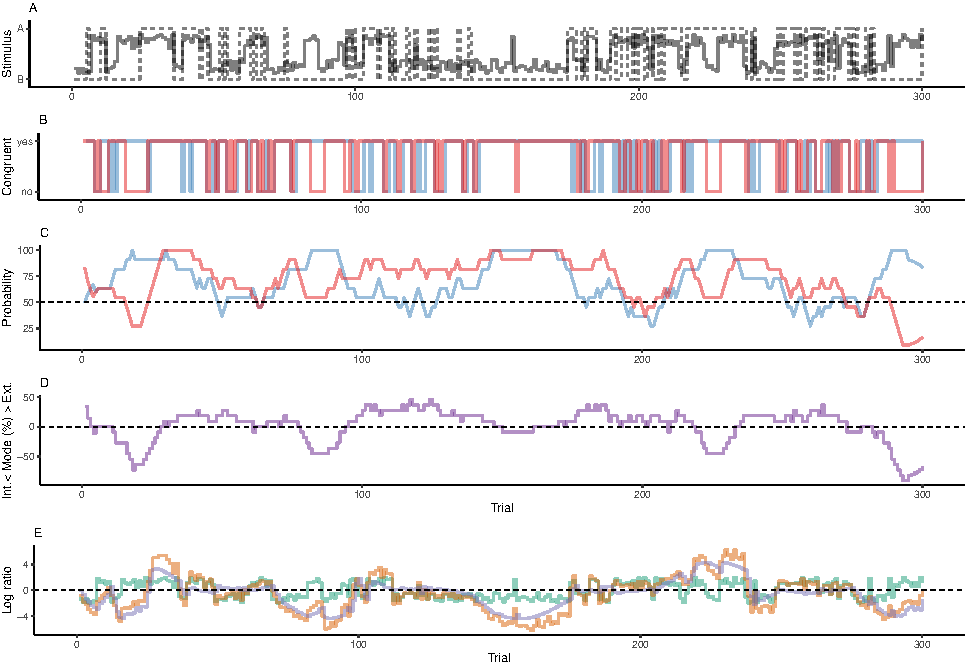
\includegraphics{modes_mouse_files/figure-latex/Figure_1-1.pdf}

\textbf{Figure 1. Concept.}

A. In binary perceptual decision-making, a participant is presented with
stimuli from two categories (A vs.~B; dotted line) and reports
consecutive perceptual choices via button presses (sold line). All
panels below refer to this example data.

B. When the response matched the external stimulus information (i.e.,
overlap between dotted and solid line in panel A), perceptual choices
are \emph{stimulus-congruent} (red line). When the response matches the
response at the preceding trial, perceptual choices are
\emph{history-congruent} (blue line).

C. The dynamic probabilities of stimulus- and history-congruence (i.e.,
computed in sliding windows of ±5 trials) fluctuate over time.

D. The \emph{mode} of perceptual processing is derived by computing the
difference between the dynamic probabilities of stimulus- and
history-congruence. Values above 0\% indicate a bias toward external
information, whereas values below 0\% indicate a bias toward internal
information.

E. In computational modeling, internal mode is caused by an enhanced
impact of perceptual history. This causes the posterior (black line) to
be close to the prior (blue line). Conversely, during external mode, the
posterior is close to the sensory information (log likelihood ratio, red
line).

\newpage

\hypertarget{figure-2}{%
\subsection{Figure 2}\label{figure-2}}

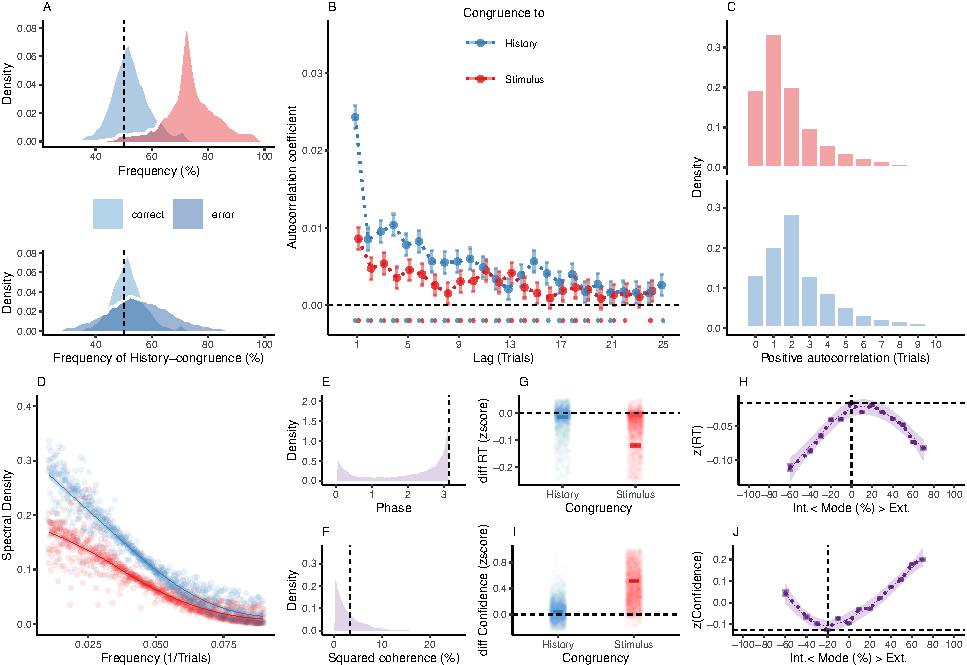
\includegraphics{modes_mouse_files/figure-latex/Figure_2-1.pdf}

\textbf{Figure 2. Internal and external modes in human perceptual
decision-making.}

A. In humans, perception was stimulus-congruent in 73.46\% ± 0.15\% (in
red) and history-congruent in 52.7\% ± 0.12\% of trials (in blue; upper
panel). History-congruent perceptual choices were more frequent when
perception was stimulus-incongruent (i.e., on \emph{error} trials; lower
panel), indicating that history effects impair performance in randomized
psychophysical designs.

B. Relative to randomly permuted data, we found highly significant
autocorrelations of stimulus-congruence and history-congruence (dots
indicate intercepts \(\neq\) 0 in trial-wise linear mixed effects
modeling at p \textless{} 0.05). Across trials, the autocorrelation
coefficients were best fit by an exponential function (adjusted \(R^2\)
for stimulus-congruence: 0.53; history-congruence: 0.71) as compared to
a linear function (adjusted \(R^2\) for stimulus-congruence: 0.52;
history-congruence: 0.49).

C. Here, we depict the number of consecutive trials at which
autocorrelation coefficients exceeded the respective autocorrelation of
randomly permuted data within individual participants. For
stimulus-congruence (upper panel), the lag of positive autocorrelation
amounted to 3.24 ± \ensuremath{2.39\times 10^{-3}} on average, showing a
peak at trial t+1 after the index trial. For history-congruence (lower
panel), the lag of positive autocorrelation amounted to 4.87 ±
\ensuremath{3.36\times 10^{-3}} on average, peaking at trial t+2 after
the index trial.

D. The smoothed probabilities of stimulus- and history-congruence
(sliding windows of ±5 trials) fluctuated as \emph{1/f noise}, i.e., at
power densities that were inversely proportional to the frequency.

E. The distribution of phase shift between fluctuations in stimulus- and
history-congruence peaked at half a cycle (\(\pi\) denoted by dotted
line).

F. The average squared coherence between fluctuations in stimulus- and
history-congruence (black dottet line) amounted to 6.49 ±
\ensuremath{2.07\times 10^{-3}}\%

G. We observed faster response times (RTs) for both stimulus-congruence
(as opposed to stimulus-incongruence, \(\beta\) = \(-0.14\) ±
\(\ensuremath{1.61\times 10^{-3}}\),
T(\(\ensuremath{1.99\times 10^{6}}\)) = \(-85.91\), p < \(\ensuremath{2.2\times 10^{-308}}\)) and
history-congruence (\(\beta\) = \(\ensuremath{-9.73\times 10^{-3}}\) ±
\(\ensuremath{1.38\times 10^{-3}}\),
T(\(\ensuremath{1.99\times 10^{6}}\)) = \(-7.06\), p =
\(\ensuremath{1.66\times 10^{-12}}\)).

H. The mode of perceptual processing (i.e., the difference between the
smoothed probability of stimulus- vs.~history-congruence) showed a
quadratic relationship to RTs, with faster response times for stronger
biases toward both external sensory information and internal predictions
provided by perceptual history (\(\beta_2\) = \(-19.86\) ± \(0.52\),
T(\(\ensuremath{1.98\times 10^{6}}\)) = \(-38.43\), p =
\(\ensuremath{5\times 10^{-323}}\)). The horizontal and vertical dotted
lines indicate maximum RT and the associated mode, respectively.

I. Confidence was enhanced for both stimulus-congruence (as opposed to
stimulus-incongruence, \(\beta\) = \(0.48\) ±
\(\ensuremath{1.38\times 10^{-3}}\),
T(\(\ensuremath{2.06\times 10^{6}}\)) = \(351.89\), p < \(\ensuremath{2.2\times 10^{-308}}\)) and
history-congruence (\(\beta\) = \(0.04\) ±
\(\ensuremath{1.18\times 10^{-3}}\),
T(\(\ensuremath{2.06\times 10^{6}}\)) = \(36.86\), p =
\(\ensuremath{2.93\times 10^{-297}}\)).

J. In analogy to RTs, we found a quadratic relationship between the mode
of perceptual processing and confidence, which increased when both
externally- and internally-biased modes grew stronger (\(\beta_2\) =
\(39.3\) ± \(0.94\), T(\(\ensuremath{2.06\times 10^{6}}\)) = \(41.95\),
p < \(\ensuremath{2.2\times 10^{-308}}\)). The horizontal and vertical dotted lines indicate minimum
confidence and the associated mode, respectively.

\newpage

\hypertarget{figure-3}{%
\subsection{Figure 3}\label{figure-3}}

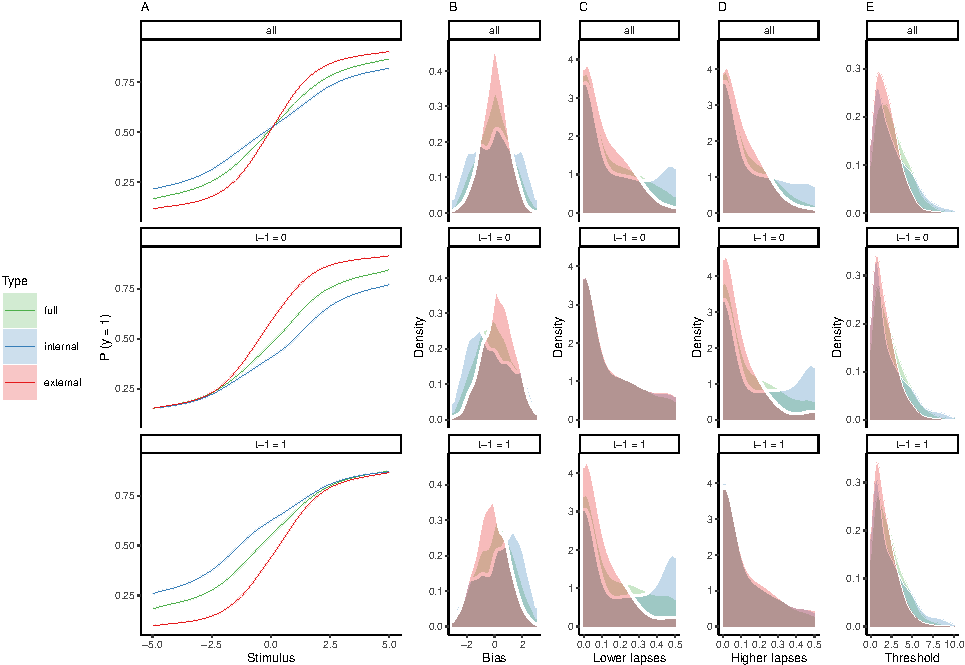
\includegraphics{modes_mouse_files/figure-latex/Figure_3-1.pdf}

\textbf{Figure 3. Full and history-conditioned psychometric functions
across modes in humans.}

A. Here, we show average psychometric functions for the full dataset
(upper panel) and conditioned on perceptual history (\(y_{t-1} = 1\) and
\(y_{t-1} = 0\); middle and lower panel) across modes (green line) and
for internal mode (blue line) and external mode (red line) separately.

B. Across the full dataset, biases \(\mu\) were distributed around zero
(\(\beta_0\) = \(\ensuremath{7.37\times 10^{-3}}\) ± \(0.09\),
T(\(36.8\)) = \(0.08\), p = \(0.94\); upper panel), with larger absolute
biases \(|\mu|\) for internal as compared to external mode (\(\beta_0\)
= \(-0.62\) ± \(0.07\), T(\(45.62\)) = \(-8.38\), p =
\(\ensuremath{8.59\times 10^{-11}}\); controlling for differences in
lapses and thresholds). When conditioned on perceptual history, we
observed negative biases for \(y_{t-1} = 0\) (\(\beta_0\) = \(0.56\) ±
\(0.12\), T(\(43.39\)) = \(4.6\), p =
\(\ensuremath{3.64\times 10^{-5}}\); middle panel) and positive biases
for \(y_{t-1} = 1\) (\(\beta_0\) = \(0.56\) ± \(0.12\), T(\(43.39\)) =
\(4.6\), p = \(\ensuremath{3.64\times 10^{-5}}\); lower panel).

C. Lapse rates were higher in internal mode as compared to external mode
(\(\beta_0\) = \(-0.05\) ± \(\ensuremath{5.73\times 10^{-3}}\),
T(\(47.03\)) = \(-9.11\), p = \(\ensuremath{5.94\times 10^{-12}}\);
controlling for differences in biases and thresholds; see upper panel
and subplot D). Importantly, the between-mode difference in lapses
depended on perceptual history: We found no significant difference in
lower lapses \(\gamma\) for \(y_{t-1} = 0\) (\(\beta_0\) = \(0.01\) ±
\(\ensuremath{7.77\times 10^{-3}}\), T(\(33.1\)) = \(1.61\), p =
\(0.12\); middle panel), but a significant difference for
\(y_{t-1} = 1\) (\(\beta_0\) = \(-0.11\) ± \(0.01\), T(\(40.11\)) =
\(-9.59\), p = \(\ensuremath{6.14\times 10^{-12}}\); lower panel).

D. Conversely, higher lapses \(\delta\) were significantly increased for
\(y_{t-1} = 0\) (\(\beta_0\) = \(-0.1\) ±
\(\ensuremath{9.58\times 10^{-3}}\), T(\(36.87\)) = \(-10.16\), p =
\(\ensuremath{3.06\times 10^{-12}}\); middle panel), but not for
\(y_{t-1} = 1\) (\(\beta_0\) = \(0.01\) ±
\(\ensuremath{7.74\times 10^{-3}}\), T(\(33.66\)) = \(1.58\), p =
\(0.12\); lower panel).

E. The thresholds \(t\) were larger in internal as compared to external
mode (\(\beta_0\) = \(-1.77\) ± \(0.25\), T(\(50.45\)) = \(-7.14\), p =
\(\ensuremath{3.48\times 10^{-9}}\); controlling for differences in
biases and lapses) and were not modulated by perceptual history
(\(\beta_0\) = \(0.04\) ± \(0.06\),
T(\(\ensuremath{2.97\times 10^{3}}\)) = \(0.73\), p = \(0.47\)).

\newpage

\hypertarget{figure-4}{%
\subsection{Figure 4}\label{figure-4}}

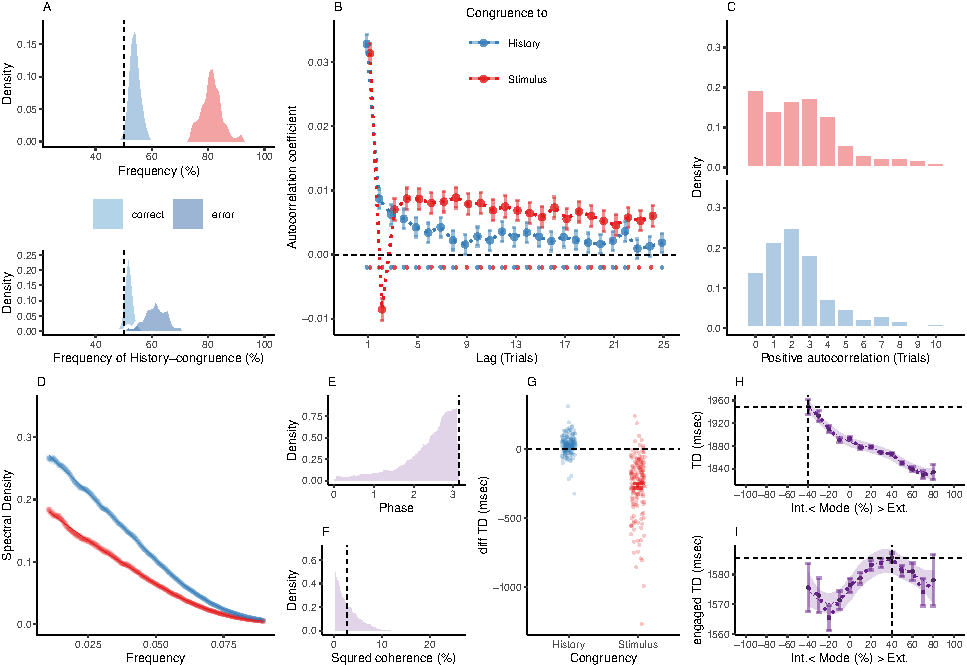
\includegraphics{modes_mouse_files/figure-latex/Figure_4-1.pdf}

\textbf{Figure 4. Internal and external modes in murine perceptual
decision-making.}

A. In mice, 81.37\% ± 0.3\% of trials were stimulus-congruent (in red)
and 54.03\% ± 0.17\% of trials were history-congruent (in blue; upper
panel). History-congruent perceptual choices were not a consequence of
the experimental design, but a source of error, as they were more
frequent on stimulus-incongruent trials (lower panel).

B. Relative to randomly permuted data, we found highly significant
autocorrelations of stimulus-congruence and history-congruence (dots
indicate intercepts \(\neq\) 0 in trial-wise linear mixed effects
modeling at p \textless{} 0.05). Please note that the negative
autocorrelation of stimulus-congruence at trial 2 was a consequence of
the experimental design (see Supplemental Figure 2D-F). As in humans,
autocorrelation coefficients were best fit by an exponential function
(adjusted \(R^2\) for stimulus-congruence: 0.44; history-congruence:
0.52) as compared to a linear function (adjusted \(R^2\) for
stimulus-congruence: \ensuremath{3.16\times 10^{-3}};
history-congruence: 0.26).

C. For stimulus-congruence (upper panel), the lag of positive
autocorrelation was longer in comparison to humans (4.59 ± 0.06 on
average). For history-congruence (lower panel), the lag of positive
autocorrelation was slightly shorter relative to humans (2.58 ± 0.01 on
average, peaking at trial t+2 after the index trial).

D. In mice, the dynamic probabilities of stimulus- and
history-congruence (sliding windows of ±5 trials) fluctuated as
\emph{1/f noise}.

E. The distribution of phase shift between fluctuations in stimulus- and
history-congruence peaked at half a cycle (\(\pi\) denoted by dotted
line).

F. The average squared coherence between fluctuations in stimulus- and
history-congruence (black dottet line) amounted to 3.45 ± 0.01\%

G. We observed shorter trial durations (TDs) for stimulus-congruence (as
opposed to stimulus-incongruence, \(\beta\) = \(-1.12\) ±
\(\ensuremath{8.53\times 10^{-3}}\),
T(\(\ensuremath{1.34\times 10^{6}}\)) = \(-131.78\), p < \(\ensuremath{2.2\times 10^{-308}}\)), but
longer TDs for history-congruence (\(\beta\) = \(0.06\) ±
\(\ensuremath{6.76\times 10^{-3}}\),
T(\(\ensuremath{1.34\times 10^{6}}\)) = \(8.52\), p =
\(\ensuremath{1.58\times 10^{-17}}\)).

H. TDs decreased monotonically for stronger biases toward external mode
(\(\beta_1\) = \(\ensuremath{-4.16\times 10^{4}}\) ±
\(\ensuremath{1.29\times 10^{3}}\),
T(\(\ensuremath{1.35\times 10^{6}}\)) = \(-32.31\), p =
\(\ensuremath{6.03\times 10^{-229}}\)). The horizontal and vertical
dotted lines indicate maximum TD and the associated mode, respectively.

I. For TDs that differed from the median TD by no more than 1.5 x MAD
(median absolute distance\textsuperscript{52}), mice exhibited a
quadratic component in the relationship between the mode of sensory
processing and TDs (\(\beta_2\) = \(\ensuremath{-1.97\times 10^{3}}\) ±
\(843.74\), T(\(\ensuremath{1.19\times 10^{6}}\)) = \(-2.34\), p =
\(0.02\), Figure 4I). This explorative post-hoc analysis focuses on
trials at which mice engage more swiftly with the experimental task. The
horizontal and vertical dotted lines indicate maximum TD and the
associated mode, respectively.

\newpage

\hypertarget{figure-5}{%
\subsection{Figure 5}\label{figure-5}}

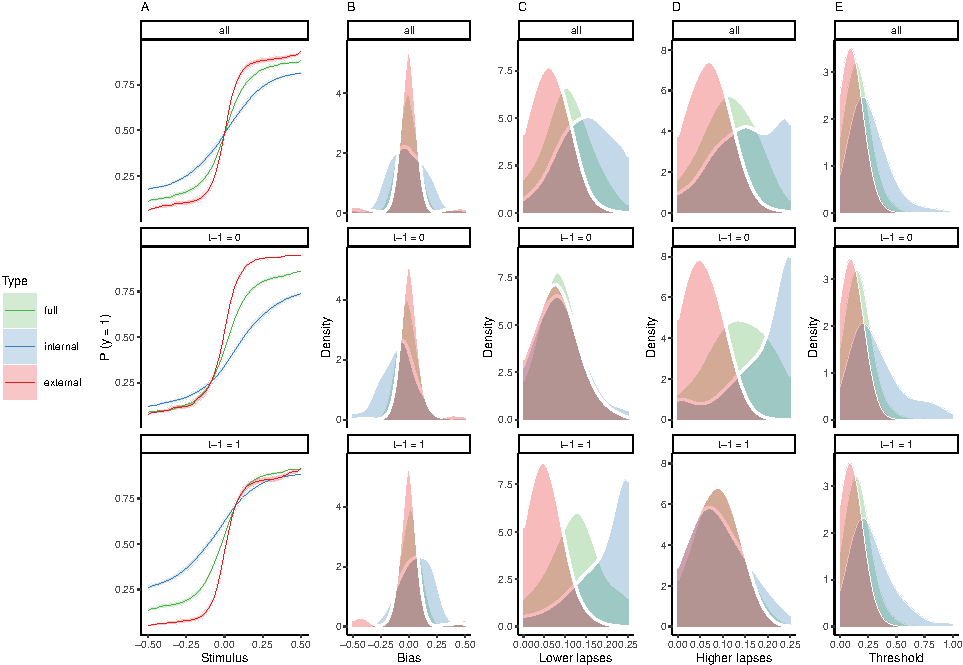
\includegraphics{modes_mouse_files/figure-latex/Figure_5-1.pdf}

\textbf{Figure 5. Full and history-conditioned psychometric functions
across modes in mic.}

A. Here, we show average psychometric functions for the full IBL dataset
(upper panel) and conditioned on perceptual history (\(y_{t-1} = 1\) and
\(y_{t-1} = 0\); middle and lower panel) across modes (green line) and
for internal mode (blue line) and external mode (red line) separately.

B. Across the full dataset, biases \(\mu\) were distributed around zero
(T(164) = 0.39, p = \(0.69\); upper panel), with larger absolute biases
\(|\mu|\) for internal as compared to external mode (\(\beta_0\) =
\(-0.18\) ± \(0.03\), T = \(-6.38\), p =
\(\ensuremath{1.77\times 10^{-9}}\); controlling for differences in
lapses and thresholds). When conditioned on perceptual history, we
observed negative biases for \(y_{t-1} = 0\) (T(164) = -1.99, p =
\(0.05\); middle panel) and positive biases for \(y_{t-1} = 1\) (T(164)
= 1.91, p = \(0.06\); lower panel).

C. Lapse rates were higher in internal as compared to external mode
(\(\beta_0\) = \(-0.11\) ± \(\ensuremath{4.39\times 10^{-3}}\), T =
\(-24.8\), p = \(\ensuremath{4.91\times 10^{-57}}\); controlling for
differences in biases and thresholds; upper panel, see also subplot D).
For \(y_{t-1} = 1\), the difference between internal and external mode
was more pronounced for lower lapses \(\gamma\) (T(164) = -18.24, p =
\(\ensuremath{2.68\times 10^{-41}}\)) as compared to higher lapses
\(\delta\) (see subplot D). In mice, lower lapses \(\gamma\) were
significantly elevated during internal mode irrespective of the
preceding perceptual choice (middle panel: lower lapses \(\gamma\) for
\(y_{t-1} = 0\); T(164) = -2.5, p = \(0.01\), lower panel: lower lapses
\(\gamma\) for \(y_{t-1} = 1\); T(164) = -32.44, p =
\(\ensuremath{2.92\times 10^{-73}}\)).

D. For \(y_{t-1} = 0\), the difference between internal and external
mode was more pronounced for higher lapses \(\delta\) (T(164) = 21.44, p
= \(\ensuremath{1.93\times 10^{-49}}\), see subplot C). Higher lapses
were significantly elevated during internal mode irrespective of the
preceding perceptual choice (middle panel: higher lapses \(\delta\) for
\(y_{t-1} = 0\); T(164) = -28.29, p =
\(\ensuremath{5.62\times 10^{-65}}\) lower panel: higher lapses
\(\delta\) for \(y_{t-1} = 1\); T(164) = -2.65, p =
\(\ensuremath{8.91\times 10^{-3}}\); ).

E. Thresholds \(t\) were higher in internal as compared to external mode
(\(\beta_0\) = \(-0.28\) ± \(0.04\), T = \(-7.26\), p =
\(\ensuremath{1.53\times 10^{-11}}\); controlling for differences in
biases and lapses) and were not modulated by perceptual history (T(164)
= 0.94, p = \(0.35\)).

\newpage

\hypertarget{figure-6}{%
\subsection{Figure 6}\label{figure-6}}

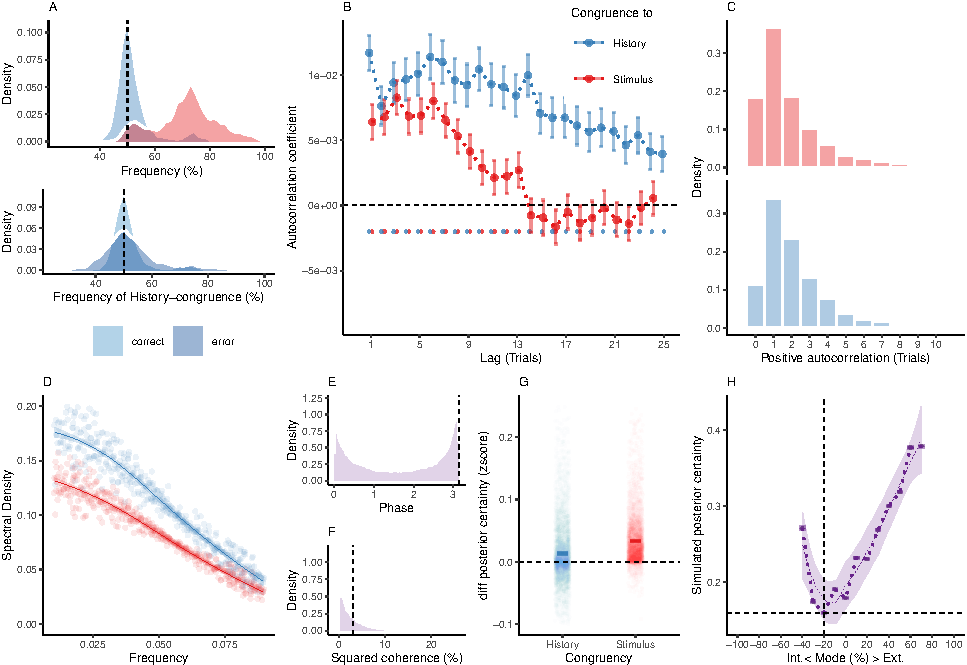
\includegraphics{modes_mouse_files/figure-latex/Figure_6-1.pdf}

\textbf{Figure 6. Internal and external modes in simulated perceptual
decision-making.}

A. Simulated perceptual choices were stimulus-congruent in 71.36\% ±
0.17\% (in red) and history-congruent in 51.99\% ± 0.11\% of trials (in
blue; T(\ensuremath{4.32\times 10^{3}}) = 17.42, p =
\(\ensuremath{9.89\times 10^{-66}}\); upper panel). Due to the
competition between stimulus- and history-congruence, history-congruent
perceptual choices were more frequent when perception was
stimulus-incongruent (i.e., on \emph{error} trials;
T(\ensuremath{4.32\times 10^{3}}) = 11.19, p =
\(\ensuremath{1.17\times 10^{-28}}\); lower panel) and thus impaired
performance in the randomized psychophysical design simulated here.

B. At the simulated group level, we found significant autocorrelations
in both stimulus-congruence (13 consecutive trials) and
history-congruence (30 consecutive trials).

C. On the level of individual simulated participants, autocorrelation
coefficients exceeded the autocorrelation coefficients of randomly
permuted data within a lag of 2.46 ± \ensuremath{1.17\times 10^{-3}}
trials for stimulus-congruence and 4.24 ±
\ensuremath{1.85\times 10^{-3}} trials for history-congruence.

D. The smoothed probabilities of stimulus- and history-congruence
(sliding windows of ±5 trials) fluctuated as \emph{1/f noise}, i.e., at
power densities that were inversely proportional to the frequency (power
\textasciitilde{} 1/\(f^\beta\); stimulus-congruence: \(\beta\) =
\(-0.81\) ± \(\ensuremath{1.18\times 10^{-3}}\),
T(\(\ensuremath{1.92\times 10^{5}}\)) = \(-687.58\), p < \(\ensuremath{2.2\times 10^{-308}}\);
history-congruence: \(\beta\) = \(-0.83\) ±
\(\ensuremath{1.27\times 10^{-3}}\),
T(\(\ensuremath{1.92\times 10^{5}}\)) = \(-652.11\), p < \(\ensuremath{2.2\times 10^{-308}}\)).

E. The distribution of phase shift between fluctuations in simulated
stimulus- and history-congruence peaked at half a cycle (\(\pi\) denoted
by dotted line). The dynamic probabilities of simulated stimulus- and
history-congruence were therefore were strongly anti-correlated
(\(\beta\) = \(-0.03\) ± \(\ensuremath{8.22\times 10^{-4}}\),
T(\(\ensuremath{2.12\times 10^{6}}\)) = \(-40.52\), p < \(\ensuremath{2.2\times 10^{-308}}\)).

F. The average squared coherence between fluctuations in simulated
stimulus- and history-congruence (black dotted line) amounted to 6.49 ±
\ensuremath{2.07\times 10^{-3}}\%.

G. Simulated confidence was enhanced for stimulus-congruence (\(\beta\)
= \(0.03\) ± \(\ensuremath{1.71\times 10^{-4}}\),
T(\(\ensuremath{2.03\times 10^{6}}\)) = \(178.39\), p < \(\ensuremath{2.2\times 10^{-308}}\)) and
history-congruence (\(\beta\) = \(0.01\) ±
\(\ensuremath{1.5\times 10^{-4}}\),
T(\(\ensuremath{2.03\times 10^{6}}\)) = \(74.18\), p < \(\ensuremath{2.2\times 10^{-308}}\)).

H. In analogy to humans, the simulated data showed a quadratic
relationship between the mode of perceptual processing and posterior
certainty, which increased for stronger external and internal biases
(\(\beta_2\) = \(31.03\) ± \(0.15\),
T(\(\ensuremath{2.04\times 10^{6}}\)) = \(205.95\), p < \(\ensuremath{2.2\times 10^{-308}}\)). The
horizontal and vertical dotted lines indicate minimum posterior
certainty and the associated mode, respectively.

\newpage

\hypertarget{figure-7}{%
\subsection{Figure 7}\label{figure-7}}

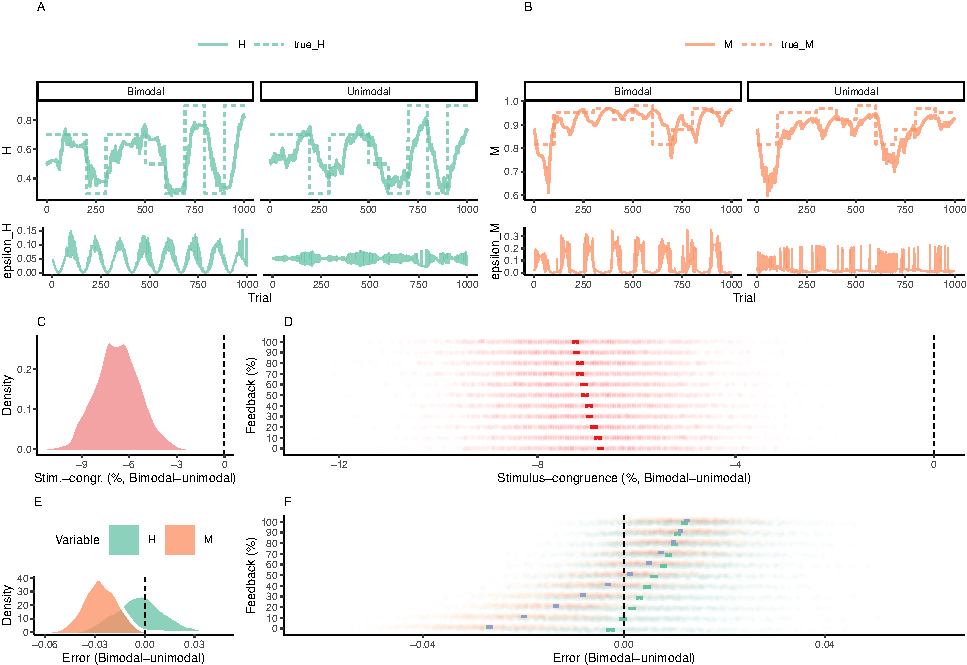
\includegraphics{modes_mouse_files/figure-latex/Figure_7-1.pdf}

\textbf{Figure 7. Adaptive benefits of bimodal inference.}

A. When the sensory environment changes unpredictably over time, agents
have to update estimates \(H_t\) (solid green line, upper panel) about
the true hazard rate \(\hat{H_t}\) from experience (dotted green line,
upper panel). Updates to \(H_t\) are driven by an error term
\(\epsilon_H\) (solid green line, lower panel) that is defined by the
difference between \(H_t\) and the presence of a perceived change in the
environment. In contrast to the unimodal model (right panels),
\(\epsilon_H\) of the bimodal model (left panels) is modulated by a
phasic component reflecting ongoing fluctuations between internal and
external mode.

B. When the precision of sensory encoding changes unpredictably over
time, agents have to update estimates \(M_t\) (solid orange line, upper
panel) about the true precision of sensory encoding \(\hat{M_t}\) from
experience (dotted orange line, upper panel). Updates to \(M_t\) are
driven by an error term \(\epsilon_M\) (red line, lower panel) that is
defined by the difference between \(M_t\) and the posterior
decision-certainty. In contrast to the unimodal model (right panels),
\(\epsilon_M\) of the bimodal model (left panels) is modulated by a
phasic component reflecting ongoing fluctuations between internal and
external mode.

C. In the absence of feedback, the bimodal inference model achieved
lower stimulus-congruence as compared the unimodal control model
(\(\beta_1\) = \(-6.71\) ± \(0.03\),
T(\(\ensuremath{8.42\times 10^{3}}\)) = \(-234.31\), p < \(\ensuremath{2.2\times 10^{-308}}\)).

D. The unimodal control model benefited more strongly from the presence
of external feedback, leading to a relative decrease in
stimulus-congruence for the bimodal inference model at higher feedback
levels (\(\beta_2\) = \(-0.05\) ± \(\ensuremath{4.13\times 10^{-3}}\),
T(\(\ensuremath{10\times 10^{3}}\)) = \(-12.32\), p =
\(\ensuremath{1.25\times 10^{-34}}\)).

E. In the absence of feedback, the bimodal inference model achieved
lower errors in the estimated hazard rate \(H\) (\(\beta_1\) =
\(\ensuremath{-2.94\times 10^{-3}}\) ±
\(\ensuremath{2.89\times 10^{-4}}\),
T(\(\ensuremath{4.96\times 10^{3}}\)) = \(-10.18\), p =
\(\ensuremath{4.11\times 10^{-24}}\)) as well as lower errors in the
estimated probability of stimulus-congruent choices \(M\) (\(\beta_1\) =
\(-0.03\) ± \(\ensuremath{1.86\times 10^{-4}}\),
T(\(\ensuremath{6.07\times 10^{3}}\)) = \(-137.75\), p < \(\ensuremath{2.2\times 10^{-308}}\)).

F. With an increasing availability of feedback, the advantage of the
bimodal inference model was lost with respect to \(H\) (\(\beta_2\) =
\(\ensuremath{1.43\times 10^{-3}}\) ±
\(\ensuremath{3.71\times 10^{-5}}\), T(\(\ensuremath{10\times 10^{3}}\))
= \(38.58\), p = \(\ensuremath{9.44\times 10^{-304}}\)) and \(M\)
(\(\beta_2\) = \(\ensuremath{3.91\times 10^{-3}}\) ±
\(\ensuremath{2.51\times 10^{-5}}\), T(\(\ensuremath{10\times 10^{3}}\))
= \(156.18\), p < \(\ensuremath{2.2\times 10^{-308}}\)).

\newpage

\hypertarget{supplemental-items}{%
\section{Supplemental Items}\label{supplemental-items}}

\hypertarget{supplemental-figure-s1}{%
\subsection{Supplemental Figure S1}\label{supplemental-figure-s1}}

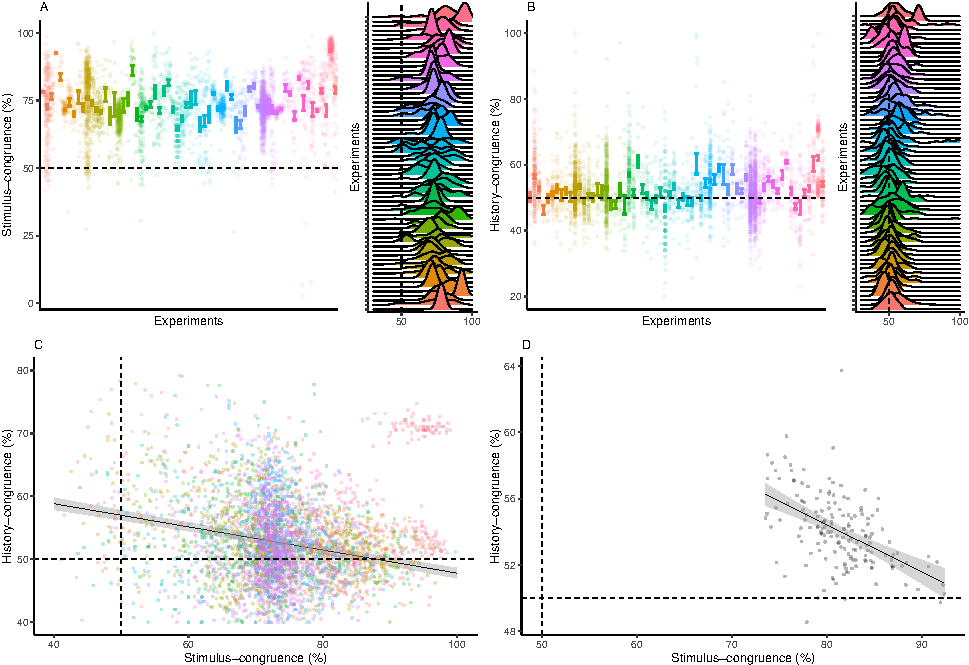
\includegraphics{modes_mouse_files/figure-latex/Supplememtal_Figure_S1-1.pdf}

\textbf{Supplemental Figure S1. Stimulus- and history-congruence.}

A. Stimulus-congruent choices in humans amounted to 73.46\% ± 0.15\% of
trials and were highly consistent across the experiments selected from
the Confidence Database.

B. History-congruent choices in humans amounted to 52.7\% ± 0.12\% of
trials. In analogy to stimulus-congruence, the prevalence of
history-congruence was highly consistent across the experiments selected
from the Confidence Database. 48.48\% of experiments showed significant
(p \textless{} 0.05) attractive biases toward preceding choices, whereas
3.03\% of experiments showed significant repulsive biases.

C. In humans, we found an enhanced impact of perceptual history in
participants who were less sensitive to external sensory information
(T(\(\ensuremath{4.3\times 10^{3}}\)) = \(-14.27\), p =
\(\ensuremath{3.78\times 10^{-45}}\)), suggesting that perception
results from the competition of external with internal information.

D. In analogy to humans, mice that were less sensitive to external
sensory information showed stronger biases toward perceptual history
(T(163) = -7.52, p = \(\ensuremath{3.44\times 10^{-12}}\), Pearson
correlation).

\newpage

\hypertarget{supplemental-figure-s2}{%
\subsection{Supplemental Figure S2}\label{supplemental-figure-s2}}

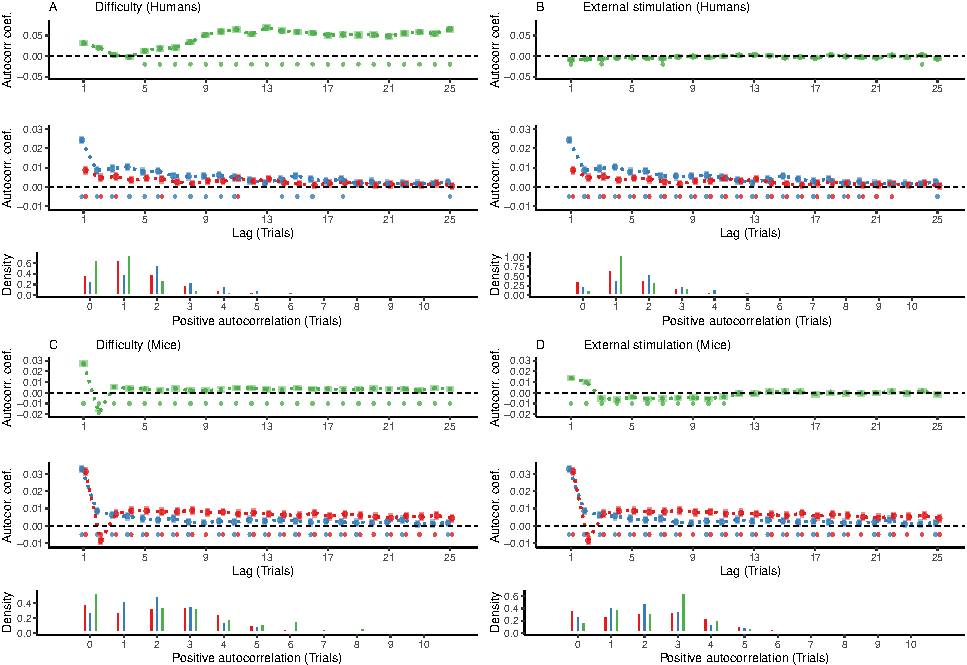
\includegraphics{modes_mouse_files/figure-latex/Supplememtal_Figure_S2-1.pdf}

\textbf{Supplemental Figure S2. Controlling for task difficulty and
external stimulation.}

In this study, we found highly significant autocorrelations of stimulus-
and history-congruence in humans as well as in mice. Here, we show that
these autocorrelations are not a trivial consequence of task difficulty
or the sequence external stimulation. In addition, we computed
trial-wise logistic regression coefficients as an alternative approach
to assessing serial dependencies in stimulus- and history-congruence.

A. In humans, task difficulty (in green) showed a significant
autocorrelated starting at the 5th trial (upper panel, dots at the
bottom indicate intercepts \(\neq\) 0 in trial-wise linear mixed effects
modeling at p \textless{} 0.05). When controlling for task difficulty,
linear mixed effects modeling indicated a significant auto-correlation
of stimulus-congruence (in red) for the first 3 consecutive trials
(middle panel). 20\% of trials within the displayed time window remained
significantly autocorrelated. The autocorrelation of history-congruence
(in blue) remained significant for the first 11 consecutive trials (64\%
significantly autocorrelated trials within the displayed time window).
At the level of individual participants, the autocorrelation of task
difficulty exceeded the respective autocorrelation of randomly permuted
within a lag of 21.66 ± \ensuremath{8.37\times 10^{-3}} trials (lower
panel).

B. The sequence of external stimulation (i.e., which of the two binary
outcomes was supported by the presented stimuli; depicted in green) was
negatively autocorrelated for 1 trial. When controlling for the
autocorrelation of external stimulation, stimulus-congruence remained
significantly autocorrelated for 22 consecutive trials (88\% of trials
within the displayed time window; lower panel) and history-congruence
remained significantly autocorrelated for 20 consecutive trials (84\% of
trials within the displayed time window). At the level of individual
participants, the autocorrelation of external stimulation exceeded the
respective autocorrelation of randomly permuted within a lag of 2.94 ±
\ensuremath{4.4\times 10^{-3}} consecutive trials (lower panel).

D. In mice, task difficulty showed an significant autocorrelated for the
first 25 consecutive trials (upper panel). When controlling for task
difficulty, linear mixed effects modeling indicated a significant
auto-correlation of stimulus-congruence for the first 36 consecutive
trials (middle panel). In total, 100\% of trials within the displayed
time window remained significantly autocorrelated. The autocorrelation
of history-congruence remained significant for the first 8 consecutive
trials, with 84\% significantly autocorrelated trials within the
displayed time window. At the level of individual mice, autocorrelation
coefficients for difficulty were elevated above randomly permuted data
within a lag of 15.13 ± 0.19 consecutive trials (lower panel).

E. In mice, the sequence of external stimulation (i.e., which of the two
binary outcomes was supported by the presented stimuli) was negatively
autocorrelated for 11 consecutive trials (upper panel). When controlling
for the autocorrelation of external stimulation, stimulus-congruence
remained significantly autocorrelated for 86 consecutive trials (100\%
of trials within the displayed time window; middle) and
history-congruence remained significantly autocorrelated for 8
consecutive trials (84\% of trials within the displayed time window). At
the level of individual mice, autocorrelation coefficients for external
stimulation were elevated above randomly permuted data within a lag of
2.53 ± \ensuremath{9.8\times 10^{-3}} consecutive trials (lower panel).

\newpage

\hypertarget{supplemental-figure-s3}{%
\subsection{Supplemental Figure S3}\label{supplemental-figure-s3}}

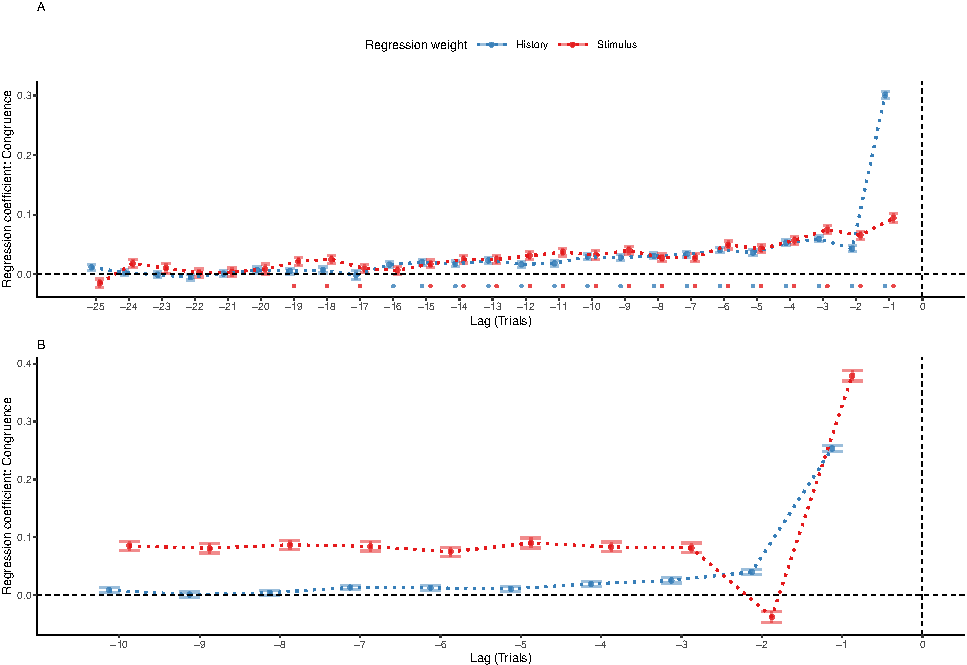
\includegraphics{modes_mouse_files/figure-latex/Supplememtal_Figure_S3-1.pdf}

\textbf{Supplemental Figure S3. Reproducing group-level autocorrelations
using logistic regression.}

A. As an alternative to group-level autocorrelation coefficients, we
used trial-wise logistic regression to quantify serial dependencies in
stimulus- and history-congruence. This analysis predicted stimulus- and
history-congruence at the index trial (trial \(t = 0\), vertical line)
based on stimulus- and history-congruence at the 25 preceding trials.
Mirroring the shape of the group-level autocorrelations, trial-wise
regression coefficients (depicted as mean ± SEM, dots mark trials with
regression weights significantly greater than zero at p \textless{}
0.05) increased toward the index trial \(t = 0\) for the human data.

B. Following our results in human data, regression coefficients that
predicted history-congruence at the index trial (trial t = 0, vertical
line) increased exponentially for trials closer to the index trial in
mice. In contrast to history-congruence, stimulus-congruence showed a
negative regression weight (or autocorrelation coefficient, see Figure
4B) at trial -2. This was due to the experimental design (see also the
autocorrelations of difficulty and external stimulation in Supplemental
Figure S2C and D): When mice made errors at easy trials (contrast
\(\geq\) 50\%), the upcoming stimulus was shown at the same spatial
location and at high contrast. This increased the probability of
stimulus-congruent perceptual choices after stimulus-incongruent
perceptual choices at easy trials, thereby creating a negative
regression weight (or autocorrelation coefficient) of
stimulus-congruence at trial -2.

\newpage

\hypertarget{supplemental-figure-s4}{%
\subsection{Supplemental Figure S4}\label{supplemental-figure-s4}}

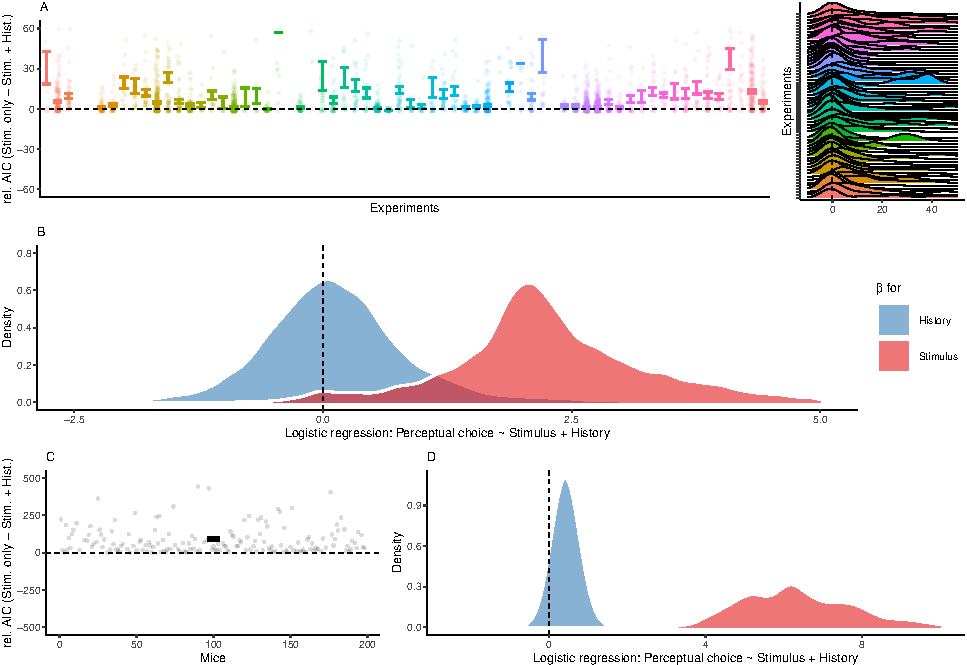
\includegraphics{modes_mouse_files/figure-latex/Supplememtal_Figure_S4-1.pdf}

\textbf{Supplemental Figure S4. History-congruence in logistic
regression.}

A. To ensure that perceptual history played a significant role in
perception despite the ongoing stream of external information, we tested
whether human perceptual decision-making was better explained by the
combination of external and internal information or, alternatively, by
external information alone. To this end, we compared Aikake information
criteria between logistic regression models that predicted trial-wise
perceptual responses either by both current external sensory information
and the preceding percept, or by external sensory information alone
(values above zero indicate a superiority of the full model). With high
consistency across the experiments selected from the Confidence
Database, this model-comparison confirmed that perceptual history
contributed significantly to perception (difference in AIC = 8.07 ±
0.53, T(\(57.22\)) = \(4.1\), p = \(\ensuremath{1.31\times 10^{-4}}\)).

B. Participant-wise regression coefficients amount to 0.18 ± 0.02 for
the effect of perceptual history and 2.51 ± 0.03 for external sensory
stimulation.

C. In mice, an AIC-based model comparison indicated that perception was
better explained by logistic regression models that predicted trial-wise
perceptual responses based on both current external sensory information
and the preceding percept (difference in AIC = 88.62 ± 8.57, T(\(164\))
= \(-10.34\), p = \(\ensuremath{1.29\times 10^{-19}}\)).

D. In mice, individual regression coefficients amounted to 0.42 ± 0.02
for the effect of perceptual history and 6.91 ± 0.21 for external
sensory stimulation.

\newpage

\hypertarget{supplemental-figure-s5}{%
\subsection{Supplemental Figure S5}\label{supplemental-figure-s5}}

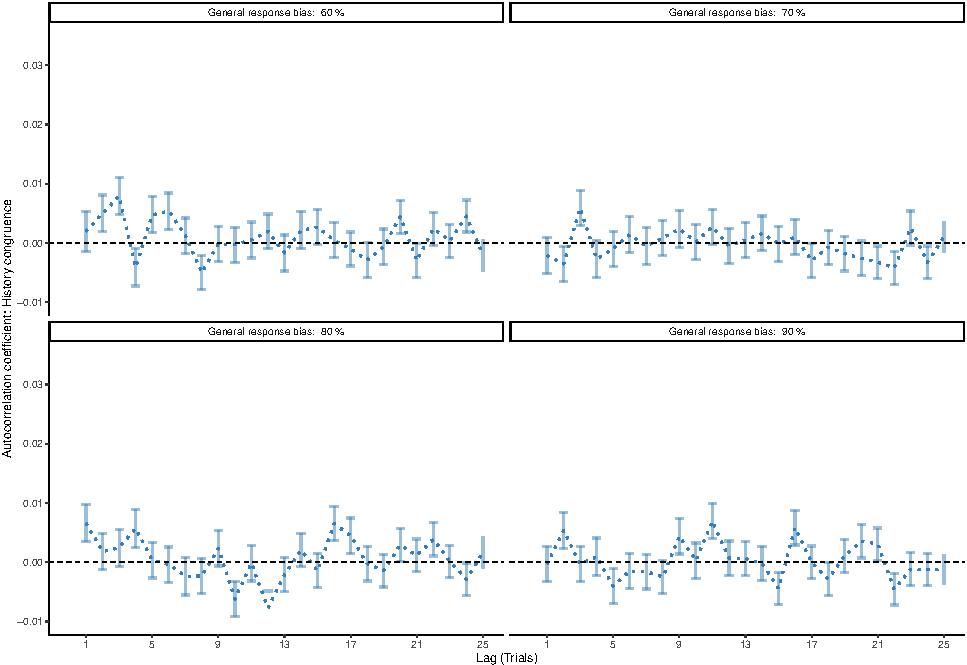
\includegraphics{modes_mouse_files/figure-latex/Supplemental_Figure_S5-1.pdf}

\textbf{Supplemental Figure S5. Correcting for general response biases.}

Here, we ask whether the autocorrelation of history-congruence (as shown
in Figure 2-3C) may be driven by general response biases (i.e., a
general propensity to choose one of the two possible outcomes more
frequently than the alternative). To this end, we generated sequences of
100 perceptual choices with general response biases ranging from 60 to
90\% for 1000 simulated participants each. We then computed the
autocorrelation of history-congruence for these simulated data.
Crucially, we used the correction procedure that is applied to all
autocorrelation curves shown in this manuscript: All reported
autocorrelation coefficients are computed relative to the average
autocorrelation coefficients obtained for 100 iterations of randomly
permuted trial sequences. The above simulation show that this correction
procedure removes any potential contribution of general response biases
to the auto-correlation of history-congruence. This indicates that the
autocorrelation of history-congruence (as shown in Figure 2-3C) is not
driven by general response biases that were present in the empirical
data at a level of 58.71\% ± 0.22\% in humans and 54.6\% ± 0.3\% in
mice.

\newpage

\hypertarget{supplemental-figure-s6}{%
\subsection{Supplemental Figure S6}\label{supplemental-figure-s6}}

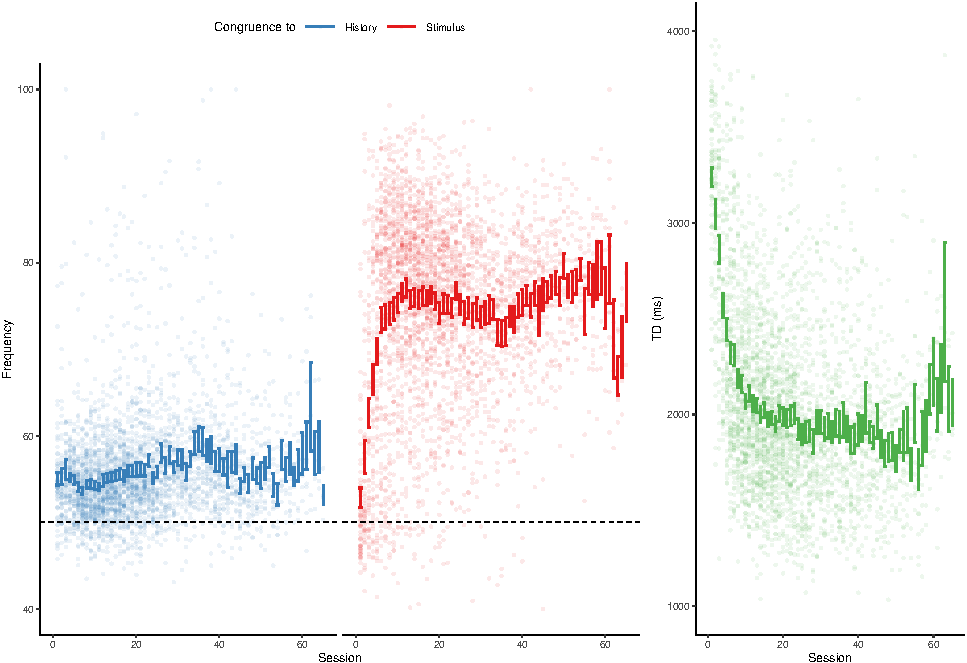
\includegraphics{modes_mouse_files/figure-latex/Supplemental_Figure_S6-1.pdf}

\textbf{Supplemental Figure S6. History-/stimulus-congruence and TDs
during training of the basic task.}

Here, we depict the progression of history- and stimulus-congruence
(depicted in blue and red, respectively; left panel) as well as TDs (in
green; right panel) across training sessions in mice that achieved
proficiency (i.e., stimulus-congruence \(\geq\) 80\%) in the
\emph{basic} task of the IBL dataset. We found that both
history-congruent perceptual choices (\(\beta\) = \(0.13\) ±
\(\ensuremath{4.67\times 10^{-3}}\),
T(\(\ensuremath{8.4\times 10^{3}}\)) = \(27.04\), p =
\(\ensuremath{1.96\times 10^{-154}}\)) and stimulus-congruent perceptual
choices (\(\beta\) = \(0.34\) ± \(\ensuremath{7.13\times 10^{-3}}\),
T(\(\ensuremath{8.51\times 10^{3}}\)) = \(47.66\), p < \(\ensuremath{2.2\times 10^{-308}}\)) became
more frequent with training. As in humans, mice showed shorter TDs with
increase exposure to the task (\(\beta\) = \(-22.14\) ± \(17.06\),
T(\(\ensuremath{1.14\times 10^{3}}\)) = \(-1.3\), p < \(\ensuremath{2.2\times 10^{-308}}\)).

\newpage

\hypertarget{supplemental-figure-s7}{%
\subsection{Supplemental Figure S7}\label{supplemental-figure-s7}}

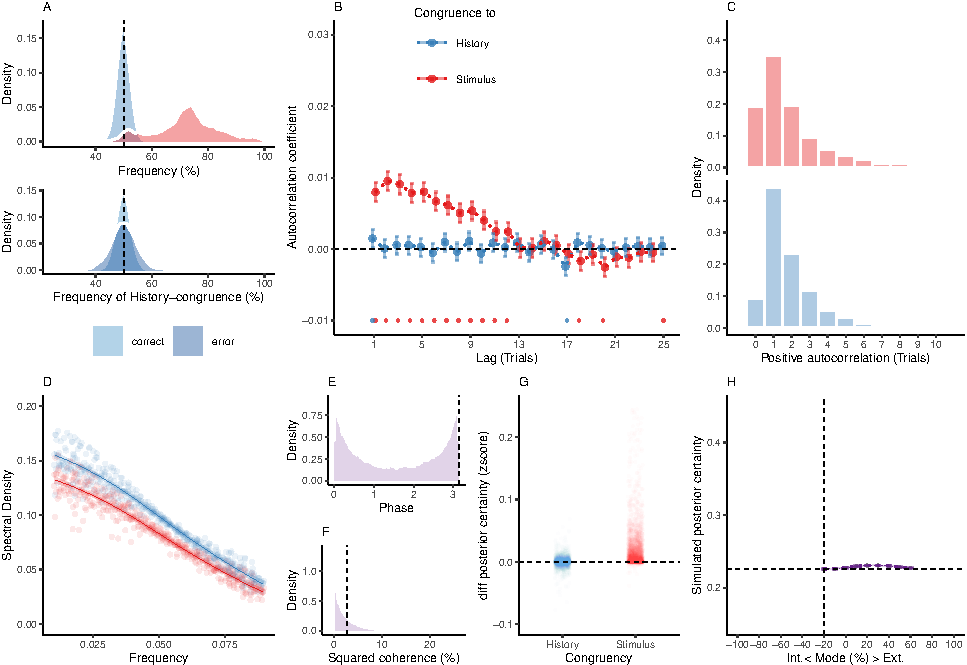
\includegraphics{modes_mouse_files/figure-latex/Supplemental_Figure_S7-1.pdf}

\textbf{Supplemental Figure S7. Reduced Control Model 1: No accumulation
of information across trials.} When simulating data for the
\emph{no-accumulation model}, we removed the accumulation of information
across trials by setting the Hazard rate \(H\) to 0.5. Simulated data
thus depended only on the participant-wise estimates for the amplitudes
\(a_{LLR/\psi}\), frequency \(f\), phase \(p\) and inverse decision
temperature \(\zeta\).

A. Similar to the full model (Figure 6), simulated perceptual choices
were stimulus-congruent in 72.14\% ± 0.17\% of trials (in red).
History-congruent amounted to 49.89\% ± 0.03\% of trials (in blue). In
contrast to the full model, the no-accumulation model showed a
significant bias against perceptual history
T(\ensuremath{4.32\times 10^{3}}) = -3.28, p =
\(\ensuremath{1.06\times 10^{-3}}\); upper panel). In contrast to the
full model, there was no difference in the frequency of
history-congruent choices between correct and error trials
(T(\ensuremath{4.31\times 10^{3}}) = 0.76, p = \(0.44\); lower panel).

B. In the no-accumulation model, we found no significant autocorrelation
of history-congruence beyond the first trial, whereas the
autocorrelation of stimulus-congruence was preserved.

C. In the no-accumulation model, the number of consecutive trials at
which true autocorrelation coefficients exceeded the autocorrelation
coefficients for randomly permuted data increased with respect to
stimulus-congruence (2.83 ± \ensuremath{1.49\times 10^{-3}} trials;
T(\ensuremath{4.31\times 10^{3}}) = 3.45, p =
\(\ensuremath{5.73\times 10^{-4}}\)) and decreased with respect to
history-congruence (1.85 ± \ensuremath{3.49\times 10^{-4}} trials;
T(\ensuremath{4.32\times 10^{3}}) = -19.37, p =
\(\ensuremath{3.49\times 10^{-80}}\)) relative to the full model.

D. In the no-accumulation model, the smoothed probabilities of stimulus-
and history-congruence (sliding windows of ±5 trials) fluctuated as
\emph{1/f noise}, i.e., at power densities that were inversely
proportional to the frequency (power \textasciitilde{} 1/\(f^\beta\);
stimulus-congruence: \(\beta\) = \(-0.82\) ±
\(\ensuremath{1.2\times 10^{-3}}\),
T(\(\ensuremath{1.92\times 10^{5}}\)) = \(-681.98\), p < \(\ensuremath{2.2\times 10^{-308}}\);
history-congruence: \(\beta\) = \(-0.78\) ±
\(\ensuremath{1.11\times 10^{-3}}\),
T(\(\ensuremath{1.92\times 10^{5}}\)) = \(-706.57\), p < \(\ensuremath{2.2\times 10^{-308}}\)).

E. In the no-accumulation model, the distribution of phase shift between
fluctuations in simulated stimulus- and history-congruence peaked at
half a cycle (\(\pi\) denoted by dotted line). In contrast to the full
model, the dynamic probabilities of simulated stimulus- and
history-congruence were not significantly anti-correlated (\(\beta\) =
\(\ensuremath{6.39\times 10^{-4}}\) ±
\(\ensuremath{7.22\times 10^{-4}}\),
T(\(\ensuremath{8.89\times 10^{5}}\)) = \(0.89\), p = \(0.38\)).

F. In the no-accumulation model, the average squared coherence between
fluctuations in simulated stimulus- and history-congruence (black dotted
line) was reduced in comparison to the full model
(T(\ensuremath{3.56\times 10^{3}}) = -9.96, p =
\(\ensuremath{4.63\times 10^{-23}}\)) and amounted to 2.8 ±
\ensuremath{7.29\times 10^{-4}}\%.

G. Similar to the full model, confidence simulated from the
no-accumulation model was enhanced for stimulus-congruent choices
(\(\beta\) = \(0.01\) ± \(\ensuremath{9.4\times 10^{-5}}\),
T(\(\ensuremath{2.11\times 10^{6}}\)) = \(158.1\), p < \(\ensuremath{2.2\times 10^{-308}}\)). In
contrast to the full model (Figure 6), history-congruent choices were
not characterized by enhanced confidence (\(\beta\) =
\(\ensuremath{8.78\times 10^{-5}}\) ±
\(\ensuremath{8.21\times 10^{-5}}\),
T(\(\ensuremath{2.11\times 10^{6}}\)) = \(1.07\), p = \(0.29\)).

H. In the no-accumulation model, the positive quadratic relationship
between the mode of perceptual processing and confidence was markedly
reduced in comparison to the full model (\(\beta_2\) = \(0.19\) ±
\(0.06\), T(\(\ensuremath{2.11\times 10^{6}}\)) = \(3\), p =
\(\ensuremath{2.69\times 10^{-3}}\)). The horizontal and vertical dotted
lines indicate minimum posterior certainty and the associated mode,
respectively.

\newpage

\hypertarget{supplemental-figure-s8}{%
\subsection{Supplemental Figure S8}\label{supplemental-figure-s8}}

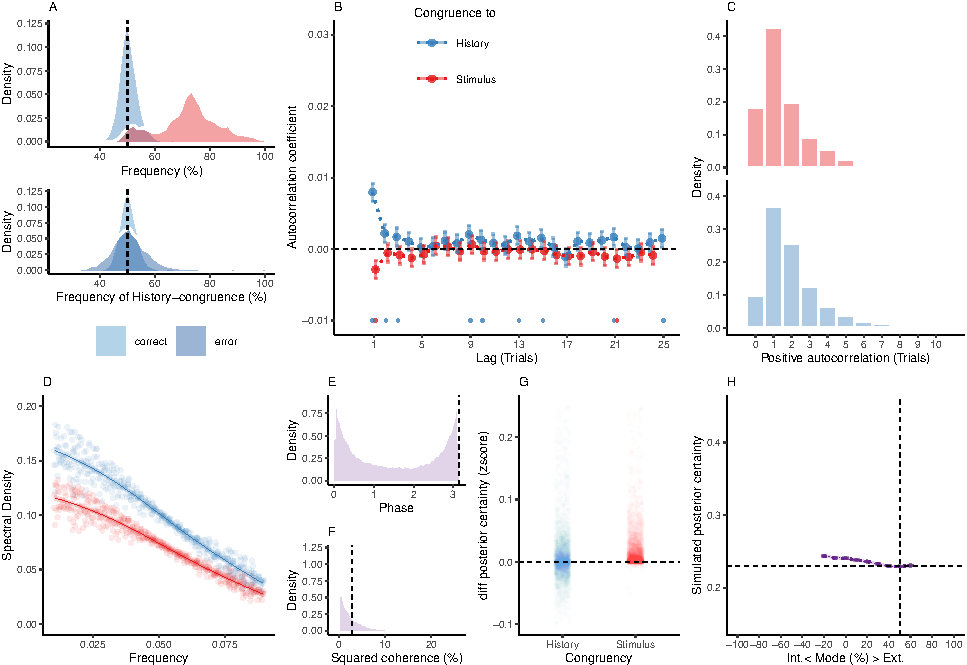
\includegraphics{modes_mouse_files/figure-latex/Supplemental_Figure_S8-1.pdf}

\textbf{Supplemental Figure S8. Reduced Control Model 2: No
oscillations.} When simulating data for the \emph{no-oscillation model},
we removed the oscillation from the likelihood and prior terms by
setting the amplitudes \(a_{LLR}\) and \(a_{\psi}\) to zero. Simulated
data thus depended only on the participant-wise estimates for hazard
rate \(H\) and inverse decision temperature \(\zeta\).

A. Similar to the full model (Figure 6), simulated perceptual choices
were stimulus-congruent in 71.97\% ± 0.17\% of trials (in red).
History-congruent amounted to 50.73\% ± 0.07\% of trials (in blue). As
in the full model, the no-oscillation model showed a significant bias
toward perceptual history T(\ensuremath{4.32\times 10^{3}}) = 9.94, p =
\(\ensuremath{4.88\times 10^{-23}}\); upper panel). Similarly,
history-congruent choices were more frequent at error trials
(T(\ensuremath{4.31\times 10^{3}}) = 10.59, p =
\(\ensuremath{7.02\times 10^{-26}}\); lower panel).

B. In the no-oscillation model, we did not find significant
autocorrelations for stimulus-congruence. Likewise, we did not observe
any autocorrelation of history-congruence beyond the first three
consecutive trials.

C. In the no-oscillation model, the number of consecutive trials at
which true autocorrelation coefficients exceeded the autocorrelation
coefficients for randomly permuted data decreased with respect to both
stimulus-congruence (1.8 ± \ensuremath{1.59\times 10^{-3}} trials;
T(\ensuremath{4.31\times 10^{3}}) = -5.21, p =
\(\ensuremath{2\times 10^{-7}}\)) and history-congruence (2.18 ±
\ensuremath{5.48\times 10^{-4}} trials;
T(\ensuremath{4.32\times 10^{3}}) = -17.1, p =
\(\ensuremath{1.75\times 10^{-63}}\)) relative to the full model.

D. In the no-oscillation model, the smoothed probabilities of stimulus-
and history-congruence (sliding windows of ±5 trials) fluctuated as
\emph{1/f noise}, i.e., at power densities that were inversely
proportional to the frequency (power \textasciitilde{} 1/\(f^\beta\);
stimulus-congruence: \(\beta\) = \(-0.78\) ±
\(\ensuremath{1.1\times 10^{-3}}\),
T(\(\ensuremath{1.92\times 10^{5}}\)) = \(-706.93\), p < \(\ensuremath{2.2\times 10^{-308}}\);
history-congruence: \(\beta\) = \(-0.79\) ±
\(\ensuremath{1.12\times 10^{-3}}\),
T(\(\ensuremath{1.92\times 10^{5}}\)) = \(-702.46\), p < \(\ensuremath{2.2\times 10^{-308}}\)).

E. In the no-oscillation model, the distribution of phase shift between
fluctuations in simulated stimulus- and history-congruence peaked at
half a cycle (\(\pi\) denoted by dotted line). In contrast to the full
model, the dynamic probabilities of simulated stimulus- and
history-congruence were positively correlated (\(\beta\) =
\(\ensuremath{4.3\times 10^{-3}}\) ±
\(\ensuremath{7.97\times 10^{-4}}\),
T(\(\ensuremath{1.98\times 10^{6}}\)) = \(5.4\), p =
\(\ensuremath{6.59\times 10^{-8}}\)).

F. In the no-oscillation model, the average squared coherence between
fluctuations in simulated stimulus- and history-congruence (black dottet
line) was reduced in comparison to the full model
(T(\ensuremath{3.52\times 10^{3}}) = -6.27, p =
\(\ensuremath{3.97\times 10^{-10}}\)) and amounted to 3.26 ±
\ensuremath{8.88\times 10^{-4}}\%.

G. Similar to the full model, confidence simulated from the
no-oscillation model was enhanced for stimulus-congruent choices
(\(\beta\) = \(0.01\) ± \(\ensuremath{1.05\times 10^{-4}}\),
T(\(\ensuremath{2.1\times 10^{6}}\)) = \(139.17\), p < \(\ensuremath{2.2\times 10^{-308}}\)) and
history-congruent choices (\(\beta\) =
\(\ensuremath{8.05\times 10^{-3}}\) ±
\(\ensuremath{9.2\times 10^{-5}}\), T(\(\ensuremath{2.1\times 10^{6}}\))
= \(87.54\), p < \(\ensuremath{2.2\times 10^{-308}}\)).

H. In the no-oscillation model, the positive quadratic relationship
between the mode of perceptual processing and confidence was markedly
reduced in comparison to the full model (\(\beta_2\) = \(0.14\) ±
\(0.07\), T(\(\ensuremath{2.1\times 10^{6}}\)) = \(1.95\), p =
\(0.05\)). The horizontal and vertical dotted lines indicate minimum
posterior certainty and the associated mode, respectively.

\newpage

\hypertarget{supplemental-figure-s9}{%
\subsection{Supplemental Figure S9}\label{supplemental-figure-s9}}

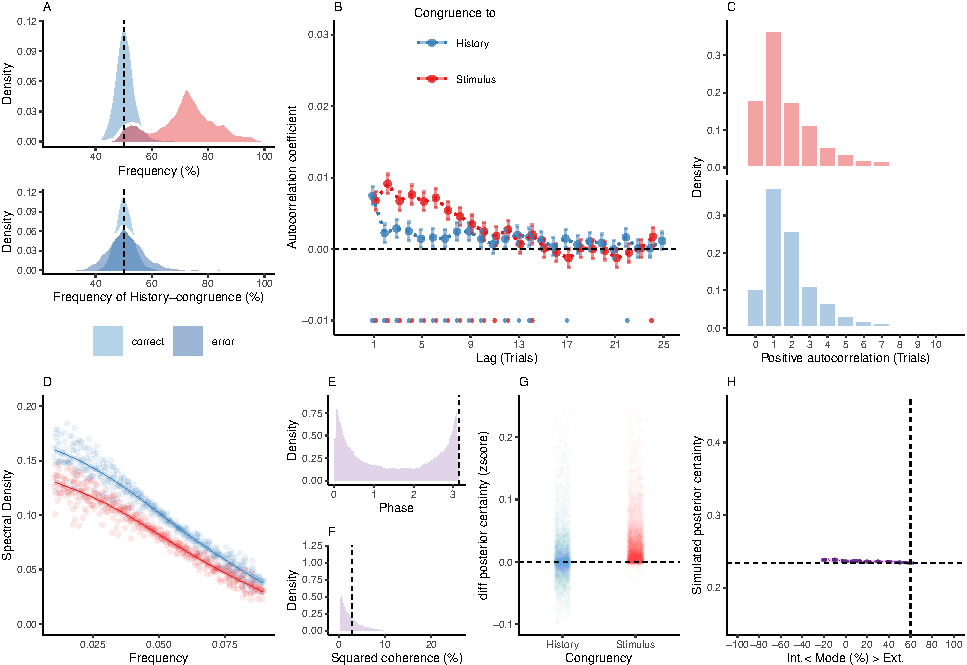
\includegraphics{modes_mouse_files/figure-latex/Supplemental_Figure_S9-1.pdf}

\textbf{Supplemental Figure S9. Reduced Control Model 3: Only
oscillation of the likelihood.} When simulating data for the
\emph{likelihood-oscillation-only model}, we removed the oscillation
from the prior term by setting the amplitude \(a_{\psi}\) to zero.
Simulated data thus depended only on the participant-wise estimates for
hazard rate \(H\), amplitude \(a_{LLR}\), frequency \(f\), phase \(p\)
and inverse decision temperature \(\zeta\).

A. Similar to the full model (Figure 6), simulated perceptual choices
were stimulus-congruent in 71.97\% ± 0.17\% of trials (in red).
History-congruent amounted to 50.76\% ± 0.07\% of trials (in blue). As
in the full model, the likelihood-oscillation-only model showed a
significant bias toward perceptual history
T(\ensuremath{4.32\times 10^{3}}) = 10.29, p =
\(\ensuremath{1.54\times 10^{-24}}\); upper panel). Similarly,
history-congruent choices were more frequent at error trials
(T(\ensuremath{4.32\times 10^{3}}) = 9.71, p =
\(\ensuremath{4.6\times 10^{-22}}\); lower panel).

B. In the likelihood-oscillation-only model, we observed that the
autocorrelation coefficients for history-congruence were reduced below
the autocorrelation coefficients of stimulus-congruence. This is an
approximately five-fold reduction relative to the empirical results
observed in humans (Figure 2B), where the autocorrelation of
history-congruence was above the autocorrelation of stimulus-congruence.
Moreover, in the reduced model shown here, the number of consecutive
trials that showed significant autocorrelation of history-congruence was
reduced to 11.

C. In the likelihood-oscillation-only model, the number of consecutive
trials at which true autocorrelation coefficients exceeded the
autocorrelation coefficients for randomly permuted data did not differ
with respect to stimulus-congruence (2.62 ±
\ensuremath{1.39\times 10^{-3}} trials;
T(\ensuremath{4.32\times 10^{3}}) = 1.85, p = \(0.06\)), but decreased
with respect to history-congruence (2.4 ±
\ensuremath{8.45\times 10^{-4}} trials;
T(\ensuremath{4.32\times 10^{3}}) = -15.26, p =
\(\ensuremath{3.11\times 10^{-51}}\)) relative to the full model.

D. In the likelihood-oscillation-only model, the smoothed probabilities
of stimulus- and history-congruence (sliding windows of ±5 trials)
fluctuated as \emph{1/f noise}, i.e., at power densities that were
inversely proportional to the frequency (power \textasciitilde{}
1/\(f^\beta\); stimulus-congruence: \(\beta\) = \(-0.81\) ±
\(\ensuremath{1.17\times 10^{-3}}\),
T(\(\ensuremath{1.92\times 10^{5}}\)) = \(-688.65\), p < \(\ensuremath{2.2\times 10^{-308}}\);
history-congruence: \(\beta\) = \(-0.79\) ±
\(\ensuremath{1.14\times 10^{-3}}\),
T(\(\ensuremath{1.92\times 10^{5}}\)) = \(-698.13\), p < \(\ensuremath{2.2\times 10^{-308}}\)).

E. In the likelihood-oscillation-only model, the distribution of phase
shift between fluctuations in simulated stimulus- and history-congruence
peaked at half a cycle (\(\pi\) denoted by dotted line). In contrast to
the full model, the dynamic probabilities of simulated stimulus- and
history-congruence were positively correlated (\(\beta\) =
\(\ensuremath{2.7\times 10^{-3}}\) ± \(\ensuremath{7.6\times 10^{-4}}\),
T(\(\ensuremath{2.02\times 10^{6}}\)) = \(3.55\), p =
\(\ensuremath{3.8\times 10^{-4}}\)).

F. In the likelihood-oscillation-only model, the average squared
coherence between fluctuations in simulated stimulus- and
history-congruence (black dottet line) was reduced in comparison to the
full model (T(\ensuremath{3.51\times 10^{3}}) = -4.56, p =
\(\ensuremath{5.27\times 10^{-6}}\)) and amounted to 3.43 ±
\ensuremath{1.02\times 10^{-3}}\%.

G. Similar to the full model, confidence simulated from the
likelihood-oscillation-only model was enhanced for stimulus-congruent
choices (\(\beta\) = \(0.03\) ± \(\ensuremath{1.42\times 10^{-4}}\),
T(\(\ensuremath{2.1\times 10^{6}}\)) = \(191.78\), p < \(\ensuremath{2.2\times 10^{-308}}\)) and
history-congruent choices (\(\beta\) =
\(\ensuremath{9.1\times 10^{-3}}\) ±
\(\ensuremath{1.25\times 10^{-4}}\),
T(\(\ensuremath{2.1\times 10^{6}}\)) = \(72.51\), p < \(\ensuremath{2.2\times 10^{-308}}\)).

H. In the likelihood-oscillation-only model, the positive quadratic
relationship between the mode of perceptual processing and confidence
was markedly reduced in comparison to the full model (\(\beta_2\) =
\(0.34\) ± \(0.1\), T(\(\ensuremath{2.1\times 10^{6}}\)) = \(3.49\), p =
\(\ensuremath{4.78\times 10^{-4}}\)). The horizontal and vertical dotted
lines indicate minimum posterior certainty and the associated mode,
respectively.

\newpage

\hypertarget{supplemental-figure-s10}{%
\subsection{Supplemental Figure S10}\label{supplemental-figure-s10}}

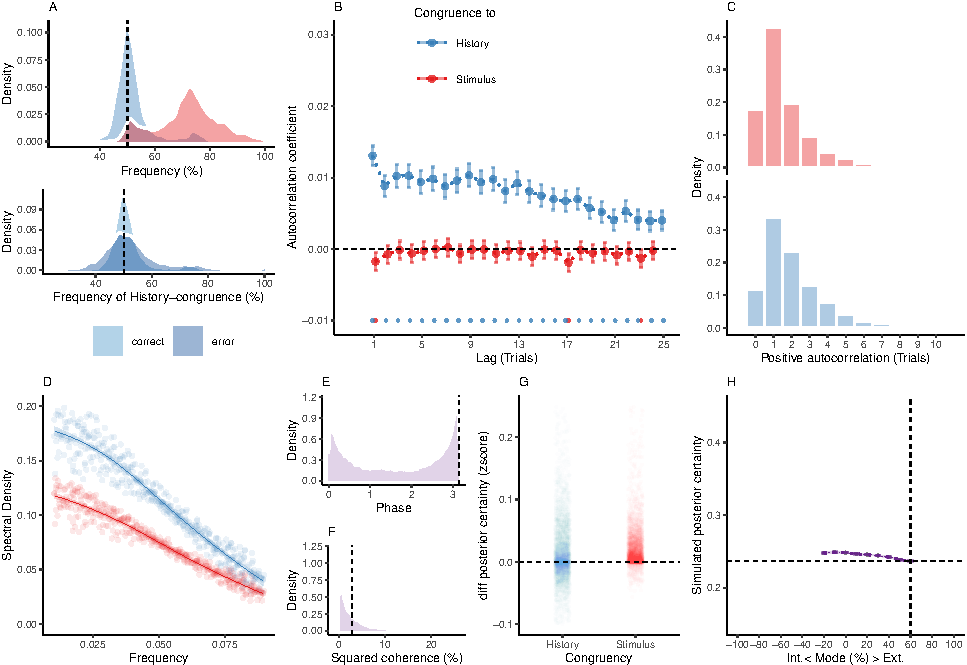
\includegraphics{modes_mouse_files/figure-latex/Supplemental_Figure_S10-1.pdf}

\textbf{Supplemental Figure S10. Reduced Control Model 4: Only
oscillation of the prior.} When simulating data for the
\emph{prior-oscillation-only model}, we removed the oscillation from the
prior term by setting the amplitude \(a_{LLR}\) to zero. Simulated data
thus depended only on the participant-wise estimates for hazard rate
\(H\), amplitude \(a_{\psi}\), frequency \(f\), phase \(p\) and inverse
decision temperature \(\zeta\).

A. Similar to the full model (Figure 6), simulated perceptual choices
were stimulus-congruent in 71.97\% ± 0.17\% of trials (in red).
History-congruent amounted to 52.1\% ± 0.11\% of trials (in blue). As in
the full model, the prior-oscillation-only showed a significant bias
toward perceptual history T(\ensuremath{4.32\times 10^{3}}) = 18.34, p =
\(\ensuremath{1.98\times 10^{-72}}\); upper panel). Similarly,
history-congruent choices were more frequent at error trials
(T(\ensuremath{4.31\times 10^{3}}) = 12.35, p =
\(\ensuremath{1.88\times 10^{-34}}\); lower panel).

B. In the prior-oscillation-only model, we did not observe any
significant positive autocorrelation of stimulus-congruence , whereas
the autocorrelation of history-congruence was preserved.

C. In the prior-oscillation-only model, the number of consecutive trials
at which true autocorrelation coefficients exceeded the autocorrelation
coefficients for randomly permuted data did was decreased with respect
to stimulus-congruence relative to the full model (1.8 ±
\ensuremath{1.01\times 10^{-3}} trials;
T(\ensuremath{4.31\times 10^{3}}) = -6.48, p =
\(\ensuremath{1.03\times 10^{-10}}\)), but did not differ from the full
model with respect to history-congruence (4.25 ±
\ensuremath{1.84\times 10^{-3}} trials;
T(\ensuremath{4.32\times 10^{3}}) = 0.07, p = \(0.95\)).

D. In the prior-oscillation-only model, the smoothed probabilities of
stimulus- and history-congruence (sliding windows of ±5 trials)
fluctuated as \emph{1/f noise}, i.e., at power densities that were
inversely proportional to the frequency (power \textasciitilde{}
1/\(f^\beta\); stimulus-congruence: \(\beta\) = \(-0.78\) ±
\(\ensuremath{1.11\times 10^{-3}}\),
T(\(\ensuremath{1.92\times 10^{5}}\)) = \(-706.62\), p < \(\ensuremath{2.2\times 10^{-308}}\);
history-congruence: \(\beta\) = \(-0.83\) ±
\(\ensuremath{1.27\times 10^{-3}}\),
T(\(\ensuremath{1.92\times 10^{5}}\)) = \(-651.6\), p < \(\ensuremath{2.2\times 10^{-308}}\)).

E. In the prior-oscillation-only model, the distribution of phase shift
between fluctuations in simulated stimulus- and history-congruence
peaked at half a cycle (\(\pi\) denoted by dotted line). Similar to the
full model, the dynamic probabilities of simulated stimulus- and
history-congruence were anti-correlated (\(\beta\) = \(-0.03\) ±
\(\ensuremath{8.61\times 10^{-4}}\),
T(\(\ensuremath{2.12\times 10^{6}}\)) = \(-34.03\), p =
\(\ensuremath{8.17\times 10^{-254}}\)).

F. In the prior-oscillation-only model, the average squared coherence
between fluctuations in simulated stimulus- and history-congruence
(black dottet line) was reduced in comparison to the full model
(T(\ensuremath{3.54\times 10^{3}}) = -3.22, p =
\(\ensuremath{1.28\times 10^{-3}}\)) and amounted to 3.52 ±
\ensuremath{1.04\times 10^{-3}}\%.

G. Similar to the full model, confidence simulated from the
prior-oscillation-only model was enhanced for stimulus-congruent choices
(\(\beta\) = \(0.02\) ± \(\ensuremath{1.44\times 10^{-4}}\),
T(\(\ensuremath{2.03\times 10^{6}}\)) = \(128.53\), p < \(\ensuremath{2.2\times 10^{-308}}\)) and
history-congruent choices (\(\beta\) = \(0.01\) ±
\(\ensuremath{1.26\times 10^{-4}}\),
T(\(\ensuremath{2.03\times 10^{6}}\)) = \(88.24\), p < \(\ensuremath{2.2\times 10^{-308}}\)).

H. In contrast to the full model, the prior-oscillation-only model did
not yield a positive quadratic relationship between the mode of
perceptual processing and confidence (\(\beta_2\) = \(-0.17\) ± \(0.1\),
T(\(\ensuremath{2.04\times 10^{6}}\)) = \(-1.66\), p = \(0.1\)). The
horizontal and vertical dotted lines indicate minimum posterior
certainty and the associated mode, respectively.

\newpage

\hypertarget{supplemental-table-t1}{%
\subsection{Supplemental Table T1}\label{supplemental-table-t1}}

\begingroup\fontsize{7}{9}\selectfont

\begin{longtable}[t]{llr}
\toprule
Authors & Journal & Year\\
\midrule
\endfirsthead
\multicolumn{3}{@{}l}{\textit{(continued)}}\\
\toprule
Authors & Journal & Year\\
\midrule
\endhead

\endfoot
\bottomrule
\endlastfoot
Bang, Shekhar, Rahnev & JEP:General & 2019\\
Bang, Shekhar, Rahnev & JEP:General & 2019\\
Calder-Travis, Charles,  Bogacz, Yeung & Unpublished & NA\\
Clark \& Merfeld & Journal of Neurophysiology & 2018\\
Clark & Unpublished & NA\\
\addlinespace
Faivre, Filevich, Solovey, Kuhn, Blanke & Journal of Neuroscience & 2018\\
Faivre, Vuillaume, Blanke, Cleeremans & bioRxiv & 2018\\
Filevich \& Fandakova & Unplublished & NA\\
Gajdos, Fleming, Saez Garcia, Weindel, Davranche & Neuroscience of Consciousness & 2019\\
Gherman \& Philiastides & eLife & 2018\\
\addlinespace
Haddara \& Rahnev & PsyArXiv & 2020\\
Haddara \& Rahnev & PsyArXiv & 2020\\
Hainguerlot, Vergnaud, \& de Gardelle & Scientific Reports & 2018\\
Hainguerlot, Gajdos, Vergnaud, \& de Gardelle & Unpublished & NA\\
Jachs, Blanco, Grantham-Hill, Soto & JEP:HPP & 2015\\
\addlinespace
Jachs, Blanco, Grantham-Hill, Soto & JEP:HPP & 2015\\
Jachs, Blanco, Grantham-Hill, Soto & JEP:HPP & 2015\\
Jaquiery, Yeung & Unpublished & NA\\
Kvam, Pleskac, Yu, Busemeyer & PNAS & 2015\\
Kvam, Pleskac, Yu, Busemeyer & PNAS & 2015\\
\addlinespace
Kvam and Pleskac & Cognition & 2016\\
Law, Lee & Unpublished & NA\\
Lebreton, et al. & Sci. Advances & 2018\\
Lempert, Chen, \& Fleming & PlosOne & 2015\\
Locke*, Gaffin-Cahn*, Hosseinizaveh, Mamassian, \& Landy & Attention, Perception, \& Psychophysics & 2020\\
\addlinespace
Maniscalco, McCurdy,Odegaard, \& Lau & J Neurosci & 2017\\
Maniscalco, McCurdy,Odegaard, \& Lau & J Neurosci & 2017\\
Maniscalco, McCurdy,Odegaard, \& Lau & J Neurosci & 2017\\
Maniscalco, McCurdy,Odegaard, \& Lau & J Neurosci & 2017\\
Martin, Hsu & Unpublished & NA\\
\addlinespace
Massoni \& Roux & Journal of Mathematical Psychology & 2017\\
Massoni & Unpublished & NA\\
Mazor, Friston \& Fleming & eLife & 2020\\
Mei, Rankine,Olafsson, Soto & bioRxiv & 2019\\
Mei, Rankine,Olafsson, Soto & bioRxiv & 2019\\
\addlinespace
O'Hora, Zgonnikov, Kenny, Wong-Lin & Fechner Day proceedings & 2017\\
O'Hora, Zgonnikov, CiChocki & Unpublished & NA\\
O'Hora, Zgonnikov, Neverauskaite & Unpublished & NA\\
Palser et al & Consciousness \& Cognition & 2018\\
Pereira, Faivre, Iturrate et al. & bioRxiv & 2018\\
\addlinespace
Prieto et al. & Submitted & NA\\
Rahnev et al & J Neurophysiol & 2013\\
Rausch \& Zehetleitner & Front Psychol & 2016\\
Rausch et al & Attention, Perception, \& Psychophysics & 2018\\
Rausch et al & Attention, Perception, \& Psychophysics & 2018\\
\addlinespace
Rausch, Zehetleitner, Steinhauser, \& Maier & NeuroImage & 2020\\
Recht, de Gardelle \& Mamassian & Unpublished & NA\\
Reyes et al. & PlosOne & 2015\\
Reyes et al. & Submitted & NA\\
Rouault, Seow, Gillan, Fleming & Biol. Psychiatry & 2018\\
\addlinespace
Rouault, Seow, Gillan, Fleming & Biol. Psychiatry & 2018\\
Rouault, Dayan, Fleming & Nat Commun & 2019\\
Sadeghi et al & Scientific Reports & 2017\\
Schmidt et al. & Consc Cog & 2019\\
Shekhar \& Rahnev & J Neuroscience & 2018\\
\addlinespace
Shekhar \& Rahnev & PsyArXiv & 2020\\
Sherman et al & Journal of Neuroscience & 2016\\
Sherman et al & Journal of Cognitive Neuroscience & 2016\\
Sherman et al & Unpublished & NA\\
Sherman et al & Unpublished & NA\\
\addlinespace
Siedlecka, Wereszczywski, Paulewicz, Wierzchon & bioRxiv & 2019\\
Song et al & Consciousness \& Cognition & 2011\\
van Boxtel, Orchard, Tsuchiya & bioRxiv & 2019\\
van Boxtel, Orchard, Tsuchiya & bioRxiv & 2019\\
Wierzchon, Paulewicz, Asanowicz, Timmermans \& Cleeremans & Consciousness and Cognition & 2014\\
\addlinespace
Wierzchon, Anzulewicz, Hobot, Paulewicz \& Sackur & Consciousness and Cognition & 2019\\*
\end{longtable}
\endgroup{}

\newpage

\hypertarget{references}{%
\section*{References}\label{references}}
\addcontentsline{toc}{section}{References}

\hypertarget{refs}{}
\begin{CSLReferences}{0}{0}
\leavevmode\vadjust pre{\hypertarget{ref-Schrodinger1944}{}}%
\CSLLeftMargin{1. }%
\CSLRightInline{Schrödinger, E.
\emph{\href{http://filf.pskgu.ru/ebooks/schbio/schbio_titul.pdf}{{What
is Life? The Physical Aspect of the Living Cell}}}. (Cambridge
University Press, 1944).}

\leavevmode\vadjust pre{\hypertarget{ref-Ashby1947}{}}%
\CSLLeftMargin{2. }%
\CSLRightInline{Ashby, W. R.
\href{https://doi.org/10.1080/00221309.1947.9918144}{{Principles of the
self-organizing dynamic system}}. \emph{Journal of General Psychology}
\textbf{37}, 125--128 (1947).}

\leavevmode\vadjust pre{\hypertarget{ref-Friston2013}{}}%
\CSLLeftMargin{3. }%
\CSLRightInline{Friston, K.
\href{https://doi.org/10.1098/rsif.2013.0475}{{Life as we know it}}.
\emph{Journal of The Royal Society Interface} \textbf{10}, 20130475
(2013).}

\leavevmode\vadjust pre{\hypertarget{ref-Palva2011}{}}%
\CSLLeftMargin{4. }%
\CSLRightInline{Palva, J. M. \emph{et al.}
\href{https://doi.org/10.1016/B978-0-444-53839-0.00022-3}{{Roles of
multiscale brain activity fluctuations in shaping the variability and
dynamics of psychophysical performance}}. in \emph{Progress in brain
research} vol. 193 335--350 (Elsevier B.V., 2011).}

\leavevmode\vadjust pre{\hypertarget{ref-VanRullen2016}{}}%
\CSLLeftMargin{5. }%
\CSLRightInline{VanRullen, R.
\href{https://doi.org/10.1016/j.tics.2016.07.006}{{Perceptual Cycles}}.
\emph{Trends in Cognitive Sciences} \textbf{20}, 723--735 (2016).}

\leavevmode\vadjust pre{\hypertarget{ref-Verplanck1952}{}}%
\CSLLeftMargin{6. }%
\CSLRightInline{Verplanck, W. S. \emph{et al.}
\href{https://doi.org/10.1037/h0054948}{{Nonindependence of successive
responses in measurements of the visual threshold}}. \emph{Journal of
Experimental Psychology} \textbf{44}, 273--282 (1952).}

\leavevmode\vadjust pre{\hypertarget{ref-Atkinson1963}{}}%
\CSLLeftMargin{7. }%
\CSLRightInline{Atkinson, R. C.
\href{https://doi.org/10.1037/h0041428}{{A variable sensitivity theory
of signal detection}}. \emph{Psychological Review} \textbf{70}, 91--106
(1963).}

\leavevmode\vadjust pre{\hypertarget{ref-Dehaene1993}{}}%
\CSLLeftMargin{8. }%
\CSLRightInline{Dehaene, S.
\href{https://doi.org/10.1111/j.1467-9280.1993.tb00273.x}{{Temporal
Oscillations in Human Perception}}. \emph{Psychological Science}
\textbf{4}, 264--270 (1993).}

\leavevmode\vadjust pre{\hypertarget{ref-Gilden1995}{}}%
\CSLLeftMargin{9. }%
\CSLRightInline{Gilden, D. L. \emph{et al.}
\href{https://doi.org/10.1006/cogp.1995.1002}{{On the Nature of Streaks
in Signal Detection}}. \emph{Cognitive Psychology} \textbf{28}, 17--64
(1995).}

\leavevmode\vadjust pre{\hypertarget{ref-Gilden1995a}{}}%
\CSLLeftMargin{10. }%
\CSLRightInline{Gilden, D. L. \emph{et al.}
\href{https://doi.org/10.1126/science.7892611}{1/f noise in human
cognition}. \emph{Science} \textbf{67}, 1837--1839 (1995).}

\leavevmode\vadjust pre{\hypertarget{ref-Monto2008}{}}%
\CSLLeftMargin{11. }%
\CSLRightInline{Monto, S. \emph{et al.}
\href{https://doi.org/10.1523/JNEUROSCI.1910-08.2008}{{Very slow EEG
fluctuations predict the dynamics of stimulus detection and oscillation
amplitudes in humans}}. \emph{Journal of Neuroscience} \textbf{28},
8268--8272 (2008).}

\leavevmode\vadjust pre{\hypertarget{ref-Ashwood2022}{}}%
\CSLLeftMargin{12. }%
\CSLRightInline{Ashwood, Z. C. \emph{et al.}
\href{https://doi.org/10.1038/s41593-021-01007-z}{{Mice alternate
between discrete strategies during perceptual decision-making}}.
\emph{Nature Neuroscience} \textbf{25}, 201--212 (2022).}

\leavevmode\vadjust pre{\hypertarget{ref-Gilden2001}{}}%
\CSLLeftMargin{13. }%
\CSLRightInline{Gilden, D. L.
\href{https://doi.org/10.1037/0033-295X.108.1.33}{{Cognitive emissions
of 1/f noise}}. \emph{Psychological Review} \textbf{108}, 33--56
(2001).}

\leavevmode\vadjust pre{\hypertarget{ref-Duncan2012}{}}%
\CSLLeftMargin{14. }%
\CSLRightInline{Duncan, K. \emph{et al.}
\href{https://doi.org/10.1126/science.1221936}{{Memory's Penumbra:
Episodic memory decisions induce lingering mnemonic biases}}.
\emph{Science} \textbf{337}, 485--487 (2012).}

\leavevmode\vadjust pre{\hypertarget{ref-ClareKelly2008}{}}%
\CSLLeftMargin{15. }%
\CSLRightInline{Clare Kelly, A. M. \emph{et al.}
\href{https://doi.org/10.1016/j.neuroimage.2007.08.008}{{Competition
between functional brain networks mediates behavioral variability}}.
\emph{NeuroImage} \textbf{39}, 527--537 (2008).}

\leavevmode\vadjust pre{\hypertarget{ref-Hesselmann2008}{}}%
\CSLLeftMargin{16. }%
\CSLRightInline{Hesselmann, G. \emph{et al.}
\href{https://doi.org/10.1073/pnas.0712043105}{{Spontaneous local
variations in ongoing neural activity bias perceptual decisions}}.
\emph{Proceedings of the National Academy of Sciences of the United
States of America} \textbf{105}, 10984--10989 (2008).}

\leavevmode\vadjust pre{\hypertarget{ref-Schroeder2010a}{}}%
\CSLLeftMargin{17. }%
\CSLRightInline{Schroeder, C. E. \emph{et al.}
\href{https://doi.org/10.1016/j.conb.2010.02.010}{{Dynamics of Active
Sensing and perceptual selection}}. \emph{Current Opinion in
Neurobiology} \textbf{20}, 172--176 (2010).}

\leavevmode\vadjust pre{\hypertarget{ref-Honey2017}{}}%
\CSLLeftMargin{18. }%
\CSLRightInline{Honey, C. J. \emph{et al.}
\href{https://doi.org/10.1162/netn_a_00024}{{Switching between internal
and external modes: A multiscale learning principle}}. \emph{Network
Neuroscience} \textbf{1}, 339--356 (2017).}

\leavevmode\vadjust pre{\hypertarget{ref-Weilnhammer2021a}{}}%
\CSLLeftMargin{19. }%
\CSLRightInline{Weilnhammer, V. \emph{et al.}
\href{https://doi.org/10.1016/j.isci.2021.102234}{{Bistable perception
alternates between internal and external modes of sensory processing}}.
\emph{iScience} \textbf{24}, (2021).}

\leavevmode\vadjust pre{\hypertarget{ref-Rahnev2020}{}}%
\CSLLeftMargin{20. }%
\CSLRightInline{Rahnev, D. \emph{et al.}
\href{https://doi.org/10.1038/s41562-019-0813-1}{{The Confidence
Database}}. \emph{Nature Human Behaviour} \textbf{4}, 317--325 (2020).}

\leavevmode\vadjust pre{\hypertarget{ref-Aguillon-Rodriguez2020}{}}%
\CSLLeftMargin{21. }%
\CSLRightInline{The International Brain Laboratory. {Standardized and
reproducible measurement of decision-making in mice}. \emph{bioRxiv}
2020.01.17.909838 (2020)
doi:\href{https://doi.org/10.1101/2020.01.17.909838}{10.1101/2020.01.17.909838}.}

\leavevmode\vadjust pre{\hypertarget{ref-fischer_serial_2014}{}}%
\CSLLeftMargin{22. }%
\CSLRightInline{Fischer, J. \emph{et al.}
\href{https://doi.org/10.1038/nn.3689}{{Serial dependence in visual
perception}}. \emph{Nat. Neurosci.} \textbf{17}, 738--743 (2014).}

\leavevmode\vadjust pre{\hypertarget{ref-Liberman2014}{}}%
\CSLLeftMargin{23. }%
\CSLRightInline{Liberman, A. \emph{et al.}
\href{https://doi.org/10.1016/j.cub.2014.09.025}{{Serial dependence in
the perception of faces}}. \emph{Current Biology} \textbf{24},
2569--2574 (2014).}

\leavevmode\vadjust pre{\hypertarget{ref-Abrahamyan2016}{}}%
\CSLLeftMargin{24. }%
\CSLRightInline{Abrahamyan, A. \emph{et al.}
\href{https://doi.org/10.1073/pnas.1518786113}{{Adaptable history biases
in human perceptual decisions}}. \emph{Proceedings of the National
Academy of Sciences of the United States of America} \textbf{113},
E3548--E3557 (2016).}

\leavevmode\vadjust pre{\hypertarget{ref-Cicchini2014}{}}%
\CSLLeftMargin{25. }%
\CSLRightInline{Cicchini, G. M. \emph{et al.}
\href{https://doi.org/10.1073/pnas.1402785111}{{Compressive mapping of
number to space reflects dynamic encoding mechanisms, not static
logarithmic transform}}. \emph{Proceedings of the National Academy of
Sciences of the United States of America} \textbf{111}, 7867--7872
(2014).}

\leavevmode\vadjust pre{\hypertarget{ref-Cicchini2017}{}}%
\CSLLeftMargin{26. }%
\CSLRightInline{Cicchini, G. M. \emph{et al.}
\href{https://doi.org/10.1167/17.14.6}{{Serial dependencies act directly
on perception}}. \emph{Journal of Vision} \textbf{17}, (2017).}

\leavevmode\vadjust pre{\hypertarget{ref-Fritsche2020}{}}%
\CSLLeftMargin{27. }%
\CSLRightInline{Fritsche, M. \emph{et al.}
\href{https://doi.org/10.7554/eLife.55389}{{A bayesian and efficient
observer model explains concurrent attractive and repulsive history
biases in visual perception}}. \emph{eLife} \textbf{9}, 1--32 (2020).}

\leavevmode\vadjust pre{\hypertarget{ref-Urai2017}{}}%
\CSLLeftMargin{28. }%
\CSLRightInline{Urai, A. E. \emph{et al.}
\href{https://doi.org/10.1038/ncomms14637}{{Pupil-linked arousal is
driven by decision uncertainty and alters serial choice bias}}.
\emph{Nature Communications} \textbf{8}, (2017).}

\leavevmode\vadjust pre{\hypertarget{ref-Akrami2018}{}}%
\CSLLeftMargin{29. }%
\CSLRightInline{Akrami, A. \emph{et al.}
\href{https://doi.org/10.1038/nature25510}{{Posterior parietal cortex
represents sensory history and mediates its effects on behaviour}}.
\emph{Nature} \textbf{554}, 368--372 (2018).}

\leavevmode\vadjust pre{\hypertarget{ref-Braun2018}{}}%
\CSLLeftMargin{30. }%
\CSLRightInline{Braun, A. \emph{et al.}
\href{https://doi.org/10.1523/JNEUROSCI.2189-17.2017}{{Adaptive history
biases result from confidence-weighted accumulation of past choices}}.
\emph{Journal of Neuroscience} \textbf{38}, 2418--2429 (2018).}

\leavevmode\vadjust pre{\hypertarget{ref-Bergen2019}{}}%
\CSLLeftMargin{31. }%
\CSLRightInline{Bergen, R. S. V. \emph{et al.}
\href{https://doi.org/10.1523/JNEUROSCI.3212-18.2019}{{Probabilistic
representation in human visual cortex reflects uncertainty in serial
decisions}}. \emph{Journal of Neuroscience} \textbf{39}, 8164--8176
(2019).}

\leavevmode\vadjust pre{\hypertarget{ref-Urai2019}{}}%
\CSLLeftMargin{32. }%
\CSLRightInline{Urai, A. E. \emph{et al.}
\href{https://doi.org/10.7554/eLife.46331}{{Choice history biases
subsequent evidence accumulation}}. \emph{eLife} \textbf{8}, (2019).}

\leavevmode\vadjust pre{\hypertarget{ref-Hsu2020}{}}%
\CSLLeftMargin{33. }%
\CSLRightInline{Hsu, S. M. \emph{et al.}
\href{https://doi.org/10.1080/02699931.2019.1696752}{{The roles of
preceding stimuli and preceding responses on assimilative and
contrastive sequential effects during facial expression perception}}.
\emph{Cognition and Emotion} \textbf{34}, 890--905 (2020).}

\leavevmode\vadjust pre{\hypertarget{ref-Dong1995}{}}%
\CSLLeftMargin{34. }%
\CSLRightInline{Dong, D. W. \emph{et al.}
\href{https://doi.org/10.1088/0954-898X_6_3_003}{{Statistics of natural
time-varying images}}. \emph{Network: Computation in Neural Systems}
\textbf{6}, 345--358 (1995).}

\leavevmode\vadjust pre{\hypertarget{ref-Burr2014}{}}%
\CSLLeftMargin{35. }%
\CSLRightInline{Burr, D. \emph{et al.}
\href{https://doi.org/10.1016/j.cub.2014.10.002}{{Vision: Efficient
adaptive coding}}. \emph{Current Biology} \textbf{24}, R1096--R1098
(2014).}

\leavevmode\vadjust pre{\hypertarget{ref-Montroll1982}{}}%
\CSLLeftMargin{36. }%
\CSLRightInline{Montroll, E. W. \emph{et al.}
\href{https://doi.org/10.1073/pnas.79.10.3380}{{On 1/f noise and other
distributions with long tails}}. \emph{Proceedings of the National
Academy of Sciences} \textbf{79}, 3380--3383 (1982).}

\leavevmode\vadjust pre{\hypertarget{ref-Bak1987}{}}%
\CSLLeftMargin{37. }%
\CSLRightInline{Bak, P. \emph{et al.}
\href{https://doi.org/10.1103/PhysRevLett.59.381}{{Self-organized
criticality: An explanation of the 1/f noise}}. \emph{Physical Review
Letters} \textbf{59}, 381--384 (1987).}

\leavevmode\vadjust pre{\hypertarget{ref-Chialvo2010}{}}%
\CSLLeftMargin{38. }%
\CSLRightInline{Chialvo, D. R.
\href{https://doi.org/10.1038/nphys1803}{{Emergent complex neural
dynamics}}. \emph{Nature Physics} \textbf{6}, 744--750 (2010).}

\leavevmode\vadjust pre{\hypertarget{ref-Wagenmakers2004}{}}%
\CSLLeftMargin{39. }%
\CSLRightInline{Wagenmakers, E. J. \emph{et al.}
\href{https://doi.org/10.3758/BF03196615}{{Estimation and interpretation
of 1/f\(\alpha\) noise in human cognition}}. \emph{Psychonomic Bulletin
and Review} \textbf{11}, 579--615 (2004).}

\leavevmode\vadjust pre{\hypertarget{ref-VanOrden2005}{}}%
\CSLLeftMargin{40. }%
\CSLRightInline{Van Orden, G. C. \emph{et al.}
\href{https://doi.org/10.1037/0096-3445.134.1.117}{{Human cognition and
1/f scaling}}. \emph{Journal of Experimental Psychology: General}
\textbf{134}, 117--123 (2005).}

\leavevmode\vadjust pre{\hypertarget{ref-Chopin2012}{}}%
\CSLLeftMargin{41. }%
\CSLRightInline{Chopin, A. \emph{et al.}
\href{https://doi.org/10.1016/j.cub.2012.02.021}{{Predictive properties
of visual adaptation}}. \emph{Current Biology} \textbf{22}, 622--626
(2012).}

\leavevmode\vadjust pre{\hypertarget{ref-Cicchini2018}{}}%
\CSLLeftMargin{42. }%
\CSLRightInline{Cicchini, G. M. \emph{et al.}
\href{https://doi.org/10.1098/rspb.2018.1722}{{The functional role of
serial dependence}}. \emph{Proceedings of the Royal Society B:
Biological Sciences} \textbf{285}, (2018).}

\leavevmode\vadjust pre{\hypertarget{ref-Kiyonaga2017}{}}%
\CSLLeftMargin{43. }%
\CSLRightInline{Kiyonaga, A. \emph{et al.}
\href{https://doi.org/10.1016/j.tics.2017.04.011}{{Serial Dependence
across Perception, Attention, and Memory}}. \emph{Trends in Cognitive
Sciences} \textbf{21}, 493--497 (2017).}

\leavevmode\vadjust pre{\hypertarget{ref-McGinley2015b}{}}%
\CSLLeftMargin{44. }%
\CSLRightInline{McGinley, M. J. \emph{et al.}
\href{https://doi.org/10.1016/j.neuron.2015.09.012}{{Waking State: Rapid
Variations Modulate Neural and Behavioral Responses}}. \emph{Neuron}
\textbf{87}, 1143--1161 (2015).}

\leavevmode\vadjust pre{\hypertarget{ref-Rosenberg2013}{}}%
\CSLLeftMargin{45. }%
\CSLRightInline{Rosenberg, M. \emph{et al.}
\href{https://doi.org/10.3758/s13414-012-0413-x}{{Sustaining visual
attention in the face of distraction: A novel gradual-onset continuous
performance task}}. \emph{Attention, Perception, and Psychophysics}
\textbf{75}, 426--439 (2013).}

\leavevmode\vadjust pre{\hypertarget{ref-Zalta2020}{}}%
\CSLLeftMargin{46. }%
\CSLRightInline{Zalta, A. \emph{et al.}
\href{https://doi.org/10.1038/s41467-020-14888-8}{{Natural rhythms of
periodic temporal attention}}. \emph{Nature Communications} \textbf{11},
1--12 (2020).}

\leavevmode\vadjust pre{\hypertarget{ref-Prado2011}{}}%
\CSLLeftMargin{47. }%
\CSLRightInline{Prado, J. \emph{et al.}
\href{https://doi.org/10.1016/j.neuroimage.2010.08.022}{{Variations of
response time in a selective attention task are linked to variations of
functional connectivity in the attentional network}}. \emph{NeuroImage}
\textbf{54}, 541--549 (2011).}

\leavevmode\vadjust pre{\hypertarget{ref-St.John-Saaltink2016}{}}%
\CSLLeftMargin{48. }%
\CSLRightInline{St. John-Saaltink, E. \emph{et al.}
\href{https://doi.org/10.1523/JNEUROSCI.4390-15.2016}{{Serial Dependence
in Perceptual Decisions Is Reflected in Activity Patterns in Primary
Visual Cortex}}. \emph{Journal of Neuroscience} \textbf{36}, 6186--6192
(2016).}

\leavevmode\vadjust pre{\hypertarget{ref-Cicchini2021}{}}%
\CSLLeftMargin{49. }%
\CSLRightInline{Cicchini, G. M. \emph{et al.}
\href{https://doi.org/10.1016/j.cub.2020.12.004}{{Perceptual history
propagates down to early levels of sensory analysis}}. \emph{Current
Biology} \textbf{31}, 1245--1250.e2 (2021).}

\leavevmode\vadjust pre{\hypertarget{ref-Kepecs2008}{}}%
\CSLLeftMargin{50. }%
\CSLRightInline{Kepecs, A. \emph{et al.}
\href{https://doi.org/10.1038/nature07200}{{Neural correlates,
computation and behavioural impact of decision confidence}}.
\emph{Nature} \textbf{455}, 227--231 (2008).}

\leavevmode\vadjust pre{\hypertarget{ref-Fleming2014}{}}%
\CSLLeftMargin{51. }%
\CSLRightInline{Fleming, S. M. \emph{et al.}
\href{https://doi.org/10.3389/fnhum.2014.00443}{{How to measure
metacognition}}. \emph{Frontiers in Human Neuroscience} \textbf{8}, 443
(2014).}

\leavevmode\vadjust pre{\hypertarget{ref-Leys2013}{}}%
\CSLLeftMargin{52. }%
\CSLRightInline{Leys, C. \emph{et al.}
\href{https://doi.org/10.1016/J.JESP.2013.03.013}{{Detecting outliers:
Do not use standard deviation around the mean, use absolute deviation
around the median}}. \emph{Journal of Experimental Social Psychology}
\textbf{49}, 764--766 (2013).}

\leavevmode\vadjust pre{\hypertarget{ref-Maloney2005}{}}%
\CSLLeftMargin{53. }%
\CSLRightInline{Maloney, L. T. \emph{et al.}
\href{https://doi.org/10.1073/pnas.0407157102}{{Past trials influence
perception of ambiguous motion quartets through pattern completion}}.
\emph{Proceedings of the National Academy of Sciences of the United
States of America} \textbf{102}, 3164--3169 (2005).}

\leavevmode\vadjust pre{\hypertarget{ref-Glaze2015}{}}%
\CSLLeftMargin{54. }%
\CSLRightInline{Glaze, C. M. \emph{et al.}
\href{https://doi.org/10.7554/eLife.08825}{{Normative evidence
accumulation in unpredictable environments}}. \emph{eLife} \textbf{4},
(2015).}

\leavevmode\vadjust pre{\hypertarget{ref-Wexler2015}{}}%
\CSLLeftMargin{55. }%
\CSLRightInline{Wexler, M. \emph{et al.}
\href{https://doi.org/10.1073/pnas.1508847112}{{Persistent states in
vision break universality and time invariance}}. \emph{Proceedings of
the National Academy of Sciences of the United States of America}
\textbf{112}, 14990--14995 (2015).}

\leavevmode\vadjust pre{\hypertarget{ref-Rao1999}{}}%
\CSLLeftMargin{56. }%
\CSLRightInline{Rao, R. P. \emph{et al.}
\href{https://doi.org/10.1038/4580}{{Predictive coding in the visual
cortex: a functional interpretation of some extra-classical
receptive-field effects.}} \emph{Nature neuroscience} \textbf{2}, 79--87
(1999).}

\leavevmode\vadjust pre{\hypertarget{ref-Jardri2017}{}}%
\CSLLeftMargin{57. }%
\CSLRightInline{Jardri, R. \emph{et al.}
\href{https://doi.org/10.1038/ncomms14218}{{Experimental evidence for
circular inference in schizophrenia}}. \emph{Nature Communications}
\textbf{8}, 14218 (2017).}

\leavevmode\vadjust pre{\hypertarget{ref-Guggenmos2016}{}}%
\CSLLeftMargin{58. }%
\CSLRightInline{Guggenmos, M. \emph{et al.}
\href{https://doi.org/10.7554/eLife.13388}{{Mesolimbic confidence
signals guide perceptual learning in the absence of external feedback}}.
\emph{eLife} \textbf{5}, (2016).}

\leavevmode\vadjust pre{\hypertarget{ref-Mathys2014a}{}}%
\CSLLeftMargin{59. }%
\CSLRightInline{Mathys, C. D. \emph{et al.}
\href{https://doi.org/10.3389/fnhum.2014.00825}{{Uncertainty in
perception and the Hierarchical Gaussian Filter.}} \emph{Frontiers in
human neuroscience} \textbf{8}, 825 (2014).}

\leavevmode\vadjust pre{\hypertarget{ref-Sterzer2018}{}}%
\CSLLeftMargin{60. }%
\CSLRightInline{Sterzer, P. \emph{et al.}
\href{https://doi.org/10.1016/j.biopsych.2018.05.015}{{The Predictive
Coding Account of Psychosis}}. \emph{Biological Psychiatry} \textbf{84},
634--643 (2018).}

\leavevmode\vadjust pre{\hypertarget{ref-Bengio2015}{}}%
\CSLLeftMargin{61. }%
\CSLRightInline{Bengio, Y. \emph{et al.}
\href{http://arxiv.org/abs/1502.04156}{{Towards Biologically Plausible
Deep Learning}}. \emph{bioRxiv} (2015).}

\leavevmode\vadjust pre{\hypertarget{ref-Dijkstra2021}{}}%
\CSLLeftMargin{62. }%
\CSLRightInline{Dijkstra, N. \emph{et al.} {Perceptual reality
monitoring: Neural mechanisms dissociating imagination from reality}.
\emph{PsyArXiv} (2021)
doi:\href{https://doi.org/10.31234/OSF.IO/ZNGEQ}{10.31234/OSF.IO/ZNGEQ}.}

\leavevmode\vadjust pre{\hypertarget{ref-Andrillon2021}{}}%
\CSLLeftMargin{63. }%
\CSLRightInline{Andrillon, T. \emph{et al.}
\href{https://doi.org/10.1038/s41467-021-23890-7}{{Predicting lapses of
attention with sleep-like slow waves}}. \emph{Nature Communications}
\textbf{12}, 3657 (2021).}

\leavevmode\vadjust pre{\hypertarget{ref-Passingham}{}}%
\CSLLeftMargin{64. }%
\CSLRightInline{Passingham, R. E. \emph{{Understanding the prefrontal
cortex : selective advantage, connectivity, and neural operations}}.
(Oxford University Press).}

\leavevmode\vadjust pre{\hypertarget{ref-Ashwood2021}{}}%
\CSLLeftMargin{65. }%
\CSLRightInline{Ashwood, Z. C. \emph{et al.} {Mice alternate between
discrete strategies during perceptual decision-making}. \emph{bioRxiv}
2020.10.19.346353 (2021)
doi:\href{https://doi.org/10.1101/2020.10.19.346353}{10.1101/2020.10.19.346353}.}

\leavevmode\vadjust pre{\hypertarget{ref-Bak1996}{}}%
\CSLLeftMargin{66. }%
\CSLRightInline{Bak, P. {Complexity and Criticality}. in \emph{How
nature works} 1--32 (Springer New York, 1996).
doi:\href{https://doi.org/10.1007/978-1-4757-5426-1_1}{10.1007/978-1-4757-5426-1\_1}.}

\leavevmode\vadjust pre{\hypertarget{ref-Deneve2016}{}}%
\CSLLeftMargin{67. }%
\CSLRightInline{Denève, S. \emph{et al.}
\href{https://doi.org/10.1038/nn.4243}{{Efficient codes and balanced
networks}}. \emph{Nature Neuroscience} \textbf{19}, 375--382 (2016).}

\leavevmode\vadjust pre{\hypertarget{ref-Beggs2003}{}}%
\CSLLeftMargin{68. }%
\CSLRightInline{Beggs, J. M. \emph{et al.}
\href{https://doi.org/10.1523/jneurosci.23-35-11167.2003}{{Neuronal
Avalanches in Neocortical Circuits}}. \emph{Journal of Neuroscience}
\textbf{23}, 11167--11177 (2003).}

\leavevmode\vadjust pre{\hypertarget{ref-Wang1999}{}}%
\CSLLeftMargin{69. }%
\CSLRightInline{Wang, X. J.
\href{https://doi.org/10.1523/jneurosci.19-21-09587.1999}{{Synaptic
basis of cortical persistent activity: The importance of NMDA receptors
to working memory}}. \emph{Journal of Neuroscience} \textbf{19},
9587--9603 (1999).}

\leavevmode\vadjust pre{\hypertarget{ref-Wang2001}{}}%
\CSLLeftMargin{70. }%
\CSLRightInline{Wang, X. J.
\href{https://doi.org/10.1016/S0166-2236(00)01868-3}{{Synaptic
reverberation underlying mnemonic persistent activity}}. \emph{Trends in
Neurosciences} \textbf{24}, 455--463 (2001).}

\leavevmode\vadjust pre{\hypertarget{ref-Wang2013}{}}%
\CSLLeftMargin{71. }%
\CSLRightInline{Wang, M. \emph{et al.}
\href{https://doi.org/10.1016/j.neuron.2012.12.032}{{NMDA Receptors
Subserve Persistent Neuronal Firing during Working Memory in
Dorsolateral Prefrontal Cortex}}. \emph{Neuron} \textbf{77}, 736--749
(2013).}

\leavevmode\vadjust pre{\hypertarget{ref-Bliss2017}{}}%
\CSLLeftMargin{72. }%
\CSLRightInline{Bliss, D. P. \emph{et al.}
\href{https://doi.org/10.1371/journal.pone.0188927}{{Synaptic
augmentation in a cortical circuit model reproduces serial dependence in
visual working memory}}. \emph{PLOS ONE} \textbf{12}, e0188927 (2017).}

\leavevmode\vadjust pre{\hypertarget{ref-Stein2020}{}}%
\CSLLeftMargin{73. }%
\CSLRightInline{Stein, H. \emph{et al.}
\href{https://doi.org/10.1038/s41467-020-18033-3}{{Reduced serial
dependence suggests deficits in synaptic potentiation in anti-NMDAR
encephalitis and schizophrenia}}. \emph{Nature Communications}
\textbf{11}, 1--11 (2020).}

\leavevmode\vadjust pre{\hypertarget{ref-Durstewitz2000}{}}%
\CSLLeftMargin{74. }%
\CSLRightInline{Durstewitz, D. \emph{et al.}
\href{https://doi.org/10.1038/81460}{{Neurocomputational Models of
Working Memory}}. \emph{Nature Neuroscience} \textbf{3}, 1184--1191
(2000).}

\leavevmode\vadjust pre{\hypertarget{ref-Seamans2001}{}}%
\CSLLeftMargin{75. }%
\CSLRightInline{Seamans, J. K. \emph{et al.}
\href{https://doi.org/10.1073/pnas.98.1.301}{{Dopamine D1/D5 receptor
modulation of excitatory synaptic inputs to layer V prefrontal cortex
neurons}}. \emph{Proceedings of the National Academy of Sciences of the
United States of America} \textbf{98}, 301--306 (2001).}

\leavevmode\vadjust pre{\hypertarget{ref-Kobayashi2017}{}}%
\CSLLeftMargin{76. }%
\CSLRightInline{Kobayashi, T. \emph{et al.}
\href{https://doi.org/10.1038/s41598-017-02366-z}{{Reproducing
Infra-Slow Oscillations with Dopaminergic Modulation}}. \emph{Scientific
Reports} \textbf{7}, 1--9 (2017).}

\leavevmode\vadjust pre{\hypertarget{ref-Chew2019}{}}%
\CSLLeftMargin{77. }%
\CSLRightInline{Chew, B. \emph{et al.}
\href{https://doi.org/10.1073/pnas.1900872116}{{Endogenous fluctuations
in the dopaminergic midbrain drive behavioral choice variability}}.
\emph{Proceedings of the National Academy of Sciences of the United
States of America} \textbf{116}, 18732--18737 (2019).}

\leavevmode\vadjust pre{\hypertarget{ref-Fritsche2017}{}}%
\CSLLeftMargin{78. }%
\CSLRightInline{Fritsche, M. \emph{et al.}
\href{https://doi.org/10.1016/j.cub.2017.01.006}{{Opposite Effects of
Recent History on Perception and Decision}}. \emph{Current Biology}
\textbf{27}, 590--595 (2017).}

\leavevmode\vadjust pre{\hypertarget{ref-Gekas2019}{}}%
\CSLLeftMargin{79. }%
\CSLRightInline{Gekas, N. \emph{et al.}
\href{https://doi.org/10.1167/19.6.24}{{Disambiguating serial effects of
multiple timescales}}. \emph{Journal of Vision} \textbf{19}, 1--14
(2019).}

\leavevmode\vadjust pre{\hypertarget{ref-Weilnhammer2020}{}}%
\CSLLeftMargin{80. }%
\CSLRightInline{Weilnhammer, V. \emph{et al.}
\href{https://www.ncbi.nlm.nih.gov/pubmed/32090246}{{Psychotic
Experiences in Schizophrenia and Sensitivity to Sensory Evidence.}}
\emph{Schizophrenia bulletin} \textbf{46}, 927--936 (2020).}

\leavevmode\vadjust pre{\hypertarget{ref-Fletcher2009}{}}%
\CSLLeftMargin{81. }%
\CSLRightInline{Fletcher, P. C. \emph{et al.}
\href{https://doi.org/10.1038/nrn2536}{{Perceiving is believing: a
Bayesian approach to explaining the positive symptoms of
schizophrenia.}} \emph{Nature reviews. Neuroscience} \textbf{10}, 48--58
(2009).}

\leavevmode\vadjust pre{\hypertarget{ref-Corlett2019a}{}}%
\CSLLeftMargin{82. }%
\CSLRightInline{Corlett, P. R. \emph{et al.}
\href{https://doi.org/10.1016/j.tics.2018.12.001}{{Hallucinations and
Strong Priors.}} \emph{Tics} \textbf{23}, 114--127 (2019).}

\end{CSLReferences}

\end{document}
